\documentclass[twoside]{book}

% Packages required by doxygen
\usepackage{fixltx2e}
\usepackage{calc}
\usepackage{doxygen}
\usepackage[export]{adjustbox} % also loads graphicx
\usepackage{graphicx}
\usepackage[utf8]{inputenc}
\usepackage{makeidx}
\usepackage{multicol}
\usepackage{multirow}
\PassOptionsToPackage{warn}{textcomp}
\usepackage{textcomp}
\usepackage[nointegrals]{wasysym}
\usepackage[table]{xcolor}

% Font selection
\usepackage[T1]{fontenc}
\usepackage[scaled=.90]{helvet}
\usepackage{courier}
\usepackage{amssymb}
\usepackage{sectsty}
\renewcommand{\familydefault}{\sfdefault}
\allsectionsfont{%
  \fontseries{bc}\selectfont%
  \color{darkgray}%
}
\renewcommand{\DoxyLabelFont}{%
  \fontseries{bc}\selectfont%
  \color{darkgray}%
}
\newcommand{\+}{\discretionary{\mbox{\scriptsize$\hookleftarrow$}}{}{}}

% Page & text layout
\usepackage{geometry}
\geometry{%
  a4paper,%
  top=2.5cm,%
  bottom=2.5cm,%
  left=2.5cm,%
  right=2.5cm%
}
\tolerance=750
\hfuzz=15pt
\hbadness=750
\setlength{\emergencystretch}{15pt}
\setlength{\parindent}{0cm}
\setlength{\parskip}{3ex plus 2ex minus 2ex}
\makeatletter
\renewcommand{\paragraph}{%
  \@startsection{paragraph}{4}{0ex}{-1.0ex}{1.0ex}{%
    \normalfont\normalsize\bfseries\SS@parafont%
  }%
}
\renewcommand{\subparagraph}{%
  \@startsection{subparagraph}{5}{0ex}{-1.0ex}{1.0ex}{%
    \normalfont\normalsize\bfseries\SS@subparafont%
  }%
}
\makeatother

% Headers & footers
\usepackage{fancyhdr}
\pagestyle{fancyplain}
\fancyhead[LE]{\fancyplain{}{\bfseries\thepage}}
\fancyhead[CE]{\fancyplain{}{}}
\fancyhead[RE]{\fancyplain{}{\bfseries\leftmark}}
\fancyhead[LO]{\fancyplain{}{\bfseries\rightmark}}
\fancyhead[CO]{\fancyplain{}{}}
\fancyhead[RO]{\fancyplain{}{\bfseries\thepage}}
\fancyfoot[LE]{\fancyplain{}{}}
\fancyfoot[CE]{\fancyplain{}{}}
\fancyfoot[RE]{\fancyplain{}{\bfseries\scriptsize Generated by Doxygen }}
\fancyfoot[LO]{\fancyplain{}{\bfseries\scriptsize Generated by Doxygen }}
\fancyfoot[CO]{\fancyplain{}{}}
\fancyfoot[RO]{\fancyplain{}{}}
\renewcommand{\footrulewidth}{0.4pt}
\renewcommand{\chaptermark}[1]{%
  \markboth{#1}{}%
}
\renewcommand{\sectionmark}[1]{%
  \markright{\thesection\ #1}%
}

% Indices & bibliography
\usepackage{natbib}
\usepackage[titles]{tocloft}
\setcounter{tocdepth}{3}
\setcounter{secnumdepth}{5}
\makeindex

% Hyperlinks (required, but should be loaded last)
\usepackage{ifpdf}
\ifpdf
  \usepackage[pdftex,pagebackref=true]{hyperref}
\else
  \usepackage[ps2pdf,pagebackref=true]{hyperref}
\fi
\hypersetup{%
  colorlinks=true,%
  linkcolor=blue,%
  citecolor=blue,%
  unicode%
}

% Custom commands
\newcommand{\clearemptydoublepage}{%
  \newpage{\pagestyle{empty}\cleardoublepage}%
}

\usepackage{caption}
\captionsetup{labelsep=space,justification=centering,font={bf},singlelinecheck=off,skip=4pt,position=top}

%===== C O N T E N T S =====

\begin{document}

% Titlepage & ToC
\hypersetup{pageanchor=false,
             bookmarksnumbered=true,
             pdfencoding=unicode
            }
\pagenumbering{alph}
\begin{titlepage}
\vspace*{7cm}
\begin{center}%
{\Large E\+N\+G\+R\+E\+N\+A\+G\+EM DE M\+E\+T\+AL S\+O\+L\+I\+DA }\\
\vspace*{1cm}
{\large Generated by Doxygen 1.8.13}\\
\end{center}
\end{titlepage}
\clearemptydoublepage
\pagenumbering{roman}
\tableofcontents
\clearemptydoublepage
\pagenumbering{arabic}
\hypersetup{pageanchor=true}

%--- Begin generated contents ---
\chapter{Hierarchical Index}
\section{Class Hierarchy}
This inheritance list is sorted roughly, but not completely, alphabetically\+:\begin{DoxyCompactList}
\item \contentsline{section}{Camera\+\_\+controller}{\pageref{classCamera__controller}}{}
\item \contentsline{section}{collision\+Controller}{\pageref{classcollisionController}}{}
\item \contentsline{section}{Controller}{\pageref{classController}}{}
\item \contentsline{section}{Element}{\pageref{classElement}}{}
\begin{DoxyCompactList}
\item \contentsline{section}{Camera}{\pageref{classCamera}}{}
\item \contentsline{section}{Player}{\pageref{classPlayer}}{}
\item \contentsline{section}{Porta}{\pageref{classPorta}}{}
\end{DoxyCompactList}
\item \contentsline{section}{Eventos}{\pageref{classEventos}}{}
\item \contentsline{section}{Map}{\pageref{classMap}}{}
\item \contentsline{section}{Porta\+\_\+controller}{\pageref{classPorta__controller}}{}
\item \contentsline{section}{Viewer}{\pageref{classViewer}}{}
\end{DoxyCompactList}

\chapter{Class Index}
\section{Class List}
Here are the classes, structs, unions and interfaces with brief descriptions\+:\begin{DoxyCompactList}
\item\contentsline{section}{\hyperlink{classCamera}{Camera} }{\pageref{classCamera}}{}
\item\contentsline{section}{\hyperlink{classCamera__controller}{Camera\+\_\+controller} }{\pageref{classCamera__controller}}{}
\item\contentsline{section}{\hyperlink{classcollisionController}{collision\+Controller} \\*Controle de Colisão }{\pageref{classcollisionController}}{}
\item\contentsline{section}{\hyperlink{classController}{Controller} \\*Classe para o controller }{\pageref{classController}}{}
\item\contentsline{section}{\hyperlink{classElement}{Element} \\*Classe base de Elementos }{\pageref{classElement}}{}
\item\contentsline{section}{\hyperlink{classEventos}{Eventos} }{\pageref{classEventos}}{}
\item\contentsline{section}{\hyperlink{classMap}{Map} \\*\hyperlink{classMap}{Map} Class }{\pageref{classMap}}{}
\item\contentsline{section}{\hyperlink{classPlayer}{Player} \\*Classe \hyperlink{classPlayer}{Player} }{\pageref{classPlayer}}{}
\item\contentsline{section}{\hyperlink{classPorta}{Porta} }{\pageref{classPorta}}{}
\item\contentsline{section}{\hyperlink{classPorta__controller}{Porta\+\_\+controller} }{\pageref{classPorta__controller}}{}
\item\contentsline{section}{\hyperlink{classViewer}{Viewer} }{\pageref{classViewer}}{}
\end{DoxyCompactList}

\chapter{File Index}
\section{File List}
Here is a list of all files with brief descriptions\+:\begin{DoxyCompactList}
\item\contentsline{section}{include/\hyperlink{camera_8h}{camera.\+h} }{\pageref{camera_8h}}{}
\item\contentsline{section}{include/\hyperlink{camera__controller_8h}{camera\+\_\+controller.\+h} }{\pageref{camera__controller_8h}}{}
\item\contentsline{section}{include/\hyperlink{collisionController_8h}{collision\+Controller.\+h} }{\pageref{collisionController_8h}}{}
\item\contentsline{section}{include/\hyperlink{controller_8h}{controller.\+h} }{\pageref{controller_8h}}{}
\item\contentsline{section}{include/\hyperlink{element_8h}{element.\+h} }{\pageref{element_8h}}{}
\item\contentsline{section}{include/\hyperlink{eventos_8h}{eventos.\+h} }{\pageref{eventos_8h}}{}
\item\contentsline{section}{include/\hyperlink{map_8h}{map.\+h} }{\pageref{map_8h}}{}
\item\contentsline{section}{include/\hyperlink{player_8h}{player.\+h} }{\pageref{player_8h}}{}
\item\contentsline{section}{include/\hyperlink{porta_8h}{porta.\+h} }{\pageref{porta_8h}}{}
\item\contentsline{section}{include/\hyperlink{porta__controller_8h}{porta\+\_\+controller.\+h} }{\pageref{porta__controller_8h}}{}
\item\contentsline{section}{include/\hyperlink{viewer_8h}{viewer.\+h} }{\pageref{viewer_8h}}{}
\item\contentsline{section}{src/\hyperlink{camera_8cpp}{camera.\+cpp} }{\pageref{camera_8cpp}}{}
\item\contentsline{section}{src/\hyperlink{camera__controller_8cpp}{camera\+\_\+controller.\+cpp} }{\pageref{camera__controller_8cpp}}{}
\item\contentsline{section}{src/\hyperlink{collisionController_8cpp}{collision\+Controller.\+cpp} }{\pageref{collisionController_8cpp}}{}
\item\contentsline{section}{src/\hyperlink{controller_8cpp}{controller.\+cpp} }{\pageref{controller_8cpp}}{}
\item\contentsline{section}{src/\hyperlink{element_8cpp}{element.\+cpp} }{\pageref{element_8cpp}}{}
\item\contentsline{section}{src/\hyperlink{eventos_8cpp}{eventos.\+cpp} }{\pageref{eventos_8cpp}}{}
\item\contentsline{section}{src/\hyperlink{main_8cpp}{main.\+cpp} }{\pageref{main_8cpp}}{}
\item\contentsline{section}{src/\hyperlink{map_8cpp}{map.\+cpp} }{\pageref{map_8cpp}}{}
\item\contentsline{section}{src/\hyperlink{player_8cpp}{player.\+cpp} }{\pageref{player_8cpp}}{}
\item\contentsline{section}{src/\hyperlink{porta_8cpp}{porta.\+cpp} }{\pageref{porta_8cpp}}{}
\item\contentsline{section}{src/\hyperlink{porta__controller_8cpp}{porta\+\_\+controller.\+cpp} }{\pageref{porta__controller_8cpp}}{}
\item\contentsline{section}{src/\hyperlink{viewer_8cpp}{viewer.\+cpp} }{\pageref{viewer_8cpp}}{}
\end{DoxyCompactList}

\chapter{Class Documentation}
\hypertarget{classCamera}{}\section{Camera Class Reference}
\label{classCamera}\index{Camera@{Camera}}


{\ttfamily \#include $<$camera.\+h$>$}



Inheritance diagram for Camera\+:
\nopagebreak
\begin{figure}[H]
\begin{center}
\leavevmode
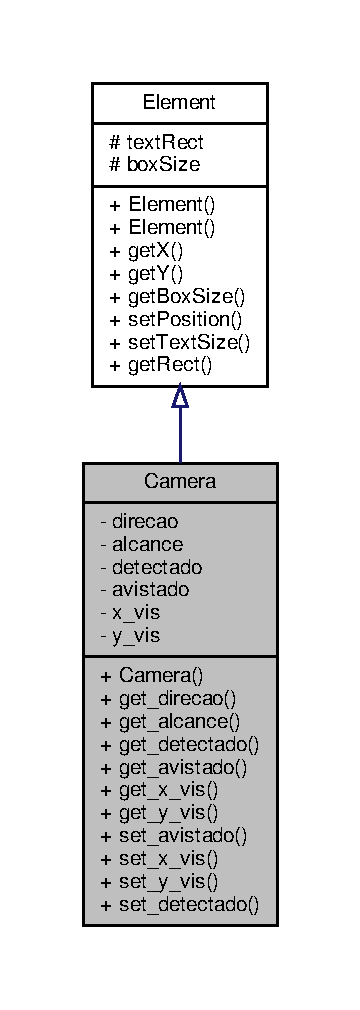
\includegraphics[width=173pt]{classCamera__inherit__graph}
\end{center}
\end{figure}


Collaboration diagram for Camera\+:
\nopagebreak
\begin{figure}[H]
\begin{center}
\leavevmode
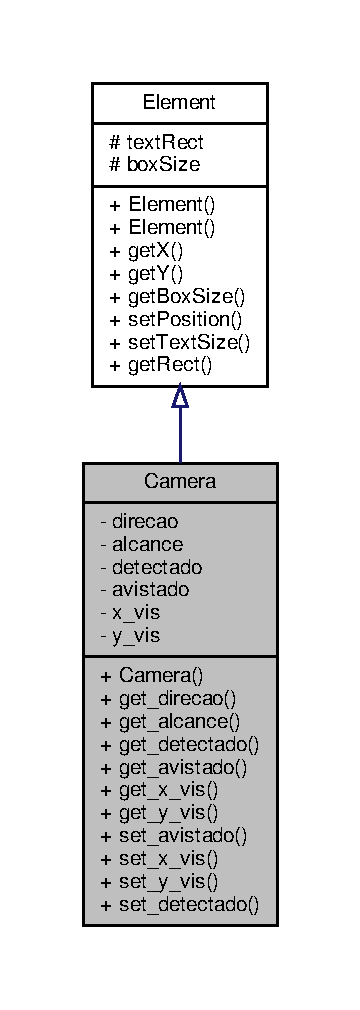
\includegraphics[width=173pt]{classCamera__coll__graph}
\end{center}
\end{figure}
\subsection*{Public Member Functions}
\begin{DoxyCompactItemize}
\item 
\hyperlink{classCamera_a297e1aba987f8418a355522e5a8b2f77}{Camera} (int \hyperlink{classCamera_a82594c03b409a1670e19f317e7d0e343}{direcao}, int \hyperlink{classCamera_a310e25ede9cb3f797c18fcecd7fef8fd}{alcance}, int x, int y)
\item 
int \hyperlink{classCamera_afd13cc91a3ce9a4d4d6b6dbb622ce7a4}{get\+\_\+direcao} ()
\item 
int \hyperlink{classCamera_a4603e48179e827b04679fce1f485dde1}{get\+\_\+alcance} ()
\item 
int \hyperlink{classCamera_a3b6202883eadc2e3b94f4cd1a2929111}{get\+\_\+detectado} ()
\item 
int \hyperlink{classCamera_a9a87643bf6bde3ca94b8f51f66e85574}{get\+\_\+avistado} ()
\item 
int \hyperlink{classCamera_a7b38e3e530865054f4425add99421f96}{get\+\_\+x\+\_\+vis} ()
\item 
int \hyperlink{classCamera_ad4ed7f3d1e12fc637ae8bbe9fad08430}{get\+\_\+y\+\_\+vis} ()
\item 
void \hyperlink{classCamera_a8f9f20cce133ec8f429f56e805ba1510}{set\+\_\+avistado} (int \hyperlink{classCamera_a2a0363d549c23561ba3c31e96244e00a}{avistado})
\item 
void \hyperlink{classCamera_abf6eb324c8d3900835e542a5ff5f9d43}{set\+\_\+x\+\_\+vis} (int \hyperlink{classCamera_ab817fd4f5ccb70d3d90b07fa4334c70b}{x\+\_\+vis})
\item 
void \hyperlink{classCamera_aea3c7f010360c4fe13ac738be2ea9027}{set\+\_\+y\+\_\+vis} (int \hyperlink{classCamera_a52e161a09b8e26feb580cc1740abcdad}{y\+\_\+vis})
\item 
void \hyperlink{classCamera_a809224178bedeb0b951891f91c0a5f58}{set\+\_\+detectado} (int \hyperlink{classCamera_a07b38e39acc6d3f808a27f0ddf2c79e2}{detectado})
\end{DoxyCompactItemize}
\subsection*{Private Attributes}
\begin{DoxyCompactItemize}
\item 
int \hyperlink{classCamera_a82594c03b409a1670e19f317e7d0e343}{direcao}
\item 
int \hyperlink{classCamera_a310e25ede9cb3f797c18fcecd7fef8fd}{alcance}
\item 
int \hyperlink{classCamera_a07b38e39acc6d3f808a27f0ddf2c79e2}{detectado}
\item 
int \hyperlink{classCamera_a2a0363d549c23561ba3c31e96244e00a}{avistado}
\item 
int \hyperlink{classCamera_ab817fd4f5ccb70d3d90b07fa4334c70b}{x\+\_\+vis}
\item 
int \hyperlink{classCamera_a52e161a09b8e26feb580cc1740abcdad}{y\+\_\+vis}
\end{DoxyCompactItemize}
\subsection*{Additional Inherited Members}


\subsection{Constructor \& Destructor Documentation}
\mbox{\Hypertarget{classCamera_a297e1aba987f8418a355522e5a8b2f77}\label{classCamera_a297e1aba987f8418a355522e5a8b2f77}} 
\index{Camera@{Camera}!Camera@{Camera}}
\index{Camera@{Camera}!Camera@{Camera}}
\subsubsection{\texorpdfstring{Camera()}{Camera()}}
{\footnotesize\ttfamily Camera\+::\+Camera (\begin{DoxyParamCaption}\item[{int}]{direcao,  }\item[{int}]{alcance,  }\item[{int}]{x,  }\item[{int}]{y }\end{DoxyParamCaption})}



\subsection{Member Function Documentation}
\mbox{\Hypertarget{classCamera_a4603e48179e827b04679fce1f485dde1}\label{classCamera_a4603e48179e827b04679fce1f485dde1}} 
\index{Camera@{Camera}!get\+\_\+alcance@{get\+\_\+alcance}}
\index{get\+\_\+alcance@{get\+\_\+alcance}!Camera@{Camera}}
\subsubsection{\texorpdfstring{get\+\_\+alcance()}{get\_alcance()}}
{\footnotesize\ttfamily int Camera\+::get\+\_\+alcance (\begin{DoxyParamCaption}{ }\end{DoxyParamCaption})}

\mbox{\Hypertarget{classCamera_a9a87643bf6bde3ca94b8f51f66e85574}\label{classCamera_a9a87643bf6bde3ca94b8f51f66e85574}} 
\index{Camera@{Camera}!get\+\_\+avistado@{get\+\_\+avistado}}
\index{get\+\_\+avistado@{get\+\_\+avistado}!Camera@{Camera}}
\subsubsection{\texorpdfstring{get\+\_\+avistado()}{get\_avistado()}}
{\footnotesize\ttfamily int Camera\+::get\+\_\+avistado (\begin{DoxyParamCaption}{ }\end{DoxyParamCaption})}

\mbox{\Hypertarget{classCamera_a3b6202883eadc2e3b94f4cd1a2929111}\label{classCamera_a3b6202883eadc2e3b94f4cd1a2929111}} 
\index{Camera@{Camera}!get\+\_\+detectado@{get\+\_\+detectado}}
\index{get\+\_\+detectado@{get\+\_\+detectado}!Camera@{Camera}}
\subsubsection{\texorpdfstring{get\+\_\+detectado()}{get\_detectado()}}
{\footnotesize\ttfamily int Camera\+::get\+\_\+detectado (\begin{DoxyParamCaption}{ }\end{DoxyParamCaption})}

\mbox{\Hypertarget{classCamera_afd13cc91a3ce9a4d4d6b6dbb622ce7a4}\label{classCamera_afd13cc91a3ce9a4d4d6b6dbb622ce7a4}} 
\index{Camera@{Camera}!get\+\_\+direcao@{get\+\_\+direcao}}
\index{get\+\_\+direcao@{get\+\_\+direcao}!Camera@{Camera}}
\subsubsection{\texorpdfstring{get\+\_\+direcao()}{get\_direcao()}}
{\footnotesize\ttfamily int Camera\+::get\+\_\+direcao (\begin{DoxyParamCaption}{ }\end{DoxyParamCaption})}

\mbox{\Hypertarget{classCamera_a7b38e3e530865054f4425add99421f96}\label{classCamera_a7b38e3e530865054f4425add99421f96}} 
\index{Camera@{Camera}!get\+\_\+x\+\_\+vis@{get\+\_\+x\+\_\+vis}}
\index{get\+\_\+x\+\_\+vis@{get\+\_\+x\+\_\+vis}!Camera@{Camera}}
\subsubsection{\texorpdfstring{get\+\_\+x\+\_\+vis()}{get\_x\_vis()}}
{\footnotesize\ttfamily int Camera\+::get\+\_\+x\+\_\+vis (\begin{DoxyParamCaption}{ }\end{DoxyParamCaption})}

\mbox{\Hypertarget{classCamera_ad4ed7f3d1e12fc637ae8bbe9fad08430}\label{classCamera_ad4ed7f3d1e12fc637ae8bbe9fad08430}} 
\index{Camera@{Camera}!get\+\_\+y\+\_\+vis@{get\+\_\+y\+\_\+vis}}
\index{get\+\_\+y\+\_\+vis@{get\+\_\+y\+\_\+vis}!Camera@{Camera}}
\subsubsection{\texorpdfstring{get\+\_\+y\+\_\+vis()}{get\_y\_vis()}}
{\footnotesize\ttfamily int Camera\+::get\+\_\+y\+\_\+vis (\begin{DoxyParamCaption}{ }\end{DoxyParamCaption})}

\mbox{\Hypertarget{classCamera_a8f9f20cce133ec8f429f56e805ba1510}\label{classCamera_a8f9f20cce133ec8f429f56e805ba1510}} 
\index{Camera@{Camera}!set\+\_\+avistado@{set\+\_\+avistado}}
\index{set\+\_\+avistado@{set\+\_\+avistado}!Camera@{Camera}}
\subsubsection{\texorpdfstring{set\+\_\+avistado()}{set\_avistado()}}
{\footnotesize\ttfamily void Camera\+::set\+\_\+avistado (\begin{DoxyParamCaption}\item[{int}]{avistado }\end{DoxyParamCaption})}

\mbox{\Hypertarget{classCamera_a809224178bedeb0b951891f91c0a5f58}\label{classCamera_a809224178bedeb0b951891f91c0a5f58}} 
\index{Camera@{Camera}!set\+\_\+detectado@{set\+\_\+detectado}}
\index{set\+\_\+detectado@{set\+\_\+detectado}!Camera@{Camera}}
\subsubsection{\texorpdfstring{set\+\_\+detectado()}{set\_detectado()}}
{\footnotesize\ttfamily void Camera\+::set\+\_\+detectado (\begin{DoxyParamCaption}\item[{int}]{detectado }\end{DoxyParamCaption})}

\mbox{\Hypertarget{classCamera_abf6eb324c8d3900835e542a5ff5f9d43}\label{classCamera_abf6eb324c8d3900835e542a5ff5f9d43}} 
\index{Camera@{Camera}!set\+\_\+x\+\_\+vis@{set\+\_\+x\+\_\+vis}}
\index{set\+\_\+x\+\_\+vis@{set\+\_\+x\+\_\+vis}!Camera@{Camera}}
\subsubsection{\texorpdfstring{set\+\_\+x\+\_\+vis()}{set\_x\_vis()}}
{\footnotesize\ttfamily void Camera\+::set\+\_\+x\+\_\+vis (\begin{DoxyParamCaption}\item[{int}]{x\+\_\+vis }\end{DoxyParamCaption})}

\mbox{\Hypertarget{classCamera_aea3c7f010360c4fe13ac738be2ea9027}\label{classCamera_aea3c7f010360c4fe13ac738be2ea9027}} 
\index{Camera@{Camera}!set\+\_\+y\+\_\+vis@{set\+\_\+y\+\_\+vis}}
\index{set\+\_\+y\+\_\+vis@{set\+\_\+y\+\_\+vis}!Camera@{Camera}}
\subsubsection{\texorpdfstring{set\+\_\+y\+\_\+vis()}{set\_y\_vis()}}
{\footnotesize\ttfamily void Camera\+::set\+\_\+y\+\_\+vis (\begin{DoxyParamCaption}\item[{int}]{y\+\_\+vis }\end{DoxyParamCaption})}



\subsection{Member Data Documentation}
\mbox{\Hypertarget{classCamera_a310e25ede9cb3f797c18fcecd7fef8fd}\label{classCamera_a310e25ede9cb3f797c18fcecd7fef8fd}} 
\index{Camera@{Camera}!alcance@{alcance}}
\index{alcance@{alcance}!Camera@{Camera}}
\subsubsection{\texorpdfstring{alcance}{alcance}}
{\footnotesize\ttfamily int Camera\+::alcance\hspace{0.3cm}{\ttfamily [private]}}

\mbox{\Hypertarget{classCamera_a2a0363d549c23561ba3c31e96244e00a}\label{classCamera_a2a0363d549c23561ba3c31e96244e00a}} 
\index{Camera@{Camera}!avistado@{avistado}}
\index{avistado@{avistado}!Camera@{Camera}}
\subsubsection{\texorpdfstring{avistado}{avistado}}
{\footnotesize\ttfamily int Camera\+::avistado\hspace{0.3cm}{\ttfamily [private]}}

\mbox{\Hypertarget{classCamera_a07b38e39acc6d3f808a27f0ddf2c79e2}\label{classCamera_a07b38e39acc6d3f808a27f0ddf2c79e2}} 
\index{Camera@{Camera}!detectado@{detectado}}
\index{detectado@{detectado}!Camera@{Camera}}
\subsubsection{\texorpdfstring{detectado}{detectado}}
{\footnotesize\ttfamily int Camera\+::detectado\hspace{0.3cm}{\ttfamily [private]}}

\mbox{\Hypertarget{classCamera_a82594c03b409a1670e19f317e7d0e343}\label{classCamera_a82594c03b409a1670e19f317e7d0e343}} 
\index{Camera@{Camera}!direcao@{direcao}}
\index{direcao@{direcao}!Camera@{Camera}}
\subsubsection{\texorpdfstring{direcao}{direcao}}
{\footnotesize\ttfamily int Camera\+::direcao\hspace{0.3cm}{\ttfamily [private]}}

\mbox{\Hypertarget{classCamera_ab817fd4f5ccb70d3d90b07fa4334c70b}\label{classCamera_ab817fd4f5ccb70d3d90b07fa4334c70b}} 
\index{Camera@{Camera}!x\+\_\+vis@{x\+\_\+vis}}
\index{x\+\_\+vis@{x\+\_\+vis}!Camera@{Camera}}
\subsubsection{\texorpdfstring{x\+\_\+vis}{x\_vis}}
{\footnotesize\ttfamily int Camera\+::x\+\_\+vis\hspace{0.3cm}{\ttfamily [private]}}

\mbox{\Hypertarget{classCamera_a52e161a09b8e26feb580cc1740abcdad}\label{classCamera_a52e161a09b8e26feb580cc1740abcdad}} 
\index{Camera@{Camera}!y\+\_\+vis@{y\+\_\+vis}}
\index{y\+\_\+vis@{y\+\_\+vis}!Camera@{Camera}}
\subsubsection{\texorpdfstring{y\+\_\+vis}{y\_vis}}
{\footnotesize\ttfamily int Camera\+::y\+\_\+vis\hspace{0.3cm}{\ttfamily [private]}}



The documentation for this class was generated from the following files\+:\begin{DoxyCompactItemize}
\item 
include/\hyperlink{camera_8h}{camera.\+h}\item 
src/\hyperlink{camera_8cpp}{camera.\+cpp}\end{DoxyCompactItemize}

\hypertarget{classCamera__controller}{}\section{Camera\+\_\+controller Class Reference}
\label{classCamera__controller}\index{Camera\+\_\+controller@{Camera\+\_\+controller}}


{\ttfamily \#include $<$camera\+\_\+controller.\+h$>$}



Collaboration diagram for Camera\+\_\+controller\+:
\nopagebreak
\begin{figure}[H]
\begin{center}
\leavevmode
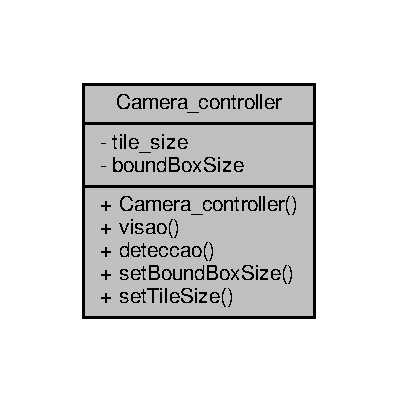
\includegraphics[width=191pt]{classCamera__controller__coll__graph}
\end{center}
\end{figure}
\subsection*{Public Member Functions}
\begin{DoxyCompactItemize}
\item 
\hyperlink{classCamera__controller_aa086aceef7d7548429d2023f333e3b19}{Camera\+\_\+controller} ()=default
\item 
void \hyperlink{classCamera__controller_a0d2df9cb25e3a63cd76fe8e0b2a9686d}{visao} (\hyperlink{classMap}{Map} \&mapa, \hyperlink{classCamera}{Camera} \&camera, \hyperlink{classPlayer}{Player} \&jogador)
\item 
void \hyperlink{classCamera__controller_a039d613f59cd15c4ea2a0493ca47701b}{deteccao} (\hyperlink{classMap}{Map} \&mapa, \hyperlink{classCamera}{Camera} \&camera, \hyperlink{classPlayer}{Player} \&jogador)
\item 
void \hyperlink{classCamera__controller_a15d8ce3924d5a274db49cccc2794536d}{set\+Bound\+Box\+Size} (int s)
\item 
void \hyperlink{classCamera__controller_a1e5255b02b3bc54d7b4ac92830f8f41c}{set\+Tile\+Size} (int s)
\end{DoxyCompactItemize}
\subsection*{Private Attributes}
\begin{DoxyCompactItemize}
\item 
int \hyperlink{classCamera__controller_ae2f8c96d3f03011a11cdcb4c8016fcef}{tile\+\_\+size} = 72
\item 
int \hyperlink{classCamera__controller_a3932aa7665e9edc834373a3e2f42f0e1}{bound\+Box\+Size} = 0
\end{DoxyCompactItemize}


\subsection{Constructor \& Destructor Documentation}
\mbox{\Hypertarget{classCamera__controller_aa086aceef7d7548429d2023f333e3b19}\label{classCamera__controller_aa086aceef7d7548429d2023f333e3b19}} 
\index{Camera\+\_\+controller@{Camera\+\_\+controller}!Camera\+\_\+controller@{Camera\+\_\+controller}}
\index{Camera\+\_\+controller@{Camera\+\_\+controller}!Camera\+\_\+controller@{Camera\+\_\+controller}}
\subsubsection{\texorpdfstring{Camera\+\_\+controller()}{Camera\_controller()}}
{\footnotesize\ttfamily Camera\+\_\+controller\+::\+Camera\+\_\+controller (\begin{DoxyParamCaption}{ }\end{DoxyParamCaption})\hspace{0.3cm}{\ttfamily [default]}}



\subsection{Member Function Documentation}
\mbox{\Hypertarget{classCamera__controller_a039d613f59cd15c4ea2a0493ca47701b}\label{classCamera__controller_a039d613f59cd15c4ea2a0493ca47701b}} 
\index{Camera\+\_\+controller@{Camera\+\_\+controller}!deteccao@{deteccao}}
\index{deteccao@{deteccao}!Camera\+\_\+controller@{Camera\+\_\+controller}}
\subsubsection{\texorpdfstring{deteccao()}{deteccao()}}
{\footnotesize\ttfamily void Camera\+\_\+controller\+::deteccao (\begin{DoxyParamCaption}\item[{\hyperlink{classMap}{Map} \&}]{mapa,  }\item[{\hyperlink{classCamera}{Camera} \&}]{camera,  }\item[{\hyperlink{classPlayer}{Player} \&}]{jogador }\end{DoxyParamCaption})}

\mbox{\Hypertarget{classCamera__controller_a15d8ce3924d5a274db49cccc2794536d}\label{classCamera__controller_a15d8ce3924d5a274db49cccc2794536d}} 
\index{Camera\+\_\+controller@{Camera\+\_\+controller}!set\+Bound\+Box\+Size@{set\+Bound\+Box\+Size}}
\index{set\+Bound\+Box\+Size@{set\+Bound\+Box\+Size}!Camera\+\_\+controller@{Camera\+\_\+controller}}
\subsubsection{\texorpdfstring{set\+Bound\+Box\+Size()}{setBoundBoxSize()}}
{\footnotesize\ttfamily void Camera\+\_\+controller\+::set\+Bound\+Box\+Size (\begin{DoxyParamCaption}\item[{int}]{s }\end{DoxyParamCaption})}

\mbox{\Hypertarget{classCamera__controller_a1e5255b02b3bc54d7b4ac92830f8f41c}\label{classCamera__controller_a1e5255b02b3bc54d7b4ac92830f8f41c}} 
\index{Camera\+\_\+controller@{Camera\+\_\+controller}!set\+Tile\+Size@{set\+Tile\+Size}}
\index{set\+Tile\+Size@{set\+Tile\+Size}!Camera\+\_\+controller@{Camera\+\_\+controller}}
\subsubsection{\texorpdfstring{set\+Tile\+Size()}{setTileSize()}}
{\footnotesize\ttfamily void Camera\+\_\+controller\+::set\+Tile\+Size (\begin{DoxyParamCaption}\item[{int}]{s }\end{DoxyParamCaption})}

\mbox{\Hypertarget{classCamera__controller_a0d2df9cb25e3a63cd76fe8e0b2a9686d}\label{classCamera__controller_a0d2df9cb25e3a63cd76fe8e0b2a9686d}} 
\index{Camera\+\_\+controller@{Camera\+\_\+controller}!visao@{visao}}
\index{visao@{visao}!Camera\+\_\+controller@{Camera\+\_\+controller}}
\subsubsection{\texorpdfstring{visao()}{visao()}}
{\footnotesize\ttfamily void Camera\+\_\+controller\+::visao (\begin{DoxyParamCaption}\item[{\hyperlink{classMap}{Map} \&}]{mapa,  }\item[{\hyperlink{classCamera}{Camera} \&}]{camera,  }\item[{\hyperlink{classPlayer}{Player} \&}]{jogador }\end{DoxyParamCaption})}



\subsection{Member Data Documentation}
\mbox{\Hypertarget{classCamera__controller_a3932aa7665e9edc834373a3e2f42f0e1}\label{classCamera__controller_a3932aa7665e9edc834373a3e2f42f0e1}} 
\index{Camera\+\_\+controller@{Camera\+\_\+controller}!bound\+Box\+Size@{bound\+Box\+Size}}
\index{bound\+Box\+Size@{bound\+Box\+Size}!Camera\+\_\+controller@{Camera\+\_\+controller}}
\subsubsection{\texorpdfstring{bound\+Box\+Size}{boundBoxSize}}
{\footnotesize\ttfamily int Camera\+\_\+controller\+::bound\+Box\+Size = 0\hspace{0.3cm}{\ttfamily [private]}}

\mbox{\Hypertarget{classCamera__controller_ae2f8c96d3f03011a11cdcb4c8016fcef}\label{classCamera__controller_ae2f8c96d3f03011a11cdcb4c8016fcef}} 
\index{Camera\+\_\+controller@{Camera\+\_\+controller}!tile\+\_\+size@{tile\+\_\+size}}
\index{tile\+\_\+size@{tile\+\_\+size}!Camera\+\_\+controller@{Camera\+\_\+controller}}
\subsubsection{\texorpdfstring{tile\+\_\+size}{tile\_size}}
{\footnotesize\ttfamily int Camera\+\_\+controller\+::tile\+\_\+size = 72\hspace{0.3cm}{\ttfamily [private]}}



The documentation for this class was generated from the following files\+:\begin{DoxyCompactItemize}
\item 
include/\hyperlink{camera__controller_8h}{camera\+\_\+controller.\+h}\item 
src/\hyperlink{camera__controller_8cpp}{camera\+\_\+controller.\+cpp}\end{DoxyCompactItemize}

\hypertarget{classcollisionController}{}\section{collision\+Controller Class Reference}
\label{classcollisionController}\index{collision\+Controller@{collision\+Controller}}


Controle de Colisão.  




{\ttfamily \#include $<$collision\+Controller.\+h$>$}



Collaboration diagram for collision\+Controller\+:
\nopagebreak
\begin{figure}[H]
\begin{center}
\leavevmode
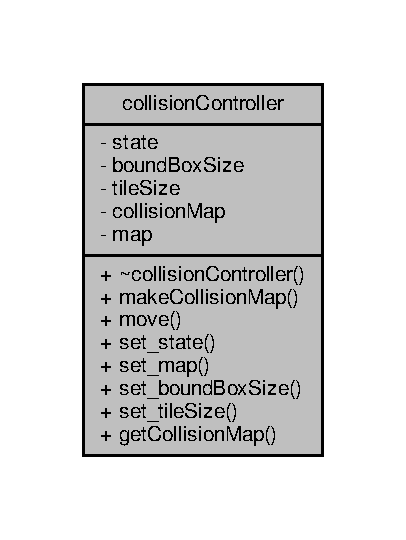
\includegraphics[width=195pt]{classcollisionController__coll__graph}
\end{center}
\end{figure}
\subsection*{Public Member Functions}
\begin{DoxyCompactItemize}
\item 
\hyperlink{classcollisionController_a602c73073a3f2f44a8dc65952113f5de}{$\sim$collision\+Controller} ()
\item 
void \hyperlink{classcollisionController_aac25970400c5d905dbf60e69da3720c5}{make\+Collision\+Map} ()
\item 
void \hyperlink{classcollisionController_ad08a8b7f1bc6f803a8875a89ac194bba}{move} (\hyperlink{classPlayer}{Player} \&obj)
\item 
void \hyperlink{classcollisionController_ab92231229dbb6786429137147b4d232b}{set\+\_\+state} (const Uint8 $\ast$\hyperlink{classcollisionController_a5957b53016d027965bf98cf391df28cb}{state})
\item 
void \hyperlink{classcollisionController_aee7db17044f602c0b8a553012540480b}{set\+\_\+map} (std\+::shared\+\_\+ptr$<$ \hyperlink{classMap}{Map} $>$ \hyperlink{classcollisionController_a9624b45dd5e3ba5317291f96e68dcf76}{map})
\item 
void \hyperlink{classcollisionController_a0b59127f63d5caeeb5fa3c573853c8e7}{set\+\_\+bound\+Box\+Size} (int size)
\item 
void \hyperlink{classcollisionController_a025770daba1c75e9479c2375a6543edf}{set\+\_\+tile\+Size} (int size)
\item 
int $\ast$$\ast$ \hyperlink{classcollisionController_adcba90a401d69ebeb270ae0b92b9c335}{get\+Collision\+Map} ()
\end{DoxyCompactItemize}
\subsection*{Private Attributes}
\begin{DoxyCompactItemize}
\item 
const Uint8 $\ast$ \hyperlink{classcollisionController_a5957b53016d027965bf98cf391df28cb}{state} = N\+U\+LL
\item 
int \hyperlink{classcollisionController_a6624f68ec989fb6cce2a6b9f46c15dc3}{bound\+Box\+Size} = 0
\item 
int \hyperlink{classcollisionController_a9a844a9c3873ea03ec04dd382040167c}{tile\+Size} = 0
\item 
int $\ast$$\ast$ \hyperlink{classcollisionController_a71bbc836de2531fa217d46f37f501e71}{collision\+Map} = N\+U\+LL
\item 
std\+::shared\+\_\+ptr$<$ \hyperlink{classMap}{Map} $>$ \hyperlink{classcollisionController_a9624b45dd5e3ba5317291f96e68dcf76}{map}
\end{DoxyCompactItemize}


\subsection{Detailed Description}
Controle de Colisão. 

Controla movimentos e colisão. Atualiza o sprite da animação do jogador. 

\subsection{Constructor \& Destructor Documentation}
\mbox{\Hypertarget{classcollisionController_a602c73073a3f2f44a8dc65952113f5de}\label{classcollisionController_a602c73073a3f2f44a8dc65952113f5de}} 
\index{collision\+Controller@{collision\+Controller}!````~collision\+Controller@{$\sim$collision\+Controller}}
\index{````~collision\+Controller@{$\sim$collision\+Controller}!collision\+Controller@{collision\+Controller}}
\subsubsection{\texorpdfstring{$\sim$collision\+Controller()}{~collisionController()}}
{\footnotesize\ttfamily collision\+Controller\+::$\sim$collision\+Controller (\begin{DoxyParamCaption}{ }\end{DoxyParamCaption})}

Desaloca mapa de colisão 

\subsection{Member Function Documentation}
\mbox{\Hypertarget{classcollisionController_adcba90a401d69ebeb270ae0b92b9c335}\label{classcollisionController_adcba90a401d69ebeb270ae0b92b9c335}} 
\index{collision\+Controller@{collision\+Controller}!get\+Collision\+Map@{get\+Collision\+Map}}
\index{get\+Collision\+Map@{get\+Collision\+Map}!collision\+Controller@{collision\+Controller}}
\subsubsection{\texorpdfstring{get\+Collision\+Map()}{getCollisionMap()}}
{\footnotesize\ttfamily int $\ast$$\ast$ collision\+Controller\+::get\+Collision\+Map (\begin{DoxyParamCaption}{ }\end{DoxyParamCaption})}

\mbox{\Hypertarget{classcollisionController_aac25970400c5d905dbf60e69da3720c5}\label{classcollisionController_aac25970400c5d905dbf60e69da3720c5}} 
\index{collision\+Controller@{collision\+Controller}!make\+Collision\+Map@{make\+Collision\+Map}}
\index{make\+Collision\+Map@{make\+Collision\+Map}!collision\+Controller@{collision\+Controller}}
\subsubsection{\texorpdfstring{make\+Collision\+Map()}{makeCollisionMap()}}
{\footnotesize\ttfamily void collision\+Controller\+::make\+Collision\+Map (\begin{DoxyParamCaption}{ }\end{DoxyParamCaption})}

Gera mapa de colisão a partir do dicionário do mapa \mbox{\Hypertarget{classcollisionController_ad08a8b7f1bc6f803a8875a89ac194bba}\label{classcollisionController_ad08a8b7f1bc6f803a8875a89ac194bba}} 
\index{collision\+Controller@{collision\+Controller}!move@{move}}
\index{move@{move}!collision\+Controller@{collision\+Controller}}
\subsubsection{\texorpdfstring{move()}{move()}}
{\footnotesize\ttfamily void collision\+Controller\+::move (\begin{DoxyParamCaption}\item[{\hyperlink{classPlayer}{Player} \&}]{obj }\end{DoxyParamCaption})}

Move o player controlando a colisão 
\begin{DoxyParams}{Parameters}
{\em obj} & \hyperlink{classPlayer}{Player} a ser movido \\
\hline
\end{DoxyParams}
\mbox{\Hypertarget{classcollisionController_a0b59127f63d5caeeb5fa3c573853c8e7}\label{classcollisionController_a0b59127f63d5caeeb5fa3c573853c8e7}} 
\index{collision\+Controller@{collision\+Controller}!set\+\_\+bound\+Box\+Size@{set\+\_\+bound\+Box\+Size}}
\index{set\+\_\+bound\+Box\+Size@{set\+\_\+bound\+Box\+Size}!collision\+Controller@{collision\+Controller}}
\subsubsection{\texorpdfstring{set\+\_\+bound\+Box\+Size()}{set\_boundBoxSize()}}
{\footnotesize\ttfamily void collision\+Controller\+::set\+\_\+bound\+Box\+Size (\begin{DoxyParamCaption}\item[{int}]{size }\end{DoxyParamCaption})}

\mbox{\Hypertarget{classcollisionController_aee7db17044f602c0b8a553012540480b}\label{classcollisionController_aee7db17044f602c0b8a553012540480b}} 
\index{collision\+Controller@{collision\+Controller}!set\+\_\+map@{set\+\_\+map}}
\index{set\+\_\+map@{set\+\_\+map}!collision\+Controller@{collision\+Controller}}
\subsubsection{\texorpdfstring{set\+\_\+map()}{set\_map()}}
{\footnotesize\ttfamily void collision\+Controller\+::set\+\_\+map (\begin{DoxyParamCaption}\item[{std\+::shared\+\_\+ptr$<$ \hyperlink{classMap}{Map} $>$}]{map }\end{DoxyParamCaption})}

\mbox{\Hypertarget{classcollisionController_ab92231229dbb6786429137147b4d232b}\label{classcollisionController_ab92231229dbb6786429137147b4d232b}} 
\index{collision\+Controller@{collision\+Controller}!set\+\_\+state@{set\+\_\+state}}
\index{set\+\_\+state@{set\+\_\+state}!collision\+Controller@{collision\+Controller}}
\subsubsection{\texorpdfstring{set\+\_\+state()}{set\_state()}}
{\footnotesize\ttfamily void collision\+Controller\+::set\+\_\+state (\begin{DoxyParamCaption}\item[{const Uint8 $\ast$}]{state }\end{DoxyParamCaption})}

\mbox{\Hypertarget{classcollisionController_a025770daba1c75e9479c2375a6543edf}\label{classcollisionController_a025770daba1c75e9479c2375a6543edf}} 
\index{collision\+Controller@{collision\+Controller}!set\+\_\+tile\+Size@{set\+\_\+tile\+Size}}
\index{set\+\_\+tile\+Size@{set\+\_\+tile\+Size}!collision\+Controller@{collision\+Controller}}
\subsubsection{\texorpdfstring{set\+\_\+tile\+Size()}{set\_tileSize()}}
{\footnotesize\ttfamily void collision\+Controller\+::set\+\_\+tile\+Size (\begin{DoxyParamCaption}\item[{int}]{size }\end{DoxyParamCaption})}



\subsection{Member Data Documentation}
\mbox{\Hypertarget{classcollisionController_a6624f68ec989fb6cce2a6b9f46c15dc3}\label{classcollisionController_a6624f68ec989fb6cce2a6b9f46c15dc3}} 
\index{collision\+Controller@{collision\+Controller}!bound\+Box\+Size@{bound\+Box\+Size}}
\index{bound\+Box\+Size@{bound\+Box\+Size}!collision\+Controller@{collision\+Controller}}
\subsubsection{\texorpdfstring{bound\+Box\+Size}{boundBoxSize}}
{\footnotesize\ttfamily int collision\+Controller\+::bound\+Box\+Size = 0\hspace{0.3cm}{\ttfamily [private]}}

\mbox{\Hypertarget{classcollisionController_a71bbc836de2531fa217d46f37f501e71}\label{classcollisionController_a71bbc836de2531fa217d46f37f501e71}} 
\index{collision\+Controller@{collision\+Controller}!collision\+Map@{collision\+Map}}
\index{collision\+Map@{collision\+Map}!collision\+Controller@{collision\+Controller}}
\subsubsection{\texorpdfstring{collision\+Map}{collisionMap}}
{\footnotesize\ttfamily int$\ast$$\ast$ collision\+Controller\+::collision\+Map = N\+U\+LL\hspace{0.3cm}{\ttfamily [private]}}

Mapa de colisão \mbox{\Hypertarget{classcollisionController_a9624b45dd5e3ba5317291f96e68dcf76}\label{classcollisionController_a9624b45dd5e3ba5317291f96e68dcf76}} 
\index{collision\+Controller@{collision\+Controller}!map@{map}}
\index{map@{map}!collision\+Controller@{collision\+Controller}}
\subsubsection{\texorpdfstring{map}{map}}
{\footnotesize\ttfamily std\+::shared\+\_\+ptr$<$\hyperlink{classMap}{Map}$>$ collision\+Controller\+::map\hspace{0.3cm}{\ttfamily [private]}}

Ponteiro para mapa \mbox{\Hypertarget{classcollisionController_a5957b53016d027965bf98cf391df28cb}\label{classcollisionController_a5957b53016d027965bf98cf391df28cb}} 
\index{collision\+Controller@{collision\+Controller}!state@{state}}
\index{state@{state}!collision\+Controller@{collision\+Controller}}
\subsubsection{\texorpdfstring{state}{state}}
{\footnotesize\ttfamily const Uint8$\ast$ collision\+Controller\+::state = N\+U\+LL\hspace{0.3cm}{\ttfamily [private]}}

Estado do Teclado \mbox{\Hypertarget{classcollisionController_a9a844a9c3873ea03ec04dd382040167c}\label{classcollisionController_a9a844a9c3873ea03ec04dd382040167c}} 
\index{collision\+Controller@{collision\+Controller}!tile\+Size@{tile\+Size}}
\index{tile\+Size@{tile\+Size}!collision\+Controller@{collision\+Controller}}
\subsubsection{\texorpdfstring{tile\+Size}{tileSize}}
{\footnotesize\ttfamily int collision\+Controller\+::tile\+Size = 0\hspace{0.3cm}{\ttfamily [private]}}



The documentation for this class was generated from the following files\+:\begin{DoxyCompactItemize}
\item 
include/\hyperlink{collisionController_8h}{collision\+Controller.\+h}\item 
src/\hyperlink{collisionController_8cpp}{collision\+Controller.\+cpp}\end{DoxyCompactItemize}

\hypertarget{classController}{}\section{Controller Class Reference}
\label{classController}\index{Controller@{Controller}}


Classe para o controller.  




{\ttfamily \#include $<$controller.\+h$>$}



Collaboration diagram for Controller\+:
\nopagebreak
\begin{figure}[H]
\begin{center}
\leavevmode
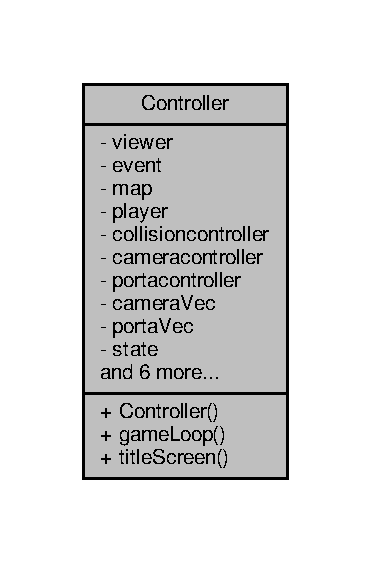
\includegraphics[width=178pt]{classController__coll__graph}
\end{center}
\end{figure}
\subsection*{Public Member Functions}
\begin{DoxyCompactItemize}
\item 
\hyperlink{classController_a95c56822d667e94b031451729ce069a9}{Controller} ()
\begin{DoxyCompactList}\small\item\em Construtor do \hyperlink{classController}{Controller}. \end{DoxyCompactList}\item 
void \hyperlink{classController_a31ede2d3d9dba71913635bfe025b443d}{game\+Loop} ()
\begin{DoxyCompactList}\small\item\em Loop principal. \end{DoxyCompactList}\item 
void \hyperlink{classController_a18960c9e5f51f4844d51d27fb394ff85}{title\+Screen} ()
\begin{DoxyCompactList}\small\item\em Tela Principal. \end{DoxyCompactList}\end{DoxyCompactItemize}
\subsection*{Private Attributes}
\begin{DoxyCompactItemize}
\item 
std\+::shared\+\_\+ptr$<$ \hyperlink{classViewer}{Viewer} $>$ \hyperlink{classController_a9a290ffa5eeaf96a42daa9a68dc501ff}{viewer}
\item 
std\+::shared\+\_\+ptr$<$ \hyperlink{classEventos}{Eventos} $>$ \hyperlink{classController_a4f7ee884b34086ac959074caeb3b5107}{event}
\item 
std\+::shared\+\_\+ptr$<$ \hyperlink{classMap}{Map} $>$ \hyperlink{classController_a48cd1eac2b8cf98947433f580aa72feb}{map}
\item 
std\+::shared\+\_\+ptr$<$ \hyperlink{classPlayer}{Player} $>$ \hyperlink{classController_a96a143b0a60e1429c60f5fae58326bb6}{player}
\item 
std\+::shared\+\_\+ptr$<$ \hyperlink{classcollisionController}{collision\+Controller} $>$ \hyperlink{classController_a94db10a8bbfe6ad62d893cb4589d48d1}{collisioncontroller}
\item 
std\+::shared\+\_\+ptr$<$ \hyperlink{classCamera__controller}{Camera\+\_\+controller} $>$ \hyperlink{classController_a0fff98a80ea67c6c500d4f06f0d11995}{cameracontroller}
\item 
std\+::shared\+\_\+ptr$<$ \hyperlink{classPorta__controller}{Porta\+\_\+controller} $>$ \hyperlink{classController_a0dbb09739500259753bd2340d54e031c}{portacontroller}
\item 
std\+::vector$<$ std\+::shared\+\_\+ptr$<$ \hyperlink{classCamera}{Camera} $>$ $>$ \hyperlink{classController_a44b8398dc1a926b7528e32288b9bb7cd}{camera\+Vec}
\item 
std\+::vector$<$ std\+::shared\+\_\+ptr$<$ \hyperlink{classPorta}{Porta} $>$ $>$ \hyperlink{classController_ab386b5e19c31282f0471e011b65393ae}{porta\+Vec}
\item 
const Uint8 $\ast$ \hyperlink{classController_a4e2c7234de84518990f047e5e3d2f35e}{state} = N\+U\+LL
\item 
bool \hyperlink{classController_aafde74afadbef3109d8af8c324f6cc44}{rodando} = true
\item 
S\+D\+L\+\_\+\+Event \hyperlink{classController_aff78b97e8a07364fd11317c50fb98f88}{evento}
\item 
int \hyperlink{classController_ace9ec6683586dc71ad011b5b364b353e}{porta\+Event\+Counter} = 0
\item 
int \hyperlink{classController_aa4a9bf69dacf847c848e14838838f272}{porta\+Go} = 0
\item 
int \hyperlink{classController_a1f75badb13e3132e0f390a8838c33ad5}{tile\+Size}
\item 
int \hyperlink{classController_afdb6115d8bbca2eb32d253e66ee0b105}{box\+Size}
\end{DoxyCompactItemize}


\subsection{Detailed Description}
Classe para o controller. 

\hyperlink{classController}{Controller} Principal. Responsável pelo loop principal do jogo. Guarda ponteiros para todos os objetos. 

\subsection{Constructor \& Destructor Documentation}
\mbox{\Hypertarget{classController_a95c56822d667e94b031451729ce069a9}\label{classController_a95c56822d667e94b031451729ce069a9}} 
\index{Controller@{Controller}!Controller@{Controller}}
\index{Controller@{Controller}!Controller@{Controller}}
\subsubsection{\texorpdfstring{Controller()}{Controller()}}
{\footnotesize\ttfamily Controller\+::\+Controller (\begin{DoxyParamCaption}{ }\end{DoxyParamCaption})}



Construtor do \hyperlink{classController}{Controller}. 

Aloca memória para os objetos principais. Configura objetos.

\begin{DoxyReturn}{Returns}
Nada (este é um construtor!) 
\end{DoxyReturn}


\subsection{Member Function Documentation}
\mbox{\Hypertarget{classController_a31ede2d3d9dba71913635bfe025b443d}\label{classController_a31ede2d3d9dba71913635bfe025b443d}} 
\index{Controller@{Controller}!game\+Loop@{game\+Loop}}
\index{game\+Loop@{game\+Loop}!Controller@{Controller}}
\subsubsection{\texorpdfstring{game\+Loop()}{gameLoop()}}
{\footnotesize\ttfamily void Controller\+::game\+Loop (\begin{DoxyParamCaption}{ }\end{DoxyParamCaption})}



Loop principal. 

Loop principal do jogo. Roda os controllers secundáros. \mbox{\Hypertarget{classController_a18960c9e5f51f4844d51d27fb394ff85}\label{classController_a18960c9e5f51f4844d51d27fb394ff85}} 
\index{Controller@{Controller}!title\+Screen@{title\+Screen}}
\index{title\+Screen@{title\+Screen}!Controller@{Controller}}
\subsubsection{\texorpdfstring{title\+Screen()}{titleScreen()}}
{\footnotesize\ttfamily void Controller\+::title\+Screen (\begin{DoxyParamCaption}{ }\end{DoxyParamCaption})}



Tela Principal. 

Renderiza a tela principal até que o jogador aperte espaço. 

\subsection{Member Data Documentation}
\mbox{\Hypertarget{classController_afdb6115d8bbca2eb32d253e66ee0b105}\label{classController_afdb6115d8bbca2eb32d253e66ee0b105}} 
\index{Controller@{Controller}!box\+Size@{box\+Size}}
\index{box\+Size@{box\+Size}!Controller@{Controller}}
\subsubsection{\texorpdfstring{box\+Size}{boxSize}}
{\footnotesize\ttfamily int Controller\+::box\+Size\hspace{0.3cm}{\ttfamily [private]}}

Tamanho do bounding box do Jogador \mbox{\Hypertarget{classController_a0fff98a80ea67c6c500d4f06f0d11995}\label{classController_a0fff98a80ea67c6c500d4f06f0d11995}} 
\index{Controller@{Controller}!cameracontroller@{cameracontroller}}
\index{cameracontroller@{cameracontroller}!Controller@{Controller}}
\subsubsection{\texorpdfstring{cameracontroller}{cameracontroller}}
{\footnotesize\ttfamily std\+::shared\+\_\+ptr$<$\hyperlink{classCamera__controller}{Camera\+\_\+controller}$>$ Controller\+::cameracontroller\hspace{0.3cm}{\ttfamily [private]}}

\mbox{\Hypertarget{classController_a44b8398dc1a926b7528e32288b9bb7cd}\label{classController_a44b8398dc1a926b7528e32288b9bb7cd}} 
\index{Controller@{Controller}!camera\+Vec@{camera\+Vec}}
\index{camera\+Vec@{camera\+Vec}!Controller@{Controller}}
\subsubsection{\texorpdfstring{camera\+Vec}{cameraVec}}
{\footnotesize\ttfamily std\+::vector$<$std\+::shared\+\_\+ptr$<$\hyperlink{classCamera}{Camera}$>$ $>$ Controller\+::camera\+Vec\hspace{0.3cm}{\ttfamily [private]}}

Guarda todas as cameras \mbox{\Hypertarget{classController_a94db10a8bbfe6ad62d893cb4589d48d1}\label{classController_a94db10a8bbfe6ad62d893cb4589d48d1}} 
\index{Controller@{Controller}!collisioncontroller@{collisioncontroller}}
\index{collisioncontroller@{collisioncontroller}!Controller@{Controller}}
\subsubsection{\texorpdfstring{collisioncontroller}{collisioncontroller}}
{\footnotesize\ttfamily std\+::shared\+\_\+ptr$<$\hyperlink{classcollisionController}{collision\+Controller}$>$ Controller\+::collisioncontroller\hspace{0.3cm}{\ttfamily [private]}}

\mbox{\Hypertarget{classController_a4f7ee884b34086ac959074caeb3b5107}\label{classController_a4f7ee884b34086ac959074caeb3b5107}} 
\index{Controller@{Controller}!event@{event}}
\index{event@{event}!Controller@{Controller}}
\subsubsection{\texorpdfstring{event}{event}}
{\footnotesize\ttfamily std\+::shared\+\_\+ptr$<$\hyperlink{classEventos}{Eventos}$>$ Controller\+::event\hspace{0.3cm}{\ttfamily [private]}}

\mbox{\Hypertarget{classController_aff78b97e8a07364fd11317c50fb98f88}\label{classController_aff78b97e8a07364fd11317c50fb98f88}} 
\index{Controller@{Controller}!evento@{evento}}
\index{evento@{evento}!Controller@{Controller}}
\subsubsection{\texorpdfstring{evento}{evento}}
{\footnotesize\ttfamily S\+D\+L\+\_\+\+Event Controller\+::evento\hspace{0.3cm}{\ttfamily [private]}}

Usado para o controle de eventos \mbox{\Hypertarget{classController_a48cd1eac2b8cf98947433f580aa72feb}\label{classController_a48cd1eac2b8cf98947433f580aa72feb}} 
\index{Controller@{Controller}!map@{map}}
\index{map@{map}!Controller@{Controller}}
\subsubsection{\texorpdfstring{map}{map}}
{\footnotesize\ttfamily std\+::shared\+\_\+ptr$<$\hyperlink{classMap}{Map}$>$ Controller\+::map\hspace{0.3cm}{\ttfamily [private]}}

\mbox{\Hypertarget{classController_a96a143b0a60e1429c60f5fae58326bb6}\label{classController_a96a143b0a60e1429c60f5fae58326bb6}} 
\index{Controller@{Controller}!player@{player}}
\index{player@{player}!Controller@{Controller}}
\subsubsection{\texorpdfstring{player}{player}}
{\footnotesize\ttfamily std\+::shared\+\_\+ptr$<$\hyperlink{classPlayer}{Player}$>$ Controller\+::player\hspace{0.3cm}{\ttfamily [private]}}

\mbox{\Hypertarget{classController_a0dbb09739500259753bd2340d54e031c}\label{classController_a0dbb09739500259753bd2340d54e031c}} 
\index{Controller@{Controller}!portacontroller@{portacontroller}}
\index{portacontroller@{portacontroller}!Controller@{Controller}}
\subsubsection{\texorpdfstring{portacontroller}{portacontroller}}
{\footnotesize\ttfamily std\+::shared\+\_\+ptr$<$\hyperlink{classPorta__controller}{Porta\+\_\+controller}$>$ Controller\+::portacontroller\hspace{0.3cm}{\ttfamily [private]}}

\mbox{\Hypertarget{classController_ace9ec6683586dc71ad011b5b364b353e}\label{classController_ace9ec6683586dc71ad011b5b364b353e}} 
\index{Controller@{Controller}!porta\+Event\+Counter@{porta\+Event\+Counter}}
\index{porta\+Event\+Counter@{porta\+Event\+Counter}!Controller@{Controller}}
\subsubsection{\texorpdfstring{porta\+Event\+Counter}{portaEventCounter}}
{\footnotesize\ttfamily int Controller\+::porta\+Event\+Counter = 0\hspace{0.3cm}{\ttfamily [private]}}

\mbox{\Hypertarget{classController_aa4a9bf69dacf847c848e14838838f272}\label{classController_aa4a9bf69dacf847c848e14838838f272}} 
\index{Controller@{Controller}!porta\+Go@{porta\+Go}}
\index{porta\+Go@{porta\+Go}!Controller@{Controller}}
\subsubsection{\texorpdfstring{porta\+Go}{portaGo}}
{\footnotesize\ttfamily int Controller\+::porta\+Go = 0\hspace{0.3cm}{\ttfamily [private]}}

\mbox{\Hypertarget{classController_ab386b5e19c31282f0471e011b65393ae}\label{classController_ab386b5e19c31282f0471e011b65393ae}} 
\index{Controller@{Controller}!porta\+Vec@{porta\+Vec}}
\index{porta\+Vec@{porta\+Vec}!Controller@{Controller}}
\subsubsection{\texorpdfstring{porta\+Vec}{portaVec}}
{\footnotesize\ttfamily std\+::vector$<$std\+::shared\+\_\+ptr$<$\hyperlink{classPorta}{Porta}$>$ $>$ Controller\+::porta\+Vec\hspace{0.3cm}{\ttfamily [private]}}

Guarda todas as portas \mbox{\Hypertarget{classController_aafde74afadbef3109d8af8c324f6cc44}\label{classController_aafde74afadbef3109d8af8c324f6cc44}} 
\index{Controller@{Controller}!rodando@{rodando}}
\index{rodando@{rodando}!Controller@{Controller}}
\subsubsection{\texorpdfstring{rodando}{rodando}}
{\footnotesize\ttfamily bool Controller\+::rodando = true\hspace{0.3cm}{\ttfamily [private]}}

Estado do teclado \mbox{\Hypertarget{classController_a4e2c7234de84518990f047e5e3d2f35e}\label{classController_a4e2c7234de84518990f047e5e3d2f35e}} 
\index{Controller@{Controller}!state@{state}}
\index{state@{state}!Controller@{Controller}}
\subsubsection{\texorpdfstring{state}{state}}
{\footnotesize\ttfamily const Uint8$\ast$ Controller\+::state = N\+U\+LL\hspace{0.3cm}{\ttfamily [private]}}

Estado do teclado \mbox{\Hypertarget{classController_a1f75badb13e3132e0f390a8838c33ad5}\label{classController_a1f75badb13e3132e0f390a8838c33ad5}} 
\index{Controller@{Controller}!tile\+Size@{tile\+Size}}
\index{tile\+Size@{tile\+Size}!Controller@{Controller}}
\subsubsection{\texorpdfstring{tile\+Size}{tileSize}}
{\footnotesize\ttfamily int Controller\+::tile\+Size\hspace{0.3cm}{\ttfamily [private]}}

Tamanho do lado do Tile \mbox{\Hypertarget{classController_a9a290ffa5eeaf96a42daa9a68dc501ff}\label{classController_a9a290ffa5eeaf96a42daa9a68dc501ff}} 
\index{Controller@{Controller}!viewer@{viewer}}
\index{viewer@{viewer}!Controller@{Controller}}
\subsubsection{\texorpdfstring{viewer}{viewer}}
{\footnotesize\ttfamily std\+::shared\+\_\+ptr$<$\hyperlink{classViewer}{Viewer}$>$ Controller\+::viewer\hspace{0.3cm}{\ttfamily [private]}}



The documentation for this class was generated from the following files\+:\begin{DoxyCompactItemize}
\item 
include/\hyperlink{controller_8h}{controller.\+h}\item 
src/\hyperlink{controller_8cpp}{controller.\+cpp}\end{DoxyCompactItemize}

\hypertarget{classElement}{}\section{Element Class Reference}
\label{classElement}\index{Element@{Element}}


Classe base de Elementos.  




{\ttfamily \#include $<$element.\+h$>$}



Inheritance diagram for Element\+:
\nopagebreak
\begin{figure}[H]
\begin{center}
\leavevmode
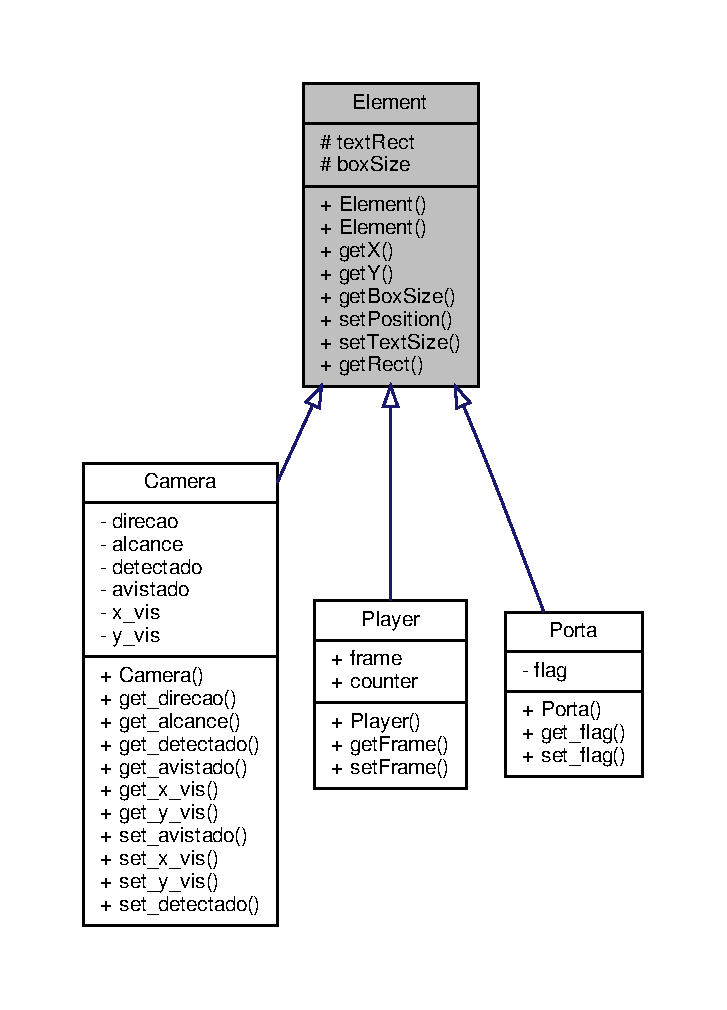
\includegraphics[width=349pt]{classElement__inherit__graph}
\end{center}
\end{figure}


Collaboration diagram for Element\+:
\nopagebreak
\begin{figure}[H]
\begin{center}
\leavevmode
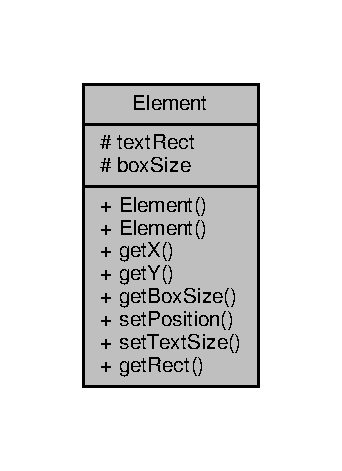
\includegraphics[width=164pt]{classElement__coll__graph}
\end{center}
\end{figure}
\subsection*{Public Member Functions}
\begin{DoxyCompactItemize}
\item 
\hyperlink{classElement_a084081001b0f14ae12d612c866df861c}{Element} ()=default
\begin{DoxyCompactList}\small\item\em Construtor do Elemento default. \end{DoxyCompactList}\item 
\hyperlink{classElement_ae385b104c66f092731777d70775b7f55}{Element} (int x, int y)
\begin{DoxyCompactList}\small\item\em Construtor do Elemento Overloaded\+: define posição. \end{DoxyCompactList}\item 
int \hyperlink{classElement_ab5e2530eac11f0281769e6689856ceb2}{getX} ()
\item 
int \hyperlink{classElement_aad10853bfba140e4ca5cab79d72f2d83}{getY} ()
\item 
int \hyperlink{classElement_a9bb602a1a56055ea4b360b1a5486ff24}{get\+Box\+Size} ()
\item 
void \hyperlink{classElement_a3f07a8ce2682d6bdd56db0ef3de858c0}{set\+Position} (int x, int y)
\item 
void \hyperlink{classElement_af3ad245bd04436524f8bd5c5835bf786}{set\+Text\+Size} (int w, int h)
\item 
S\+D\+L\+\_\+\+Rect $\ast$ \hyperlink{classElement_ac8e7a2a1670e95335b6924b873600ea3}{get\+Rect} ()
\end{DoxyCompactItemize}
\subsection*{Protected Attributes}
\begin{DoxyCompactItemize}
\item 
S\+D\+L\+\_\+\+Rect \hyperlink{classElement_a79d353f4c8bb44fe60390d02571cac64}{text\+Rect}
\item 
int \hyperlink{classElement_a692cd0e79fb7323679a381556a58aaf8}{box\+Size}
\end{DoxyCompactItemize}


\subsection{Detailed Description}
Classe base de Elementos. 

Classe base de Elementos. Outros elementos herdam dessa classe. 

\subsection{Constructor \& Destructor Documentation}
\mbox{\Hypertarget{classElement_a084081001b0f14ae12d612c866df861c}\label{classElement_a084081001b0f14ae12d612c866df861c}} 
\index{Element@{Element}!Element@{Element}}
\index{Element@{Element}!Element@{Element}}
\subsubsection{\texorpdfstring{Element()}{Element()}\hspace{0.1cm}{\footnotesize\ttfamily [1/2]}}
{\footnotesize\ttfamily Element\+::\+Element (\begin{DoxyParamCaption}{ }\end{DoxyParamCaption})\hspace{0.3cm}{\ttfamily [default]}}



Construtor do Elemento default. 

\mbox{\Hypertarget{classElement_ae385b104c66f092731777d70775b7f55}\label{classElement_ae385b104c66f092731777d70775b7f55}} 
\index{Element@{Element}!Element@{Element}}
\index{Element@{Element}!Element@{Element}}
\subsubsection{\texorpdfstring{Element()}{Element()}\hspace{0.1cm}{\footnotesize\ttfamily [2/2]}}
{\footnotesize\ttfamily Element\+::\+Element (\begin{DoxyParamCaption}\item[{int}]{x,  }\item[{int}]{y }\end{DoxyParamCaption})}



Construtor do Elemento Overloaded\+: define posição. 


\begin{DoxyParams}{Parameters}
{\em x} & coordenada x \\
\hline
{\em y} & coordenada y \\
\hline
\end{DoxyParams}


\subsection{Member Function Documentation}
\mbox{\Hypertarget{classElement_a9bb602a1a56055ea4b360b1a5486ff24}\label{classElement_a9bb602a1a56055ea4b360b1a5486ff24}} 
\index{Element@{Element}!get\+Box\+Size@{get\+Box\+Size}}
\index{get\+Box\+Size@{get\+Box\+Size}!Element@{Element}}
\subsubsection{\texorpdfstring{get\+Box\+Size()}{getBoxSize()}}
{\footnotesize\ttfamily int Element\+::get\+Box\+Size (\begin{DoxyParamCaption}{ }\end{DoxyParamCaption})}

\mbox{\Hypertarget{classElement_ac8e7a2a1670e95335b6924b873600ea3}\label{classElement_ac8e7a2a1670e95335b6924b873600ea3}} 
\index{Element@{Element}!get\+Rect@{get\+Rect}}
\index{get\+Rect@{get\+Rect}!Element@{Element}}
\subsubsection{\texorpdfstring{get\+Rect()}{getRect()}}
{\footnotesize\ttfamily S\+D\+L\+\_\+\+Rect $\ast$ Element\+::get\+Rect (\begin{DoxyParamCaption}{ }\end{DoxyParamCaption})}

\mbox{\Hypertarget{classElement_ab5e2530eac11f0281769e6689856ceb2}\label{classElement_ab5e2530eac11f0281769e6689856ceb2}} 
\index{Element@{Element}!getX@{getX}}
\index{getX@{getX}!Element@{Element}}
\subsubsection{\texorpdfstring{get\+X()}{getX()}}
{\footnotesize\ttfamily int Element\+::getX (\begin{DoxyParamCaption}{ }\end{DoxyParamCaption})}

\mbox{\Hypertarget{classElement_aad10853bfba140e4ca5cab79d72f2d83}\label{classElement_aad10853bfba140e4ca5cab79d72f2d83}} 
\index{Element@{Element}!getY@{getY}}
\index{getY@{getY}!Element@{Element}}
\subsubsection{\texorpdfstring{get\+Y()}{getY()}}
{\footnotesize\ttfamily int Element\+::getY (\begin{DoxyParamCaption}{ }\end{DoxyParamCaption})}

\mbox{\Hypertarget{classElement_a3f07a8ce2682d6bdd56db0ef3de858c0}\label{classElement_a3f07a8ce2682d6bdd56db0ef3de858c0}} 
\index{Element@{Element}!set\+Position@{set\+Position}}
\index{set\+Position@{set\+Position}!Element@{Element}}
\subsubsection{\texorpdfstring{set\+Position()}{setPosition()}}
{\footnotesize\ttfamily void Element\+::set\+Position (\begin{DoxyParamCaption}\item[{int}]{x,  }\item[{int}]{y }\end{DoxyParamCaption})}

\mbox{\Hypertarget{classElement_af3ad245bd04436524f8bd5c5835bf786}\label{classElement_af3ad245bd04436524f8bd5c5835bf786}} 
\index{Element@{Element}!set\+Text\+Size@{set\+Text\+Size}}
\index{set\+Text\+Size@{set\+Text\+Size}!Element@{Element}}
\subsubsection{\texorpdfstring{set\+Text\+Size()}{setTextSize()}}
{\footnotesize\ttfamily void Element\+::set\+Text\+Size (\begin{DoxyParamCaption}\item[{int}]{w,  }\item[{int}]{h }\end{DoxyParamCaption})}



\subsection{Member Data Documentation}
\mbox{\Hypertarget{classElement_a692cd0e79fb7323679a381556a58aaf8}\label{classElement_a692cd0e79fb7323679a381556a58aaf8}} 
\index{Element@{Element}!box\+Size@{box\+Size}}
\index{box\+Size@{box\+Size}!Element@{Element}}
\subsubsection{\texorpdfstring{box\+Size}{boxSize}}
{\footnotesize\ttfamily int Element\+::box\+Size\hspace{0.3cm}{\ttfamily [protected]}}

Tamanho do bounding box do Jogador \mbox{\Hypertarget{classElement_a79d353f4c8bb44fe60390d02571cac64}\label{classElement_a79d353f4c8bb44fe60390d02571cac64}} 
\index{Element@{Element}!text\+Rect@{text\+Rect}}
\index{text\+Rect@{text\+Rect}!Element@{Element}}
\subsubsection{\texorpdfstring{text\+Rect}{textRect}}
{\footnotesize\ttfamily S\+D\+L\+\_\+\+Rect Element\+::text\+Rect\hspace{0.3cm}{\ttfamily [protected]}}

Retangulo\+: posicao (x,y) e tamanho (w,h) 

The documentation for this class was generated from the following files\+:\begin{DoxyCompactItemize}
\item 
include/\hyperlink{element_8h}{element.\+h}\item 
src/\hyperlink{element_8cpp}{element.\+cpp}\end{DoxyCompactItemize}

\hypertarget{classEventos}{}\section{Eventos Class Reference}
\label{classEventos}\index{Eventos@{Eventos}}


{\ttfamily \#include $<$eventos.\+h$>$}



Collaboration diagram for Eventos\+:
\nopagebreak
\begin{figure}[H]
\begin{center}
\leavevmode
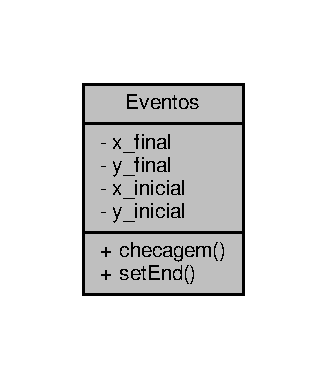
\includegraphics[width=157pt]{classEventos__coll__graph}
\end{center}
\end{figure}
\subsection*{Public Member Functions}
\begin{DoxyCompactItemize}
\item 
int \hyperlink{classEventos_af534be40ac7143eb360a575296ec6b06}{checagem} (\hyperlink{classPlayer}{Player} \&jogador, \hyperlink{classCamera}{Camera} \&camera, int tilesize, int boundingbox)
\begin{DoxyCompactList}\small\item\em Checagem de camera e fim de fase Checar se alguma camera detectou o jogador ou se o jogador chegou no fim da fase. \end{DoxyCompactList}\item 
void \hyperlink{classEventos_a9d2ebdf756c3bb3b0bfe6ad2f73f1202}{set\+End} (int x, int y)
\end{DoxyCompactItemize}
\subsection*{Private Attributes}
\begin{DoxyCompactItemize}
\item 
int \hyperlink{classEventos_afdf3e21f837f2a84c5d258383ada6c29}{x\+\_\+final} = 72$\ast$9
\item 
int \hyperlink{classEventos_a52967e28579a67b2fef4ed6d427a042d}{y\+\_\+final} = 72$\ast$9
\item 
int \hyperlink{classEventos_aa09d32f02896554a3409d0093114cab1}{x\+\_\+inicial} = 0
\item 
int \hyperlink{classEventos_a42c55facc39e42b7c816a06b3009e228}{y\+\_\+inicial} = 0
\end{DoxyCompactItemize}


\subsection{Member Function Documentation}
\mbox{\Hypertarget{classEventos_af534be40ac7143eb360a575296ec6b06}\label{classEventos_af534be40ac7143eb360a575296ec6b06}} 
\index{Eventos@{Eventos}!checagem@{checagem}}
\index{checagem@{checagem}!Eventos@{Eventos}}
\subsubsection{\texorpdfstring{checagem()}{checagem()}}
{\footnotesize\ttfamily int Eventos\+::checagem (\begin{DoxyParamCaption}\item[{\hyperlink{classPlayer}{Player} \&}]{jogador,  }\item[{\hyperlink{classCamera}{Camera} \&}]{camera,  }\item[{int}]{tilesize,  }\item[{int}]{boundingbox }\end{DoxyParamCaption})}



Checagem de camera e fim de fase Checar se alguma camera detectou o jogador ou se o jogador chegou no fim da fase. 


\begin{DoxyParams}{Parameters}
{\em jogador} & Jogador \\
\hline
{\em camera} & \hyperlink{classCamera}{Camera} \\
\hline
{\em tilesize} & Tamanho da textura \\
\hline
{\em boundingbox} & Bounding box do jogador \\
\hline
\end{DoxyParams}
\mbox{\Hypertarget{classEventos_a9d2ebdf756c3bb3b0bfe6ad2f73f1202}\label{classEventos_a9d2ebdf756c3bb3b0bfe6ad2f73f1202}} 
\index{Eventos@{Eventos}!set\+End@{set\+End}}
\index{set\+End@{set\+End}!Eventos@{Eventos}}
\subsubsection{\texorpdfstring{set\+End()}{setEnd()}}
{\footnotesize\ttfamily void Eventos\+::set\+End (\begin{DoxyParamCaption}\item[{int}]{x,  }\item[{int}]{y }\end{DoxyParamCaption})}



\subsection{Member Data Documentation}
\mbox{\Hypertarget{classEventos_afdf3e21f837f2a84c5d258383ada6c29}\label{classEventos_afdf3e21f837f2a84c5d258383ada6c29}} 
\index{Eventos@{Eventos}!x\+\_\+final@{x\+\_\+final}}
\index{x\+\_\+final@{x\+\_\+final}!Eventos@{Eventos}}
\subsubsection{\texorpdfstring{x\+\_\+final}{x\_final}}
{\footnotesize\ttfamily int Eventos\+::x\+\_\+final = 72$\ast$9\hspace{0.3cm}{\ttfamily [private]}}

Coordenada do fim da fase \mbox{\Hypertarget{classEventos_aa09d32f02896554a3409d0093114cab1}\label{classEventos_aa09d32f02896554a3409d0093114cab1}} 
\index{Eventos@{Eventos}!x\+\_\+inicial@{x\+\_\+inicial}}
\index{x\+\_\+inicial@{x\+\_\+inicial}!Eventos@{Eventos}}
\subsubsection{\texorpdfstring{x\+\_\+inicial}{x\_inicial}}
{\footnotesize\ttfamily int Eventos\+::x\+\_\+inicial = 0\hspace{0.3cm}{\ttfamily [private]}}

Coordenada do inicio da fase \mbox{\Hypertarget{classEventos_a52967e28579a67b2fef4ed6d427a042d}\label{classEventos_a52967e28579a67b2fef4ed6d427a042d}} 
\index{Eventos@{Eventos}!y\+\_\+final@{y\+\_\+final}}
\index{y\+\_\+final@{y\+\_\+final}!Eventos@{Eventos}}
\subsubsection{\texorpdfstring{y\+\_\+final}{y\_final}}
{\footnotesize\ttfamily int Eventos\+::y\+\_\+final = 72$\ast$9\hspace{0.3cm}{\ttfamily [private]}}

Coordenada do fim da fase \mbox{\Hypertarget{classEventos_a42c55facc39e42b7c816a06b3009e228}\label{classEventos_a42c55facc39e42b7c816a06b3009e228}} 
\index{Eventos@{Eventos}!y\+\_\+inicial@{y\+\_\+inicial}}
\index{y\+\_\+inicial@{y\+\_\+inicial}!Eventos@{Eventos}}
\subsubsection{\texorpdfstring{y\+\_\+inicial}{y\_inicial}}
{\footnotesize\ttfamily int Eventos\+::y\+\_\+inicial = 0\hspace{0.3cm}{\ttfamily [private]}}

Coordenada do inicio da fase 

The documentation for this class was generated from the following files\+:\begin{DoxyCompactItemize}
\item 
include/\hyperlink{eventos_8h}{eventos.\+h}\item 
src/\hyperlink{eventos_8cpp}{eventos.\+cpp}\end{DoxyCompactItemize}

\hypertarget{classMap}{}\section{Map Class Reference}
\label{classMap}\index{Map@{Map}}


\hyperlink{classMap}{Map} Class.  




{\ttfamily \#include $<$map.\+h$>$}



Collaboration diagram for Map\+:
\nopagebreak
\begin{figure}[H]
\begin{center}
\leavevmode
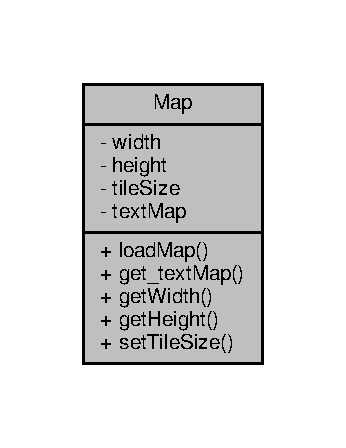
\includegraphics[width=166pt]{classMap__coll__graph}
\end{center}
\end{figure}
\subsection*{Public Member Functions}
\begin{DoxyCompactItemize}
\item 
void \hyperlink{classMap_af48de256cfde701cd70a17bce1c5b727}{load\+Map} (std\+::string map\+File)
\begin{DoxyCompactList}\small\item\em loads the map \end{DoxyCompactList}\item 
std\+::map$<$ std\+::pair$<$ int, int $>$, std\+::string $>$ \& \hyperlink{classMap_ac4b82fa93d76c5891fc18212cd3d9098}{get\+\_\+text\+Map} ()
\item 
int \hyperlink{classMap_afd34d12227676b3cebeed9f5fae2508f}{get\+Width} ()
\item 
int \hyperlink{classMap_a2b09c8875af2efb711fc3a022e70427d}{get\+Height} ()
\item 
void \hyperlink{classMap_a6d9c1f8a1f65316a7a65983ad7ea9ff4}{set\+Tile\+Size} (int size)
\end{DoxyCompactItemize}
\subsection*{Private Attributes}
\begin{DoxyCompactItemize}
\item 
int \hyperlink{classMap_a9ecfe932ad2d2bc22492416033bdacfd}{width}
\item 
int \hyperlink{classMap_a0546fef98caebe38385bb2e0c7a15da1}{height}
\item 
int \hyperlink{classMap_ae686445a21a02aaf586633c5a69e8ff3}{tile\+Size}
\item 
std\+::map$<$ std\+::pair$<$ int, int $>$, std\+::string $>$ \hyperlink{classMap_ae2bfd5c888983cc73be6d9a4c3ad1bcf}{text\+Map}
\end{DoxyCompactItemize}


\subsection{Detailed Description}
\hyperlink{classMap}{Map} Class. 

Mapa é responsável por transformar um arquivo mapa em código em um dicionário (x,y) -\/$>$ textura 

\subsection{Member Function Documentation}
\mbox{\Hypertarget{classMap_ac4b82fa93d76c5891fc18212cd3d9098}\label{classMap_ac4b82fa93d76c5891fc18212cd3d9098}} 
\index{Map@{Map}!get\+\_\+text\+Map@{get\+\_\+text\+Map}}
\index{get\+\_\+text\+Map@{get\+\_\+text\+Map}!Map@{Map}}
\subsubsection{\texorpdfstring{get\+\_\+text\+Map()}{get\_textMap()}}
{\footnotesize\ttfamily std\+::map$<$ std\+::pair$<$ int, int $>$, std\+::string $>$ \& Map\+::get\+\_\+text\+Map (\begin{DoxyParamCaption}{ }\end{DoxyParamCaption})}

Retorna o dicionário por referência \mbox{\Hypertarget{classMap_a2b09c8875af2efb711fc3a022e70427d}\label{classMap_a2b09c8875af2efb711fc3a022e70427d}} 
\index{Map@{Map}!get\+Height@{get\+Height}}
\index{get\+Height@{get\+Height}!Map@{Map}}
\subsubsection{\texorpdfstring{get\+Height()}{getHeight()}}
{\footnotesize\ttfamily int Map\+::get\+Height (\begin{DoxyParamCaption}{ }\end{DoxyParamCaption})}

\mbox{\Hypertarget{classMap_afd34d12227676b3cebeed9f5fae2508f}\label{classMap_afd34d12227676b3cebeed9f5fae2508f}} 
\index{Map@{Map}!get\+Width@{get\+Width}}
\index{get\+Width@{get\+Width}!Map@{Map}}
\subsubsection{\texorpdfstring{get\+Width()}{getWidth()}}
{\footnotesize\ttfamily int Map\+::get\+Width (\begin{DoxyParamCaption}{ }\end{DoxyParamCaption})}

\mbox{\Hypertarget{classMap_af48de256cfde701cd70a17bce1c5b727}\label{classMap_af48de256cfde701cd70a17bce1c5b727}} 
\index{Map@{Map}!load\+Map@{load\+Map}}
\index{load\+Map@{load\+Map}!Map@{Map}}
\subsubsection{\texorpdfstring{load\+Map()}{loadMap()}}
{\footnotesize\ttfamily void Map\+::load\+Map (\begin{DoxyParamCaption}\item[{std\+::string}]{map\+File }\end{DoxyParamCaption})}



loads the map 

Carrega o mapa e o transforma num dicionário 
\begin{DoxyParams}{Parameters}
{\em map\+File} & file (.map) \\
\hline
\end{DoxyParams}
\mbox{\Hypertarget{classMap_a6d9c1f8a1f65316a7a65983ad7ea9ff4}\label{classMap_a6d9c1f8a1f65316a7a65983ad7ea9ff4}} 
\index{Map@{Map}!set\+Tile\+Size@{set\+Tile\+Size}}
\index{set\+Tile\+Size@{set\+Tile\+Size}!Map@{Map}}
\subsubsection{\texorpdfstring{set\+Tile\+Size()}{setTileSize()}}
{\footnotesize\ttfamily void Map\+::set\+Tile\+Size (\begin{DoxyParamCaption}\item[{int}]{size }\end{DoxyParamCaption})}



\subsection{Member Data Documentation}
\mbox{\Hypertarget{classMap_a0546fef98caebe38385bb2e0c7a15da1}\label{classMap_a0546fef98caebe38385bb2e0c7a15da1}} 
\index{Map@{Map}!height@{height}}
\index{height@{height}!Map@{Map}}
\subsubsection{\texorpdfstring{height}{height}}
{\footnotesize\ttfamily int Map\+::height\hspace{0.3cm}{\ttfamily [private]}}

map height \mbox{\Hypertarget{classMap_ae2bfd5c888983cc73be6d9a4c3ad1bcf}\label{classMap_ae2bfd5c888983cc73be6d9a4c3ad1bcf}} 
\index{Map@{Map}!text\+Map@{text\+Map}}
\index{text\+Map@{text\+Map}!Map@{Map}}
\subsubsection{\texorpdfstring{text\+Map}{textMap}}
{\footnotesize\ttfamily std\+::map$<$std\+::pair$<$int, int$>$, std\+::string$>$ Map\+::text\+Map\hspace{0.3cm}{\ttfamily [private]}}

Mapa (x,y)-\/$>$ texture\+File \mbox{\Hypertarget{classMap_ae686445a21a02aaf586633c5a69e8ff3}\label{classMap_ae686445a21a02aaf586633c5a69e8ff3}} 
\index{Map@{Map}!tile\+Size@{tile\+Size}}
\index{tile\+Size@{tile\+Size}!Map@{Map}}
\subsubsection{\texorpdfstring{tile\+Size}{tileSize}}
{\footnotesize\ttfamily int Map\+::tile\+Size\hspace{0.3cm}{\ttfamily [private]}}

size of 1 side of tile (always a square) \mbox{\Hypertarget{classMap_a9ecfe932ad2d2bc22492416033bdacfd}\label{classMap_a9ecfe932ad2d2bc22492416033bdacfd}} 
\index{Map@{Map}!width@{width}}
\index{width@{width}!Map@{Map}}
\subsubsection{\texorpdfstring{width}{width}}
{\footnotesize\ttfamily int Map\+::width\hspace{0.3cm}{\ttfamily [private]}}

map width 

The documentation for this class was generated from the following files\+:\begin{DoxyCompactItemize}
\item 
include/\hyperlink{map_8h}{map.\+h}\item 
src/\hyperlink{map_8cpp}{map.\+cpp}\end{DoxyCompactItemize}

\hypertarget{classPlayer}{}\section{Player Class Reference}
\label{classPlayer}\index{Player@{Player}}


Classe \hyperlink{classPlayer}{Player}.  




{\ttfamily \#include $<$player.\+h$>$}



Inheritance diagram for Player\+:
\nopagebreak
\begin{figure}[H]
\begin{center}
\leavevmode
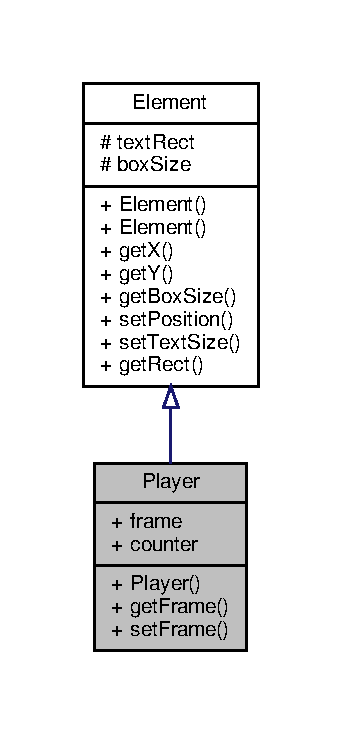
\includegraphics[width=164pt]{classPlayer__inherit__graph}
\end{center}
\end{figure}


Collaboration diagram for Player\+:
\nopagebreak
\begin{figure}[H]
\begin{center}
\leavevmode
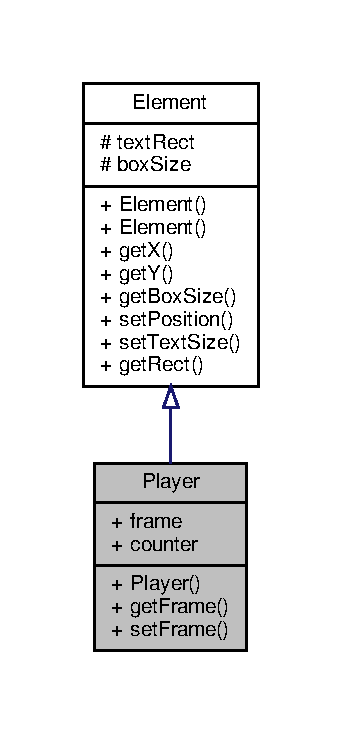
\includegraphics[width=164pt]{classPlayer__coll__graph}
\end{center}
\end{figure}
\subsection*{Public Member Functions}
\begin{DoxyCompactItemize}
\item 
\hyperlink{classPlayer_a9b009cc0bebdcc27a837d50b1f4ededd}{Player} (int x, int y)
\begin{DoxyCompactList}\small\item\em Construtor do \hyperlink{classPlayer}{Player} Define posição. \end{DoxyCompactList}\item 
int \hyperlink{classPlayer_a73374c899105e2ba7fab9340d279e3a0}{get\+Frame} ()
\item 
void \hyperlink{classPlayer_a0b5112993f246d3c0a848f3eab8db3a8}{set\+Frame} (std\+::string s)
\end{DoxyCompactItemize}
\subsection*{Public Attributes}
\begin{DoxyCompactItemize}
\item 
int \hyperlink{classPlayer_a4af20962be9096bdc5571ee9f9bf3a29}{frame} = 0
\item 
int \hyperlink{classPlayer_a03eea1e12f10153b96d2c79f906fcc14}{counter} = 0
\end{DoxyCompactItemize}
\subsection*{Additional Inherited Members}


\subsection{Detailed Description}
Classe \hyperlink{classPlayer}{Player}. 

Herda de Elementos. Adiciona controle de frames (animação) 

\subsection{Constructor \& Destructor Documentation}
\mbox{\Hypertarget{classPlayer_a9b009cc0bebdcc27a837d50b1f4ededd}\label{classPlayer_a9b009cc0bebdcc27a837d50b1f4ededd}} 
\index{Player@{Player}!Player@{Player}}
\index{Player@{Player}!Player@{Player}}
\subsubsection{\texorpdfstring{Player()}{Player()}}
{\footnotesize\ttfamily Player\+::\+Player (\begin{DoxyParamCaption}\item[{int}]{x,  }\item[{int}]{y }\end{DoxyParamCaption})}



Construtor do \hyperlink{classPlayer}{Player} Define posição. 


\begin{DoxyParams}{Parameters}
{\em x} & coordenada x \\
\hline
{\em y} & coordenada y \\
\hline
\end{DoxyParams}


\subsection{Member Function Documentation}
\mbox{\Hypertarget{classPlayer_a73374c899105e2ba7fab9340d279e3a0}\label{classPlayer_a73374c899105e2ba7fab9340d279e3a0}} 
\index{Player@{Player}!get\+Frame@{get\+Frame}}
\index{get\+Frame@{get\+Frame}!Player@{Player}}
\subsubsection{\texorpdfstring{get\+Frame()}{getFrame()}}
{\footnotesize\ttfamily int Player\+::get\+Frame (\begin{DoxyParamCaption}{ }\end{DoxyParamCaption})}

\mbox{\Hypertarget{classPlayer_a0b5112993f246d3c0a848f3eab8db3a8}\label{classPlayer_a0b5112993f246d3c0a848f3eab8db3a8}} 
\index{Player@{Player}!set\+Frame@{set\+Frame}}
\index{set\+Frame@{set\+Frame}!Player@{Player}}
\subsubsection{\texorpdfstring{set\+Frame()}{setFrame()}}
{\footnotesize\ttfamily void Player\+::set\+Frame (\begin{DoxyParamCaption}\item[{std\+::string}]{s }\end{DoxyParamCaption})}



\subsection{Member Data Documentation}
\mbox{\Hypertarget{classPlayer_a03eea1e12f10153b96d2c79f906fcc14}\label{classPlayer_a03eea1e12f10153b96d2c79f906fcc14}} 
\index{Player@{Player}!counter@{counter}}
\index{counter@{counter}!Player@{Player}}
\subsubsection{\texorpdfstring{counter}{counter}}
{\footnotesize\ttfamily int Player\+::counter = 0}

Contador para controle \mbox{\Hypertarget{classPlayer_a4af20962be9096bdc5571ee9f9bf3a29}\label{classPlayer_a4af20962be9096bdc5571ee9f9bf3a29}} 
\index{Player@{Player}!frame@{frame}}
\index{frame@{frame}!Player@{Player}}
\subsubsection{\texorpdfstring{frame}{frame}}
{\footnotesize\ttfamily int Player\+::frame = 0}

Frame atual 

The documentation for this class was generated from the following files\+:\begin{DoxyCompactItemize}
\item 
include/\hyperlink{player_8h}{player.\+h}\item 
src/\hyperlink{player_8cpp}{player.\+cpp}\end{DoxyCompactItemize}

\hypertarget{classPorta}{}\section{Porta Class Reference}
\label{classPorta}\index{Porta@{Porta}}


{\ttfamily \#include $<$porta.\+h$>$}



Inheritance diagram for Porta\+:
\nopagebreak
\begin{figure}[H]
\begin{center}
\leavevmode
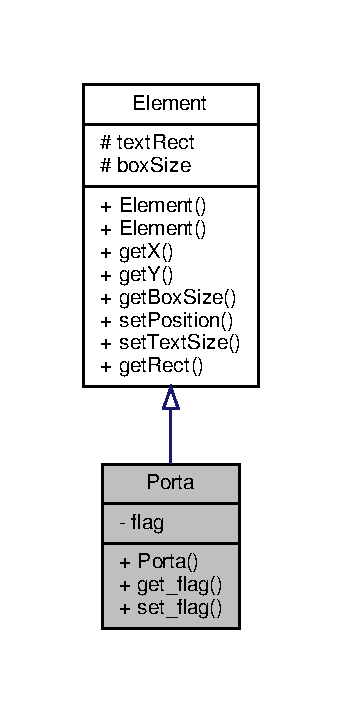
\includegraphics[width=164pt]{classPorta__inherit__graph}
\end{center}
\end{figure}


Collaboration diagram for Porta\+:
\nopagebreak
\begin{figure}[H]
\begin{center}
\leavevmode
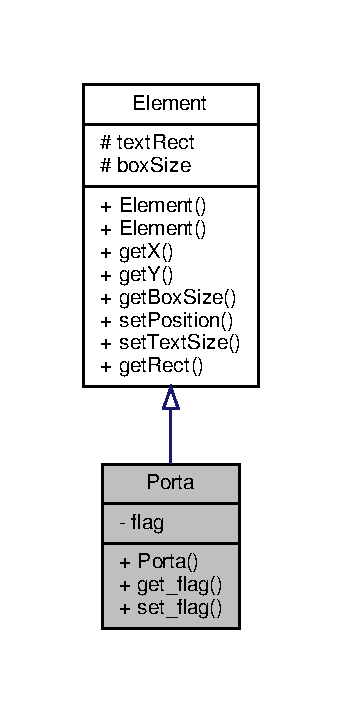
\includegraphics[width=164pt]{classPorta__coll__graph}
\end{center}
\end{figure}
\subsection*{Public Member Functions}
\begin{DoxyCompactItemize}
\item 
\hyperlink{classPorta_aa17fba5ecd6f7c8a59ec75a15526d6cc}{Porta} (int x, int y, int \hyperlink{classPorta_a8db544173490043789a14eaae3bf8ed6}{flag})
\item 
int \hyperlink{classPorta_ae2c04fc5bf8ddce2195252c526f653b8}{get\+\_\+flag} ()
\item 
void \hyperlink{classPorta_a3ac51e6aa3d03be6bf01a73e748cf435}{set\+\_\+flag} (int \hyperlink{classPorta_a8db544173490043789a14eaae3bf8ed6}{flag})
\end{DoxyCompactItemize}
\subsection*{Private Attributes}
\begin{DoxyCompactItemize}
\item 
int \hyperlink{classPorta_a8db544173490043789a14eaae3bf8ed6}{flag}
\end{DoxyCompactItemize}
\subsection*{Additional Inherited Members}


\subsection{Constructor \& Destructor Documentation}
\mbox{\Hypertarget{classPorta_aa17fba5ecd6f7c8a59ec75a15526d6cc}\label{classPorta_aa17fba5ecd6f7c8a59ec75a15526d6cc}} 
\index{Porta@{Porta}!Porta@{Porta}}
\index{Porta@{Porta}!Porta@{Porta}}
\subsubsection{\texorpdfstring{Porta()}{Porta()}}
{\footnotesize\ttfamily Porta\+::\+Porta (\begin{DoxyParamCaption}\item[{int}]{x,  }\item[{int}]{y,  }\item[{int}]{flag }\end{DoxyParamCaption})}



\subsection{Member Function Documentation}
\mbox{\Hypertarget{classPorta_ae2c04fc5bf8ddce2195252c526f653b8}\label{classPorta_ae2c04fc5bf8ddce2195252c526f653b8}} 
\index{Porta@{Porta}!get\+\_\+flag@{get\+\_\+flag}}
\index{get\+\_\+flag@{get\+\_\+flag}!Porta@{Porta}}
\subsubsection{\texorpdfstring{get\+\_\+flag()}{get\_flag()}}
{\footnotesize\ttfamily int Porta\+::get\+\_\+flag (\begin{DoxyParamCaption}{ }\end{DoxyParamCaption})}

\mbox{\Hypertarget{classPorta_a3ac51e6aa3d03be6bf01a73e748cf435}\label{classPorta_a3ac51e6aa3d03be6bf01a73e748cf435}} 
\index{Porta@{Porta}!set\+\_\+flag@{set\+\_\+flag}}
\index{set\+\_\+flag@{set\+\_\+flag}!Porta@{Porta}}
\subsubsection{\texorpdfstring{set\+\_\+flag()}{set\_flag()}}
{\footnotesize\ttfamily void Porta\+::set\+\_\+flag (\begin{DoxyParamCaption}\item[{int}]{flag }\end{DoxyParamCaption})}



\subsection{Member Data Documentation}
\mbox{\Hypertarget{classPorta_a8db544173490043789a14eaae3bf8ed6}\label{classPorta_a8db544173490043789a14eaae3bf8ed6}} 
\index{Porta@{Porta}!flag@{flag}}
\index{flag@{flag}!Porta@{Porta}}
\subsubsection{\texorpdfstring{flag}{flag}}
{\footnotesize\ttfamily int Porta\+::flag\hspace{0.3cm}{\ttfamily [private]}}



The documentation for this class was generated from the following files\+:\begin{DoxyCompactItemize}
\item 
include/\hyperlink{porta_8h}{porta.\+h}\item 
src/\hyperlink{porta_8cpp}{porta.\+cpp}\end{DoxyCompactItemize}

\hypertarget{classPorta__controller}{}\section{Porta\+\_\+controller Class Reference}
\label{classPorta__controller}\index{Porta\+\_\+controller@{Porta\+\_\+controller}}


{\ttfamily \#include $<$porta\+\_\+controller.\+h$>$}



Collaboration diagram for Porta\+\_\+controller\+:
\nopagebreak
\begin{figure}[H]
\begin{center}
\leavevmode
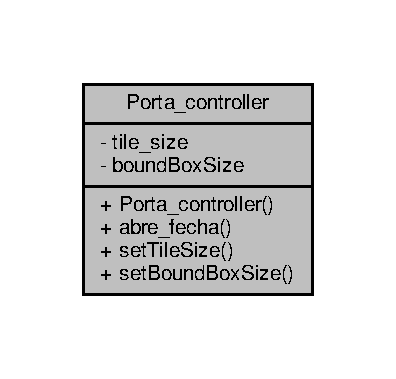
\includegraphics[width=190pt]{classPorta__controller__coll__graph}
\end{center}
\end{figure}
\subsection*{Public Member Functions}
\begin{DoxyCompactItemize}
\item 
\hyperlink{classPorta__controller_a89cf75aa5f2ce1658a8bb79ddd5d2f7a}{Porta\+\_\+controller} ()=default
\item 
void \hyperlink{classPorta__controller_a48b56002e2e7c95fccab3b46f4724c40}{abre\+\_\+fecha} (\hyperlink{classPorta}{Porta} \&porta, \hyperlink{classPlayer}{Player} \&jogador, \hyperlink{classMap}{Map} \&mapa, const Uint8 $\ast$state, int $\ast$$\ast$collision\+Map)
\item 
void \hyperlink{classPorta__controller_a372c8535da4c433e4d512a62c8169b57}{set\+Tile\+Size} (int s)
\item 
void \hyperlink{classPorta__controller_adbfa18c658caec1bd169e95a36de0d20}{set\+Bound\+Box\+Size} (int s)
\end{DoxyCompactItemize}
\subsection*{Private Attributes}
\begin{DoxyCompactItemize}
\item 
int \hyperlink{classPorta__controller_a5dd2267f5f11f53019a5418d1d4e9538}{tile\+\_\+size} = 0
\item 
int \hyperlink{classPorta__controller_a756d8d4a02fe24564c0c184f447f0933}{bound\+Box\+Size} = 0
\end{DoxyCompactItemize}


\subsection{Constructor \& Destructor Documentation}
\mbox{\Hypertarget{classPorta__controller_a89cf75aa5f2ce1658a8bb79ddd5d2f7a}\label{classPorta__controller_a89cf75aa5f2ce1658a8bb79ddd5d2f7a}} 
\index{Porta\+\_\+controller@{Porta\+\_\+controller}!Porta\+\_\+controller@{Porta\+\_\+controller}}
\index{Porta\+\_\+controller@{Porta\+\_\+controller}!Porta\+\_\+controller@{Porta\+\_\+controller}}
\subsubsection{\texorpdfstring{Porta\+\_\+controller()}{Porta\_controller()}}
{\footnotesize\ttfamily Porta\+\_\+controller\+::\+Porta\+\_\+controller (\begin{DoxyParamCaption}{ }\end{DoxyParamCaption})\hspace{0.3cm}{\ttfamily [default]}}



\subsection{Member Function Documentation}
\mbox{\Hypertarget{classPorta__controller_a48b56002e2e7c95fccab3b46f4724c40}\label{classPorta__controller_a48b56002e2e7c95fccab3b46f4724c40}} 
\index{Porta\+\_\+controller@{Porta\+\_\+controller}!abre\+\_\+fecha@{abre\+\_\+fecha}}
\index{abre\+\_\+fecha@{abre\+\_\+fecha}!Porta\+\_\+controller@{Porta\+\_\+controller}}
\subsubsection{\texorpdfstring{abre\+\_\+fecha()}{abre\_fecha()}}
{\footnotesize\ttfamily void Porta\+\_\+controller\+::abre\+\_\+fecha (\begin{DoxyParamCaption}\item[{\hyperlink{classPorta}{Porta} \&}]{porta,  }\item[{\hyperlink{classPlayer}{Player} \&}]{jogador,  }\item[{\hyperlink{classMap}{Map} \&}]{mapa,  }\item[{const Uint8 $\ast$}]{state,  }\item[{int $\ast$$\ast$}]{collision\+Map }\end{DoxyParamCaption})}

\mbox{\Hypertarget{classPorta__controller_adbfa18c658caec1bd169e95a36de0d20}\label{classPorta__controller_adbfa18c658caec1bd169e95a36de0d20}} 
\index{Porta\+\_\+controller@{Porta\+\_\+controller}!set\+Bound\+Box\+Size@{set\+Bound\+Box\+Size}}
\index{set\+Bound\+Box\+Size@{set\+Bound\+Box\+Size}!Porta\+\_\+controller@{Porta\+\_\+controller}}
\subsubsection{\texorpdfstring{set\+Bound\+Box\+Size()}{setBoundBoxSize()}}
{\footnotesize\ttfamily void Porta\+\_\+controller\+::set\+Bound\+Box\+Size (\begin{DoxyParamCaption}\item[{int}]{s }\end{DoxyParamCaption})}

\mbox{\Hypertarget{classPorta__controller_a372c8535da4c433e4d512a62c8169b57}\label{classPorta__controller_a372c8535da4c433e4d512a62c8169b57}} 
\index{Porta\+\_\+controller@{Porta\+\_\+controller}!set\+Tile\+Size@{set\+Tile\+Size}}
\index{set\+Tile\+Size@{set\+Tile\+Size}!Porta\+\_\+controller@{Porta\+\_\+controller}}
\subsubsection{\texorpdfstring{set\+Tile\+Size()}{setTileSize()}}
{\footnotesize\ttfamily void Porta\+\_\+controller\+::set\+Tile\+Size (\begin{DoxyParamCaption}\item[{int}]{s }\end{DoxyParamCaption})}



\subsection{Member Data Documentation}
\mbox{\Hypertarget{classPorta__controller_a756d8d4a02fe24564c0c184f447f0933}\label{classPorta__controller_a756d8d4a02fe24564c0c184f447f0933}} 
\index{Porta\+\_\+controller@{Porta\+\_\+controller}!bound\+Box\+Size@{bound\+Box\+Size}}
\index{bound\+Box\+Size@{bound\+Box\+Size}!Porta\+\_\+controller@{Porta\+\_\+controller}}
\subsubsection{\texorpdfstring{bound\+Box\+Size}{boundBoxSize}}
{\footnotesize\ttfamily int Porta\+\_\+controller\+::bound\+Box\+Size = 0\hspace{0.3cm}{\ttfamily [private]}}

\mbox{\Hypertarget{classPorta__controller_a5dd2267f5f11f53019a5418d1d4e9538}\label{classPorta__controller_a5dd2267f5f11f53019a5418d1d4e9538}} 
\index{Porta\+\_\+controller@{Porta\+\_\+controller}!tile\+\_\+size@{tile\+\_\+size}}
\index{tile\+\_\+size@{tile\+\_\+size}!Porta\+\_\+controller@{Porta\+\_\+controller}}
\subsubsection{\texorpdfstring{tile\+\_\+size}{tile\_size}}
{\footnotesize\ttfamily int Porta\+\_\+controller\+::tile\+\_\+size = 0\hspace{0.3cm}{\ttfamily [private]}}



The documentation for this class was generated from the following files\+:\begin{DoxyCompactItemize}
\item 
include/\hyperlink{porta__controller_8h}{porta\+\_\+controller.\+h}\item 
src/\hyperlink{porta__controller_8cpp}{porta\+\_\+controller.\+cpp}\end{DoxyCompactItemize}

\hypertarget{classViewer}{}\section{Viewer Class Reference}
\label{classViewer}\index{Viewer@{Viewer}}


{\ttfamily \#include $<$viewer.\+h$>$}



Collaboration diagram for Viewer\+:
\nopagebreak
\begin{figure}[H]
\begin{center}
\leavevmode
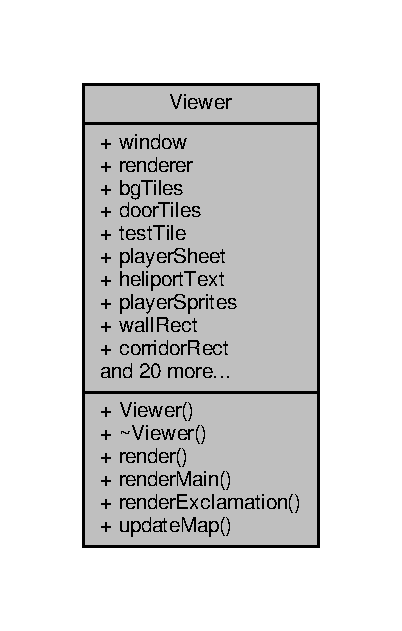
\includegraphics[width=193pt]{classViewer__coll__graph}
\end{center}
\end{figure}
\subsection*{Public Member Functions}
\begin{DoxyCompactItemize}
\item 
\hyperlink{classViewer_aaedebacb31cba87de6e7d448ed8d6586}{Viewer} ()
\begin{DoxyCompactList}\small\item\em Construtor do \hyperlink{classViewer}{Viewer} Configura e inicializa o renderizador. Monta o dicionário de texturas. \end{DoxyCompactList}\item 
\hyperlink{classViewer_a324e5a6a1532fe5eac3f3b0e4792b2da}{$\sim$\+Viewer} ()
\begin{DoxyCompactList}\small\item\em Destrutor do \hyperlink{classViewer}{Viewer} Destroi texturas e o Renderizador. \end{DoxyCompactList}\item 
void \hyperlink{classViewer_a335d914ec8088b5917df9ec465f7a7aa}{render} (\hyperlink{classPlayer}{Player} \&player)
\item 
void \hyperlink{classViewer_a2f6616a8c04e79b4251c7d1aaf1d3aaa}{render\+Main} ()
\item 
void \hyperlink{classViewer_abf19deab378a650856e92ab4f4e42126}{render\+Exclamation} (\hyperlink{classCamera}{Camera} \&cam)
\item 
void \hyperlink{classViewer_ab9787f02682d9e2b699ab16cd20fe43a}{update\+Map} (std\+::map$<$ std\+::pair$<$ int, int $>$, std\+::string $>$ \&\hyperlink{classViewer_a34e0e3043d5155be7fbaef0b07b647f8}{text\+Map})
\end{DoxyCompactItemize}
\subsection*{Public Attributes}
\begin{DoxyCompactItemize}
\item 
S\+D\+L\+\_\+\+Window $\ast$ \hyperlink{classViewer_a9f4bbe40df531d56d30098af395bfd42}{window}
\item 
S\+D\+L\+\_\+\+Renderer $\ast$ \hyperlink{classViewer_aa242869e70efed8cbd51e0345db286d5}{renderer}
\item 
S\+D\+L\+\_\+\+Texture $\ast$ \hyperlink{classViewer_a05710c1f079a9099419fd1882643a349}{bg\+Tiles}
\item 
S\+D\+L\+\_\+\+Texture $\ast$ \hyperlink{classViewer_a9c91a1e8d706ae06579922ba31088775}{door\+Tiles}
\item 
S\+D\+L\+\_\+\+Texture $\ast$ \hyperlink{classViewer_a68100cc46ca81331b8eb394de47ead87}{test\+Tile}
\item 
S\+D\+L\+\_\+\+Texture $\ast$ \hyperlink{classViewer_a9bb70fa5cb5dd60d328cee1f6b23c7de}{player\+Sheet}
\item 
S\+D\+L\+\_\+\+Texture $\ast$ \hyperlink{classViewer_a6885109c94a29d43259967707ab3910e}{heliport\+Text}
\item 
std\+::vector$<$ S\+D\+L\+\_\+\+Rect $\ast$ $>$ \hyperlink{classViewer_a29c1477b7847d678e5927ccfa5950969}{player\+Sprites}
\item 
S\+D\+L\+\_\+\+Rect \hyperlink{classViewer_a5475b38369314f06da131e7ca558dec0}{wall\+Rect}
\item 
S\+D\+L\+\_\+\+Rect \hyperlink{classViewer_abc5bc66b70995658bc7485a83a66555d}{corridor\+Rect}
\item 
S\+D\+L\+\_\+\+Rect \hyperlink{classViewer_a43249e2007827e3cd55529efd37c528d}{porta\+Fechada\+Rect}
\item 
S\+D\+L\+\_\+\+Rect \hyperlink{classViewer_a6c875f769828a91e54df3c5c379e74a1}{porta\+Aberta\+Rect}
\item 
S\+D\+L\+\_\+\+Rect \hyperlink{classViewer_a2564f386e8d491f4a3a52cd21037b0ab}{camera\+Cima\+Rect}
\item 
S\+D\+L\+\_\+\+Rect \hyperlink{classViewer_a8cd66938fa5418497e5f8bb877960409}{camera\+Cima\+Dir\+Rect}
\item 
S\+D\+L\+\_\+\+Rect \hyperlink{classViewer_af8303b86bd4da1c5d93042b9c9a091f5}{camera\+Cima\+Esq\+Rect}
\item 
S\+D\+L\+\_\+\+Rect \hyperlink{classViewer_a95a1339fd00bd739da9e6c2bd05e95ec}{camera\+Baixo\+Rect}
\item 
S\+D\+L\+\_\+\+Rect \hyperlink{classViewer_aaad98d13a259888e00ed2d58ca4645a2}{camera\+Baixo\+Dir\+Rect}
\item 
S\+D\+L\+\_\+\+Rect \hyperlink{classViewer_a036f0479074b0bf9c1e74ce55d262a6b}{camera\+Baixo\+Esq\+Rect}
\item 
S\+D\+L\+\_\+\+Rect \hyperlink{classViewer_a03275a5d07e4096525ec9e3168268dd6}{camera\+Esq\+Rect}
\item 
S\+D\+L\+\_\+\+Rect \hyperlink{classViewer_a802293c85d676e0ceca2637312e9ca61}{camera\+Dir\+Rect}
\item 
std\+::map$<$ std\+::string, std\+::pair$<$ S\+D\+L\+\_\+\+Texture $\ast$, S\+D\+L\+\_\+\+Rect $\ast$ $>$ $>$ \hyperlink{classViewer_a336123429ce452088ba9833f8f80cfff}{text\+Dict}
\item 
S\+D\+L\+\_\+\+Texture $\ast$ \hyperlink{classViewer_a1bad0e9a1333a329d968d289938265a5}{main\+Title}
\item 
S\+D\+L\+\_\+\+Texture $\ast$ \hyperlink{classViewer_a9b3c83a12e44f5761001b4dd5369cf4f}{exclamation\+Text}
\item 
std\+::map$<$ std\+::pair$<$ int, int $>$, std\+::string $>$ \hyperlink{classViewer_a34e0e3043d5155be7fbaef0b07b647f8}{text\+Map}
\item 
S\+D\+L\+\_\+\+Rect \hyperlink{classViewer_a7e38c4e4399e4e4f4d9a1a148843d7f5}{tile\+Rect}
\item 
S\+D\+L\+\_\+\+Event \hyperlink{classViewer_a15a2d333c70e4d16bd85368bdbffaec7}{evento}
\item 
int \hyperlink{classViewer_a1c2c61744bd1f39a6c99671105eee03d}{tile\+Size} = 72
\item 
const int \hyperlink{classViewer_a57814822429ca824ac0c3d355df4ec78}{S\+C\+R\+E\+E\+N\+\_\+\+W\+I\+D\+TH} = 10$\ast$\hyperlink{classViewer_a1c2c61744bd1f39a6c99671105eee03d}{tile\+Size}
\item 
const int \hyperlink{classViewer_a20f47b2f2d1558fff5feb4dfe075f9fc}{S\+C\+R\+E\+E\+N\+\_\+\+H\+E\+I\+G\+HT} = 10$\ast$\hyperlink{classViewer_a1c2c61744bd1f39a6c99671105eee03d}{tile\+Size}
\item 
const Uint8 $\ast$ \hyperlink{classViewer_a2c820741a53119711fa1f43b812aa33b}{state} = S\+D\+L\+\_\+\+Get\+Keyboard\+State(nullptr)
\end{DoxyCompactItemize}


\subsection{Constructor \& Destructor Documentation}
\mbox{\Hypertarget{classViewer_aaedebacb31cba87de6e7d448ed8d6586}\label{classViewer_aaedebacb31cba87de6e7d448ed8d6586}} 
\index{Viewer@{Viewer}!Viewer@{Viewer}}
\index{Viewer@{Viewer}!Viewer@{Viewer}}
\subsubsection{\texorpdfstring{Viewer()}{Viewer()}}
{\footnotesize\ttfamily Viewer\+::\+Viewer (\begin{DoxyParamCaption}{ }\end{DoxyParamCaption})}



Construtor do \hyperlink{classViewer}{Viewer} Configura e inicializa o renderizador. Monta o dicionário de texturas. 

\mbox{\Hypertarget{classViewer_a324e5a6a1532fe5eac3f3b0e4792b2da}\label{classViewer_a324e5a6a1532fe5eac3f3b0e4792b2da}} 
\index{Viewer@{Viewer}!````~Viewer@{$\sim$\+Viewer}}
\index{````~Viewer@{$\sim$\+Viewer}!Viewer@{Viewer}}
\subsubsection{\texorpdfstring{$\sim$\+Viewer()}{~Viewer()}}
{\footnotesize\ttfamily Viewer\+::$\sim$\+Viewer (\begin{DoxyParamCaption}{ }\end{DoxyParamCaption})}



Destrutor do \hyperlink{classViewer}{Viewer} Destroi texturas e o Renderizador. 



\subsection{Member Function Documentation}
\mbox{\Hypertarget{classViewer_a335d914ec8088b5917df9ec465f7a7aa}\label{classViewer_a335d914ec8088b5917df9ec465f7a7aa}} 
\index{Viewer@{Viewer}!render@{render}}
\index{render@{render}!Viewer@{Viewer}}
\subsubsection{\texorpdfstring{render()}{render()}}
{\footnotesize\ttfamily void Viewer\+::render (\begin{DoxyParamCaption}\item[{\hyperlink{classPlayer}{Player} \&}]{player }\end{DoxyParamCaption})}

Renderiza a cena 
\begin{DoxyParams}{Parameters}
{\em player} & Jogador a ser renderizado \\
\hline
\end{DoxyParams}
\mbox{\Hypertarget{classViewer_abf19deab378a650856e92ab4f4e42126}\label{classViewer_abf19deab378a650856e92ab4f4e42126}} 
\index{Viewer@{Viewer}!render\+Exclamation@{render\+Exclamation}}
\index{render\+Exclamation@{render\+Exclamation}!Viewer@{Viewer}}
\subsubsection{\texorpdfstring{render\+Exclamation()}{renderExclamation()}}
{\footnotesize\ttfamily void Viewer\+::render\+Exclamation (\begin{DoxyParamCaption}\item[{\hyperlink{classCamera}{Camera} \&}]{cam }\end{DoxyParamCaption})}

Renderiza o sinal de deteccao \mbox{\Hypertarget{classViewer_a2f6616a8c04e79b4251c7d1aaf1d3aaa}\label{classViewer_a2f6616a8c04e79b4251c7d1aaf1d3aaa}} 
\index{Viewer@{Viewer}!render\+Main@{render\+Main}}
\index{render\+Main@{render\+Main}!Viewer@{Viewer}}
\subsubsection{\texorpdfstring{render\+Main()}{renderMain()}}
{\footnotesize\ttfamily void Viewer\+::render\+Main (\begin{DoxyParamCaption}{ }\end{DoxyParamCaption})}

Renderiza a tela principal \mbox{\Hypertarget{classViewer_ab9787f02682d9e2b699ab16cd20fe43a}\label{classViewer_ab9787f02682d9e2b699ab16cd20fe43a}} 
\index{Viewer@{Viewer}!update\+Map@{update\+Map}}
\index{update\+Map@{update\+Map}!Viewer@{Viewer}}
\subsubsection{\texorpdfstring{update\+Map()}{updateMap()}}
{\footnotesize\ttfamily void Viewer\+::update\+Map (\begin{DoxyParamCaption}\item[{std\+::map$<$ std\+::pair$<$ int, int $>$, std\+::string $>$ \&}]{text\+Map }\end{DoxyParamCaption})}

Guarda uma referencia para o dicionario do mapa 

\subsection{Member Data Documentation}
\mbox{\Hypertarget{classViewer_a05710c1f079a9099419fd1882643a349}\label{classViewer_a05710c1f079a9099419fd1882643a349}} 
\index{Viewer@{Viewer}!bg\+Tiles@{bg\+Tiles}}
\index{bg\+Tiles@{bg\+Tiles}!Viewer@{Viewer}}
\subsubsection{\texorpdfstring{bg\+Tiles}{bgTiles}}
{\footnotesize\ttfamily S\+D\+L\+\_\+\+Texture$\ast$ Viewer\+::bg\+Tiles}

Tile\+Sheet \mbox{\Hypertarget{classViewer_aaad98d13a259888e00ed2d58ca4645a2}\label{classViewer_aaad98d13a259888e00ed2d58ca4645a2}} 
\index{Viewer@{Viewer}!camera\+Baixo\+Dir\+Rect@{camera\+Baixo\+Dir\+Rect}}
\index{camera\+Baixo\+Dir\+Rect@{camera\+Baixo\+Dir\+Rect}!Viewer@{Viewer}}
\subsubsection{\texorpdfstring{camera\+Baixo\+Dir\+Rect}{cameraBaixoDirRect}}
{\footnotesize\ttfamily S\+D\+L\+\_\+\+Rect Viewer\+::camera\+Baixo\+Dir\+Rect}

Tile Source Rectangles \mbox{\Hypertarget{classViewer_a036f0479074b0bf9c1e74ce55d262a6b}\label{classViewer_a036f0479074b0bf9c1e74ce55d262a6b}} 
\index{Viewer@{Viewer}!camera\+Baixo\+Esq\+Rect@{camera\+Baixo\+Esq\+Rect}}
\index{camera\+Baixo\+Esq\+Rect@{camera\+Baixo\+Esq\+Rect}!Viewer@{Viewer}}
\subsubsection{\texorpdfstring{camera\+Baixo\+Esq\+Rect}{cameraBaixoEsqRect}}
{\footnotesize\ttfamily S\+D\+L\+\_\+\+Rect Viewer\+::camera\+Baixo\+Esq\+Rect}

Tile Source Rectangles \mbox{\Hypertarget{classViewer_a95a1339fd00bd739da9e6c2bd05e95ec}\label{classViewer_a95a1339fd00bd739da9e6c2bd05e95ec}} 
\index{Viewer@{Viewer}!camera\+Baixo\+Rect@{camera\+Baixo\+Rect}}
\index{camera\+Baixo\+Rect@{camera\+Baixo\+Rect}!Viewer@{Viewer}}
\subsubsection{\texorpdfstring{camera\+Baixo\+Rect}{cameraBaixoRect}}
{\footnotesize\ttfamily S\+D\+L\+\_\+\+Rect Viewer\+::camera\+Baixo\+Rect}

Tile Source Rectangles \mbox{\Hypertarget{classViewer_a8cd66938fa5418497e5f8bb877960409}\label{classViewer_a8cd66938fa5418497e5f8bb877960409}} 
\index{Viewer@{Viewer}!camera\+Cima\+Dir\+Rect@{camera\+Cima\+Dir\+Rect}}
\index{camera\+Cima\+Dir\+Rect@{camera\+Cima\+Dir\+Rect}!Viewer@{Viewer}}
\subsubsection{\texorpdfstring{camera\+Cima\+Dir\+Rect}{cameraCimaDirRect}}
{\footnotesize\ttfamily S\+D\+L\+\_\+\+Rect Viewer\+::camera\+Cima\+Dir\+Rect}

Tile Source Rectangles \mbox{\Hypertarget{classViewer_af8303b86bd4da1c5d93042b9c9a091f5}\label{classViewer_af8303b86bd4da1c5d93042b9c9a091f5}} 
\index{Viewer@{Viewer}!camera\+Cima\+Esq\+Rect@{camera\+Cima\+Esq\+Rect}}
\index{camera\+Cima\+Esq\+Rect@{camera\+Cima\+Esq\+Rect}!Viewer@{Viewer}}
\subsubsection{\texorpdfstring{camera\+Cima\+Esq\+Rect}{cameraCimaEsqRect}}
{\footnotesize\ttfamily S\+D\+L\+\_\+\+Rect Viewer\+::camera\+Cima\+Esq\+Rect}

Tile Source Rectangles \mbox{\Hypertarget{classViewer_a2564f386e8d491f4a3a52cd21037b0ab}\label{classViewer_a2564f386e8d491f4a3a52cd21037b0ab}} 
\index{Viewer@{Viewer}!camera\+Cima\+Rect@{camera\+Cima\+Rect}}
\index{camera\+Cima\+Rect@{camera\+Cima\+Rect}!Viewer@{Viewer}}
\subsubsection{\texorpdfstring{camera\+Cima\+Rect}{cameraCimaRect}}
{\footnotesize\ttfamily S\+D\+L\+\_\+\+Rect Viewer\+::camera\+Cima\+Rect}

Tile Source Rectangles \mbox{\Hypertarget{classViewer_a802293c85d676e0ceca2637312e9ca61}\label{classViewer_a802293c85d676e0ceca2637312e9ca61}} 
\index{Viewer@{Viewer}!camera\+Dir\+Rect@{camera\+Dir\+Rect}}
\index{camera\+Dir\+Rect@{camera\+Dir\+Rect}!Viewer@{Viewer}}
\subsubsection{\texorpdfstring{camera\+Dir\+Rect}{cameraDirRect}}
{\footnotesize\ttfamily S\+D\+L\+\_\+\+Rect Viewer\+::camera\+Dir\+Rect}

Tile Source Rectangles \mbox{\Hypertarget{classViewer_a03275a5d07e4096525ec9e3168268dd6}\label{classViewer_a03275a5d07e4096525ec9e3168268dd6}} 
\index{Viewer@{Viewer}!camera\+Esq\+Rect@{camera\+Esq\+Rect}}
\index{camera\+Esq\+Rect@{camera\+Esq\+Rect}!Viewer@{Viewer}}
\subsubsection{\texorpdfstring{camera\+Esq\+Rect}{cameraEsqRect}}
{\footnotesize\ttfamily S\+D\+L\+\_\+\+Rect Viewer\+::camera\+Esq\+Rect}

Tile Source Rectangles \mbox{\Hypertarget{classViewer_abc5bc66b70995658bc7485a83a66555d}\label{classViewer_abc5bc66b70995658bc7485a83a66555d}} 
\index{Viewer@{Viewer}!corridor\+Rect@{corridor\+Rect}}
\index{corridor\+Rect@{corridor\+Rect}!Viewer@{Viewer}}
\subsubsection{\texorpdfstring{corridor\+Rect}{corridorRect}}
{\footnotesize\ttfamily S\+D\+L\+\_\+\+Rect Viewer\+::corridor\+Rect}

Tile Source Rectangles \mbox{\Hypertarget{classViewer_a9c91a1e8d706ae06579922ba31088775}\label{classViewer_a9c91a1e8d706ae06579922ba31088775}} 
\index{Viewer@{Viewer}!door\+Tiles@{door\+Tiles}}
\index{door\+Tiles@{door\+Tiles}!Viewer@{Viewer}}
\subsubsection{\texorpdfstring{door\+Tiles}{doorTiles}}
{\footnotesize\ttfamily S\+D\+L\+\_\+\+Texture$\ast$ Viewer\+::door\+Tiles}

Tile\+Sheet \mbox{\Hypertarget{classViewer_a15a2d333c70e4d16bd85368bdbffaec7}\label{classViewer_a15a2d333c70e4d16bd85368bdbffaec7}} 
\index{Viewer@{Viewer}!evento@{evento}}
\index{evento@{evento}!Viewer@{Viewer}}
\subsubsection{\texorpdfstring{evento}{evento}}
{\footnotesize\ttfamily S\+D\+L\+\_\+\+Event Viewer\+::evento}

Variaveis para guardar e verificar eventos \mbox{\Hypertarget{classViewer_a9b3c83a12e44f5761001b4dd5369cf4f}\label{classViewer_a9b3c83a12e44f5761001b4dd5369cf4f}} 
\index{Viewer@{Viewer}!exclamation\+Text@{exclamation\+Text}}
\index{exclamation\+Text@{exclamation\+Text}!Viewer@{Viewer}}
\subsubsection{\texorpdfstring{exclamation\+Text}{exclamationText}}
{\footnotesize\ttfamily S\+D\+L\+\_\+\+Texture$\ast$ Viewer\+::exclamation\+Text}

\mbox{\Hypertarget{classViewer_a6885109c94a29d43259967707ab3910e}\label{classViewer_a6885109c94a29d43259967707ab3910e}} 
\index{Viewer@{Viewer}!heliport\+Text@{heliport\+Text}}
\index{heliport\+Text@{heliport\+Text}!Viewer@{Viewer}}
\subsubsection{\texorpdfstring{heliport\+Text}{heliportText}}
{\footnotesize\ttfamily S\+D\+L\+\_\+\+Texture$\ast$ Viewer\+::heliport\+Text}

Tile\+Sheet \mbox{\Hypertarget{classViewer_a1bad0e9a1333a329d968d289938265a5}\label{classViewer_a1bad0e9a1333a329d968d289938265a5}} 
\index{Viewer@{Viewer}!main\+Title@{main\+Title}}
\index{main\+Title@{main\+Title}!Viewer@{Viewer}}
\subsubsection{\texorpdfstring{main\+Title}{mainTitle}}
{\footnotesize\ttfamily S\+D\+L\+\_\+\+Texture$\ast$ Viewer\+::main\+Title}

\mbox{\Hypertarget{classViewer_a9bb70fa5cb5dd60d328cee1f6b23c7de}\label{classViewer_a9bb70fa5cb5dd60d328cee1f6b23c7de}} 
\index{Viewer@{Viewer}!player\+Sheet@{player\+Sheet}}
\index{player\+Sheet@{player\+Sheet}!Viewer@{Viewer}}
\subsubsection{\texorpdfstring{player\+Sheet}{playerSheet}}
{\footnotesize\ttfamily S\+D\+L\+\_\+\+Texture$\ast$ Viewer\+::player\+Sheet}

Tile\+Sheet \mbox{\Hypertarget{classViewer_a29c1477b7847d678e5927ccfa5950969}\label{classViewer_a29c1477b7847d678e5927ccfa5950969}} 
\index{Viewer@{Viewer}!player\+Sprites@{player\+Sprites}}
\index{player\+Sprites@{player\+Sprites}!Viewer@{Viewer}}
\subsubsection{\texorpdfstring{player\+Sprites}{playerSprites}}
{\footnotesize\ttfamily std\+::vector$<$S\+D\+L\+\_\+\+Rect$\ast$$>$ Viewer\+::player\+Sprites}

\hyperlink{classPlayer}{Player} Animation Sprites Rectangles \mbox{\Hypertarget{classViewer_a6c875f769828a91e54df3c5c379e74a1}\label{classViewer_a6c875f769828a91e54df3c5c379e74a1}} 
\index{Viewer@{Viewer}!porta\+Aberta\+Rect@{porta\+Aberta\+Rect}}
\index{porta\+Aberta\+Rect@{porta\+Aberta\+Rect}!Viewer@{Viewer}}
\subsubsection{\texorpdfstring{porta\+Aberta\+Rect}{portaAbertaRect}}
{\footnotesize\ttfamily S\+D\+L\+\_\+\+Rect Viewer\+::porta\+Aberta\+Rect}

Tile Source Rectangles \mbox{\Hypertarget{classViewer_a43249e2007827e3cd55529efd37c528d}\label{classViewer_a43249e2007827e3cd55529efd37c528d}} 
\index{Viewer@{Viewer}!porta\+Fechada\+Rect@{porta\+Fechada\+Rect}}
\index{porta\+Fechada\+Rect@{porta\+Fechada\+Rect}!Viewer@{Viewer}}
\subsubsection{\texorpdfstring{porta\+Fechada\+Rect}{portaFechadaRect}}
{\footnotesize\ttfamily S\+D\+L\+\_\+\+Rect Viewer\+::porta\+Fechada\+Rect}

Tile Source Rectangles \mbox{\Hypertarget{classViewer_aa242869e70efed8cbd51e0345db286d5}\label{classViewer_aa242869e70efed8cbd51e0345db286d5}} 
\index{Viewer@{Viewer}!renderer@{renderer}}
\index{renderer@{renderer}!Viewer@{Viewer}}
\subsubsection{\texorpdfstring{renderer}{renderer}}
{\footnotesize\ttfamily S\+D\+L\+\_\+\+Renderer$\ast$ Viewer\+::renderer}

\mbox{\Hypertarget{classViewer_a20f47b2f2d1558fff5feb4dfe075f9fc}\label{classViewer_a20f47b2f2d1558fff5feb4dfe075f9fc}} 
\index{Viewer@{Viewer}!S\+C\+R\+E\+E\+N\+\_\+\+H\+E\+I\+G\+HT@{S\+C\+R\+E\+E\+N\+\_\+\+H\+E\+I\+G\+HT}}
\index{S\+C\+R\+E\+E\+N\+\_\+\+H\+E\+I\+G\+HT@{S\+C\+R\+E\+E\+N\+\_\+\+H\+E\+I\+G\+HT}!Viewer@{Viewer}}
\subsubsection{\texorpdfstring{S\+C\+R\+E\+E\+N\+\_\+\+H\+E\+I\+G\+HT}{SCREEN\_HEIGHT}}
{\footnotesize\ttfamily const int Viewer\+::\+S\+C\+R\+E\+E\+N\+\_\+\+H\+E\+I\+G\+HT = 10$\ast$\hyperlink{classViewer_a1c2c61744bd1f39a6c99671105eee03d}{tile\+Size}}

Tamanho da tela \mbox{\Hypertarget{classViewer_a57814822429ca824ac0c3d355df4ec78}\label{classViewer_a57814822429ca824ac0c3d355df4ec78}} 
\index{Viewer@{Viewer}!S\+C\+R\+E\+E\+N\+\_\+\+W\+I\+D\+TH@{S\+C\+R\+E\+E\+N\+\_\+\+W\+I\+D\+TH}}
\index{S\+C\+R\+E\+E\+N\+\_\+\+W\+I\+D\+TH@{S\+C\+R\+E\+E\+N\+\_\+\+W\+I\+D\+TH}!Viewer@{Viewer}}
\subsubsection{\texorpdfstring{S\+C\+R\+E\+E\+N\+\_\+\+W\+I\+D\+TH}{SCREEN\_WIDTH}}
{\footnotesize\ttfamily const int Viewer\+::\+S\+C\+R\+E\+E\+N\+\_\+\+W\+I\+D\+TH = 10$\ast$\hyperlink{classViewer_a1c2c61744bd1f39a6c99671105eee03d}{tile\+Size}}

Tamanho da tela \mbox{\Hypertarget{classViewer_a2c820741a53119711fa1f43b812aa33b}\label{classViewer_a2c820741a53119711fa1f43b812aa33b}} 
\index{Viewer@{Viewer}!state@{state}}
\index{state@{state}!Viewer@{Viewer}}
\subsubsection{\texorpdfstring{state}{state}}
{\footnotesize\ttfamily const Uint8$\ast$ Viewer\+::state = S\+D\+L\+\_\+\+Get\+Keyboard\+State(nullptr)}

Estado do teclado \mbox{\Hypertarget{classViewer_a68100cc46ca81331b8eb394de47ead87}\label{classViewer_a68100cc46ca81331b8eb394de47ead87}} 
\index{Viewer@{Viewer}!test\+Tile@{test\+Tile}}
\index{test\+Tile@{test\+Tile}!Viewer@{Viewer}}
\subsubsection{\texorpdfstring{test\+Tile}{testTile}}
{\footnotesize\ttfamily S\+D\+L\+\_\+\+Texture$\ast$ Viewer\+::test\+Tile}

Tile\+Sheet \mbox{\Hypertarget{classViewer_a336123429ce452088ba9833f8f80cfff}\label{classViewer_a336123429ce452088ba9833f8f80cfff}} 
\index{Viewer@{Viewer}!text\+Dict@{text\+Dict}}
\index{text\+Dict@{text\+Dict}!Viewer@{Viewer}}
\subsubsection{\texorpdfstring{text\+Dict}{textDict}}
{\footnotesize\ttfamily std\+::map$<$std\+::string, std\+::pair$<$S\+D\+L\+\_\+\+Texture$\ast$, S\+D\+L\+\_\+\+Rect$\ast$$>$ $>$ Viewer\+::text\+Dict}

Dicionário de Texturas \mbox{\Hypertarget{classViewer_a34e0e3043d5155be7fbaef0b07b647f8}\label{classViewer_a34e0e3043d5155be7fbaef0b07b647f8}} 
\index{Viewer@{Viewer}!text\+Map@{text\+Map}}
\index{text\+Map@{text\+Map}!Viewer@{Viewer}}
\subsubsection{\texorpdfstring{text\+Map}{textMap}}
{\footnotesize\ttfamily std\+::map$<$std\+::pair$<$int, int$>$, std\+::string$>$ Viewer\+::text\+Map}

Referencia para Texture \hyperlink{classMap}{Map} \mbox{\Hypertarget{classViewer_a7e38c4e4399e4e4f4d9a1a148843d7f5}\label{classViewer_a7e38c4e4399e4e4f4d9a1a148843d7f5}} 
\index{Viewer@{Viewer}!tile\+Rect@{tile\+Rect}}
\index{tile\+Rect@{tile\+Rect}!Viewer@{Viewer}}
\subsubsection{\texorpdfstring{tile\+Rect}{tileRect}}
{\footnotesize\ttfamily S\+D\+L\+\_\+\+Rect Viewer\+::tile\+Rect}

Retangulo alvo para texturas do fundo (bg) \mbox{\Hypertarget{classViewer_a1c2c61744bd1f39a6c99671105eee03d}\label{classViewer_a1c2c61744bd1f39a6c99671105eee03d}} 
\index{Viewer@{Viewer}!tile\+Size@{tile\+Size}}
\index{tile\+Size@{tile\+Size}!Viewer@{Viewer}}
\subsubsection{\texorpdfstring{tile\+Size}{tileSize}}
{\footnotesize\ttfamily int Viewer\+::tile\+Size = 72}

\mbox{\Hypertarget{classViewer_a5475b38369314f06da131e7ca558dec0}\label{classViewer_a5475b38369314f06da131e7ca558dec0}} 
\index{Viewer@{Viewer}!wall\+Rect@{wall\+Rect}}
\index{wall\+Rect@{wall\+Rect}!Viewer@{Viewer}}
\subsubsection{\texorpdfstring{wall\+Rect}{wallRect}}
{\footnotesize\ttfamily S\+D\+L\+\_\+\+Rect Viewer\+::wall\+Rect}

Tile Source Rectangles \mbox{\Hypertarget{classViewer_a9f4bbe40df531d56d30098af395bfd42}\label{classViewer_a9f4bbe40df531d56d30098af395bfd42}} 
\index{Viewer@{Viewer}!window@{window}}
\index{window@{window}!Viewer@{Viewer}}
\subsubsection{\texorpdfstring{window}{window}}
{\footnotesize\ttfamily S\+D\+L\+\_\+\+Window$\ast$ Viewer\+::window}



The documentation for this class was generated from the following files\+:\begin{DoxyCompactItemize}
\item 
include/\hyperlink{viewer_8h}{viewer.\+h}\item 
src/\hyperlink{viewer_8cpp}{viewer.\+cpp}\end{DoxyCompactItemize}

\chapter{File Documentation}
\hypertarget{camera_8h}{}\section{include/camera.h File Reference}
\label{camera_8h}\index{include/camera.\+h@{include/camera.\+h}}
{\ttfamily \#include \char`\"{}element.\+h\char`\"{}}\newline
Include dependency graph for camera.\+h\+:
\nopagebreak
\begin{figure}[H]
\begin{center}
\leavevmode
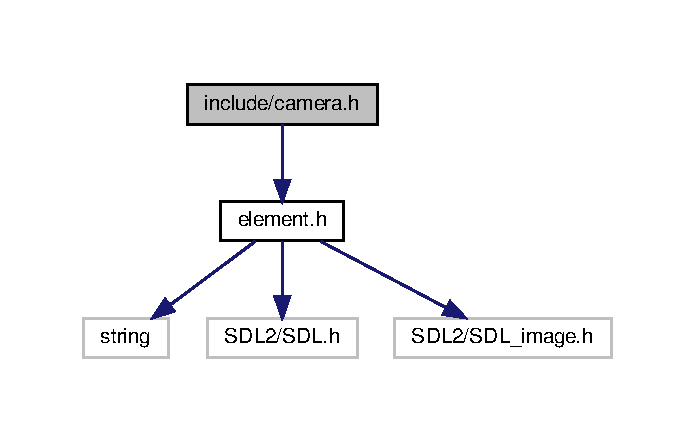
\includegraphics[width=334pt]{camera_8h__incl}
\end{center}
\end{figure}
This graph shows which files directly or indirectly include this file\+:
\nopagebreak
\begin{figure}[H]
\begin{center}
\leavevmode
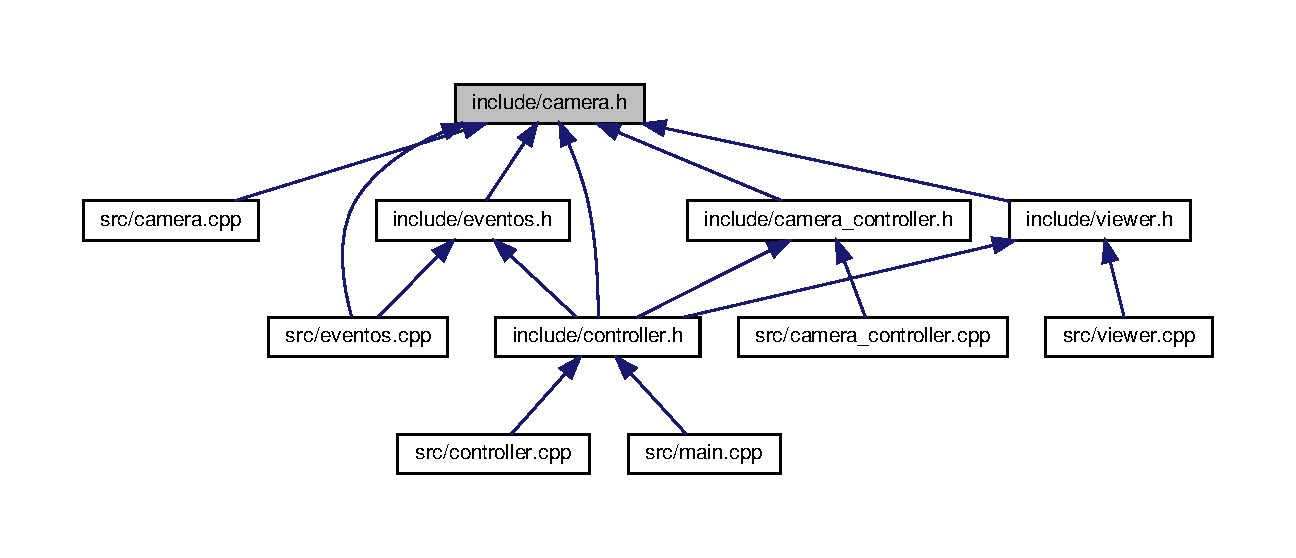
\includegraphics[width=350pt]{camera_8h__dep__incl}
\end{center}
\end{figure}
\subsection*{Classes}
\begin{DoxyCompactItemize}
\item 
class \hyperlink{classCamera}{Camera}
\end{DoxyCompactItemize}

\hypertarget{camera__controller_8h}{}\section{include/camera\+\_\+controller.h File Reference}
\label{camera__controller_8h}\index{include/camera\+\_\+controller.\+h@{include/camera\+\_\+controller.\+h}}
{\ttfamily \#include \char`\"{}camera.\+h\char`\"{}}\newline
{\ttfamily \#include \char`\"{}player.\+h\char`\"{}}\newline
{\ttfamily \#include \char`\"{}map.\+h\char`\"{}}\newline
{\ttfamily \#include $<$stdio.\+h$>$}\newline
{\ttfamily \#include $<$memory$>$}\newline
{\ttfamily \#include $<$iostream$>$}\newline
Include dependency graph for camera\+\_\+controller.\+h\+:
\nopagebreak
\begin{figure}[H]
\begin{center}
\leavevmode
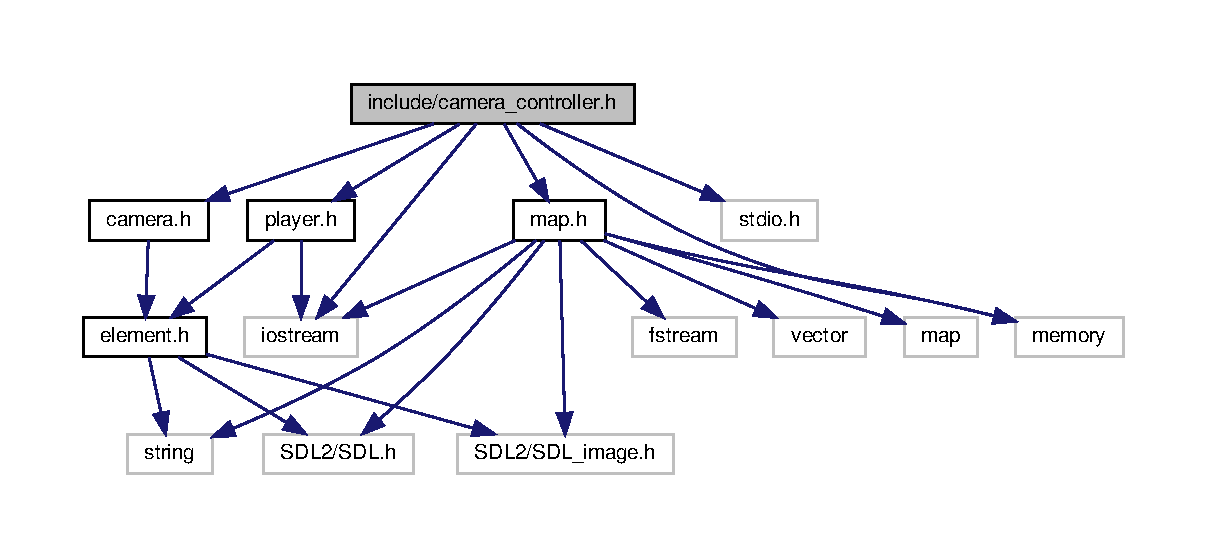
\includegraphics[width=350pt]{camera__controller_8h__incl}
\end{center}
\end{figure}
This graph shows which files directly or indirectly include this file\+:
\nopagebreak
\begin{figure}[H]
\begin{center}
\leavevmode
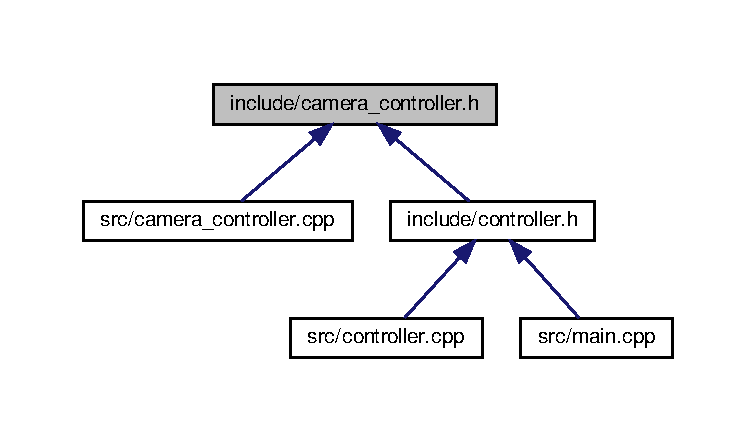
\includegraphics[width=350pt]{camera__controller_8h__dep__incl}
\end{center}
\end{figure}
\subsection*{Classes}
\begin{DoxyCompactItemize}
\item 
class \hyperlink{classCamera__controller}{Camera\+\_\+controller}
\end{DoxyCompactItemize}

\hypertarget{collisionController_8h}{}\section{include/collision\+Controller.h File Reference}
\label{collisionController_8h}\index{include/collision\+Controller.\+h@{include/collision\+Controller.\+h}}
{\ttfamily \#include $<$S\+D\+L2/\+S\+D\+L.\+h$>$}\newline
{\ttfamily \#include $<$string$>$}\newline
{\ttfamily \#include $<$memory$>$}\newline
{\ttfamily \#include $<$map$>$}\newline
{\ttfamily \#include $<$iostream$>$}\newline
{\ttfamily \#include \char`\"{}player.\+h\char`\"{}}\newline
{\ttfamily \#include \char`\"{}map.\+h\char`\"{}}\newline
Include dependency graph for collision\+Controller.\+h\+:
\nopagebreak
\begin{figure}[H]
\begin{center}
\leavevmode
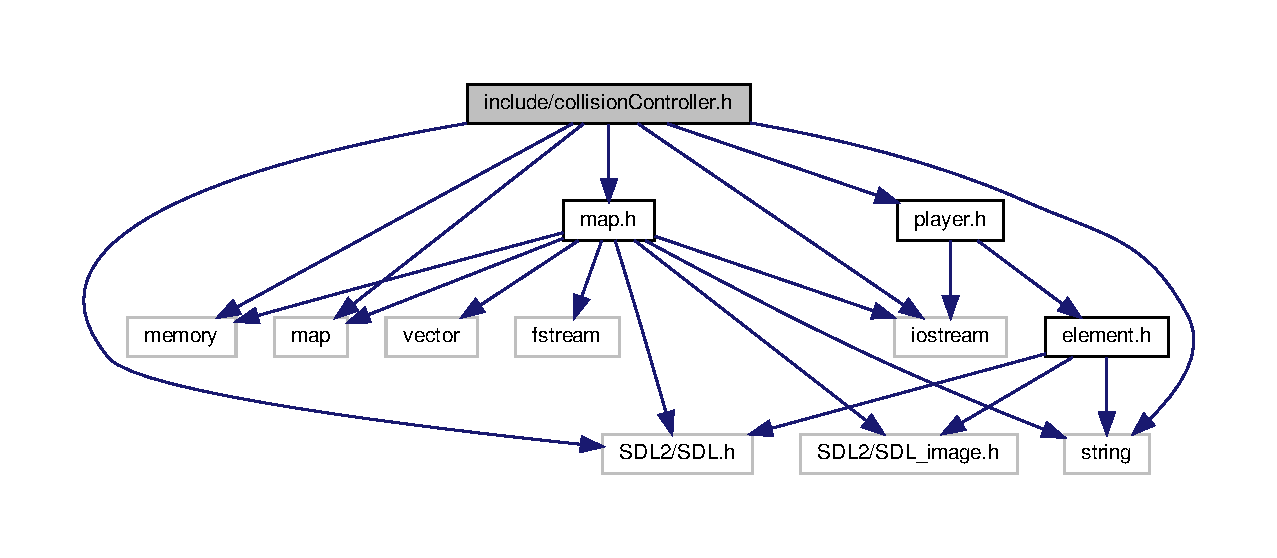
\includegraphics[width=350pt]{collisionController_8h__incl}
\end{center}
\end{figure}
This graph shows which files directly or indirectly include this file\+:
\nopagebreak
\begin{figure}[H]
\begin{center}
\leavevmode
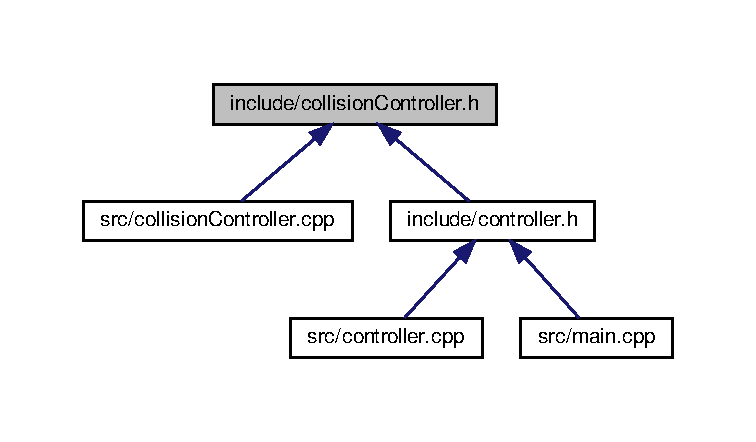
\includegraphics[width=350pt]{collisionController_8h__dep__incl}
\end{center}
\end{figure}
\subsection*{Classes}
\begin{DoxyCompactItemize}
\item 
class \hyperlink{classcollisionController}{collision\+Controller}
\begin{DoxyCompactList}\small\item\em Controle de Colisão. \end{DoxyCompactList}\end{DoxyCompactItemize}

\hypertarget{controller_8h}{}\section{include/controller.h File Reference}
\label{controller_8h}\index{include/controller.\+h@{include/controller.\+h}}
{\ttfamily \#include $<$memory$>$}\newline
{\ttfamily \#include $<$vector$>$}\newline
{\ttfamily \#include $<$S\+D\+L2/\+S\+D\+L.\+h$>$}\newline
{\ttfamily \#include \char`\"{}viewer.\+h\char`\"{}}\newline
{\ttfamily \#include \char`\"{}map.\+h\char`\"{}}\newline
{\ttfamily \#include \char`\"{}element.\+h\char`\"{}}\newline
{\ttfamily \#include \char`\"{}player.\+h\char`\"{}}\newline
{\ttfamily \#include \char`\"{}collision\+Controller.\+h\char`\"{}}\newline
{\ttfamily \#include \char`\"{}camera\+\_\+controller.\+h\char`\"{}}\newline
{\ttfamily \#include \char`\"{}camera.\+h\char`\"{}}\newline
{\ttfamily \#include \char`\"{}porta.\+h\char`\"{}}\newline
{\ttfamily \#include \char`\"{}porta\+\_\+controller.\+h\char`\"{}}\newline
{\ttfamily \#include \char`\"{}eventos.\+h\char`\"{}}\newline
Include dependency graph for controller.\+h\+:
\nopagebreak
\begin{figure}[H]
\begin{center}
\leavevmode
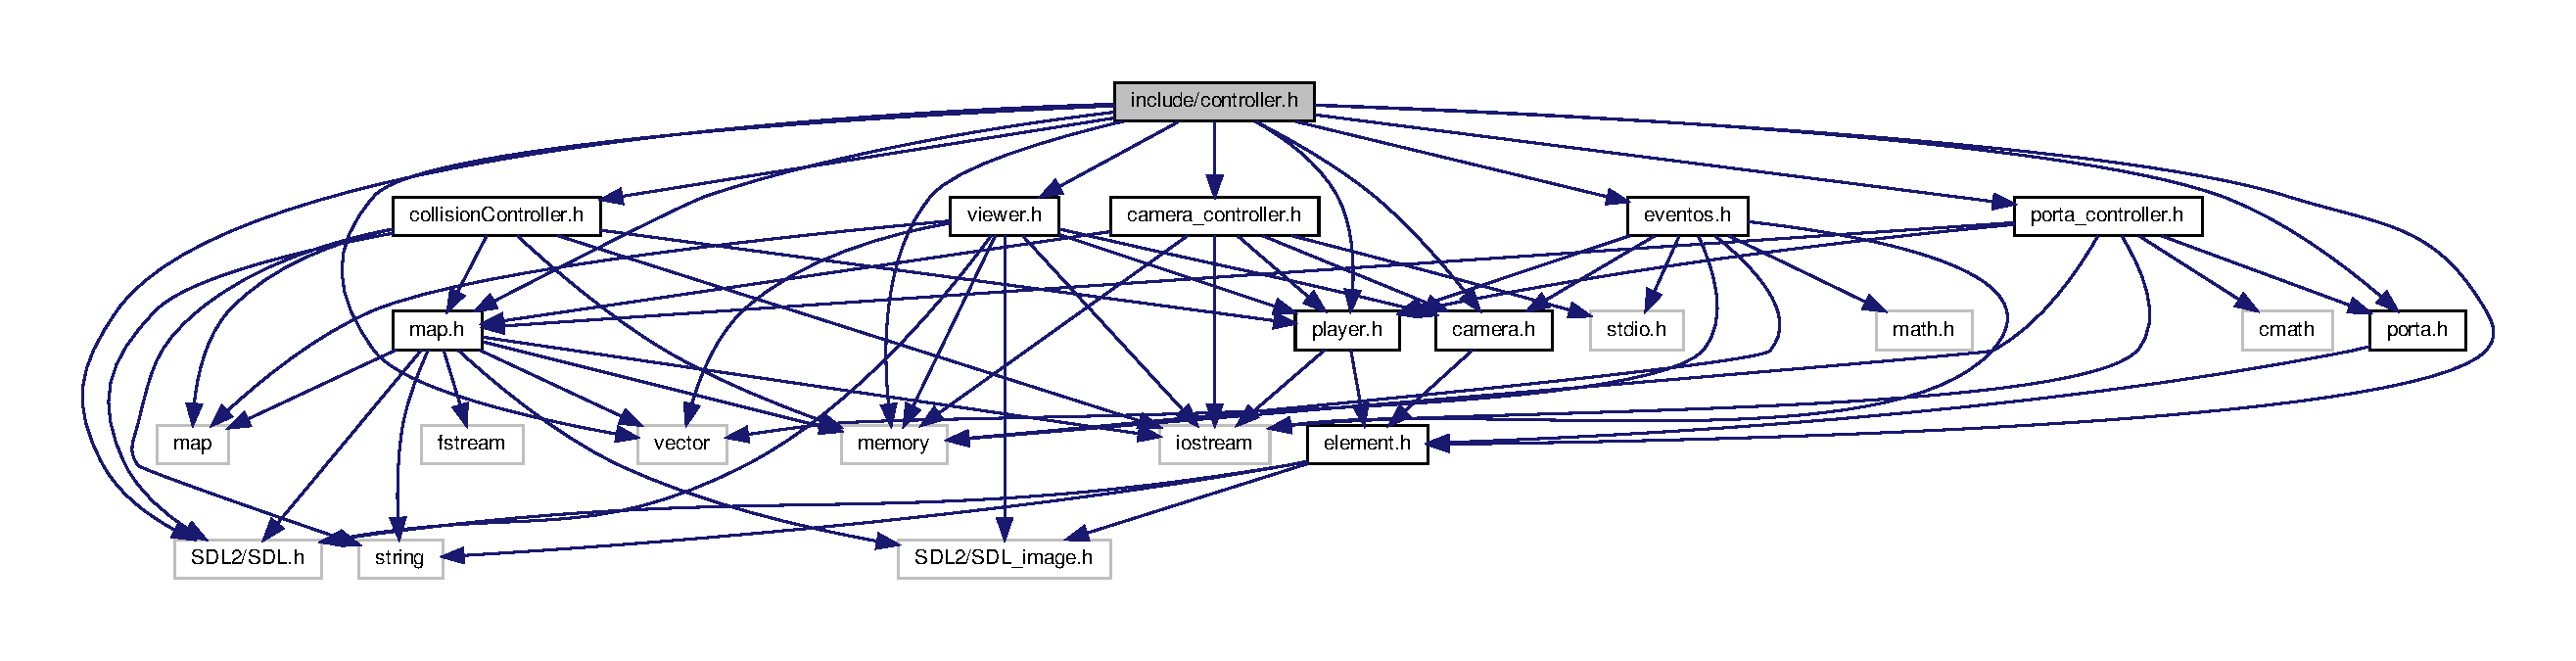
\includegraphics[width=350pt]{controller_8h__incl}
\end{center}
\end{figure}
This graph shows which files directly or indirectly include this file\+:
\nopagebreak
\begin{figure}[H]
\begin{center}
\leavevmode
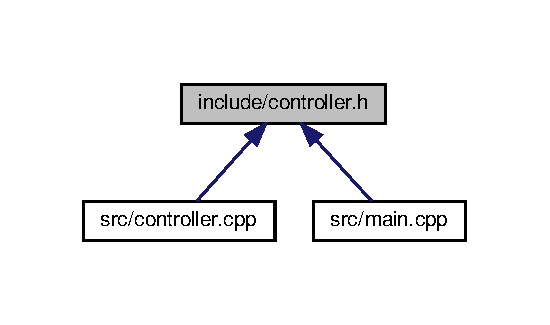
\includegraphics[width=264pt]{controller_8h__dep__incl}
\end{center}
\end{figure}
\subsection*{Classes}
\begin{DoxyCompactItemize}
\item 
class \hyperlink{classController}{Controller}
\begin{DoxyCompactList}\small\item\em Classe para o controller. \end{DoxyCompactList}\end{DoxyCompactItemize}

\hypertarget{element_8h}{}\section{include/element.h File Reference}
\label{element_8h}\index{include/element.\+h@{include/element.\+h}}
{\ttfamily \#include $<$string$>$}\newline
{\ttfamily \#include $<$S\+D\+L2/\+S\+D\+L.\+h$>$}\newline
{\ttfamily \#include $<$S\+D\+L2/\+S\+D\+L\+\_\+image.\+h$>$}\newline
Include dependency graph for element.\+h\+:
\nopagebreak
\begin{figure}[H]
\begin{center}
\leavevmode
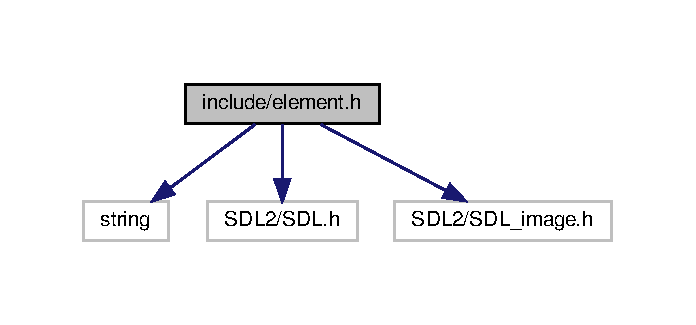
\includegraphics[width=334pt]{element_8h__incl}
\end{center}
\end{figure}
This graph shows which files directly or indirectly include this file\+:
\nopagebreak
\begin{figure}[H]
\begin{center}
\leavevmode
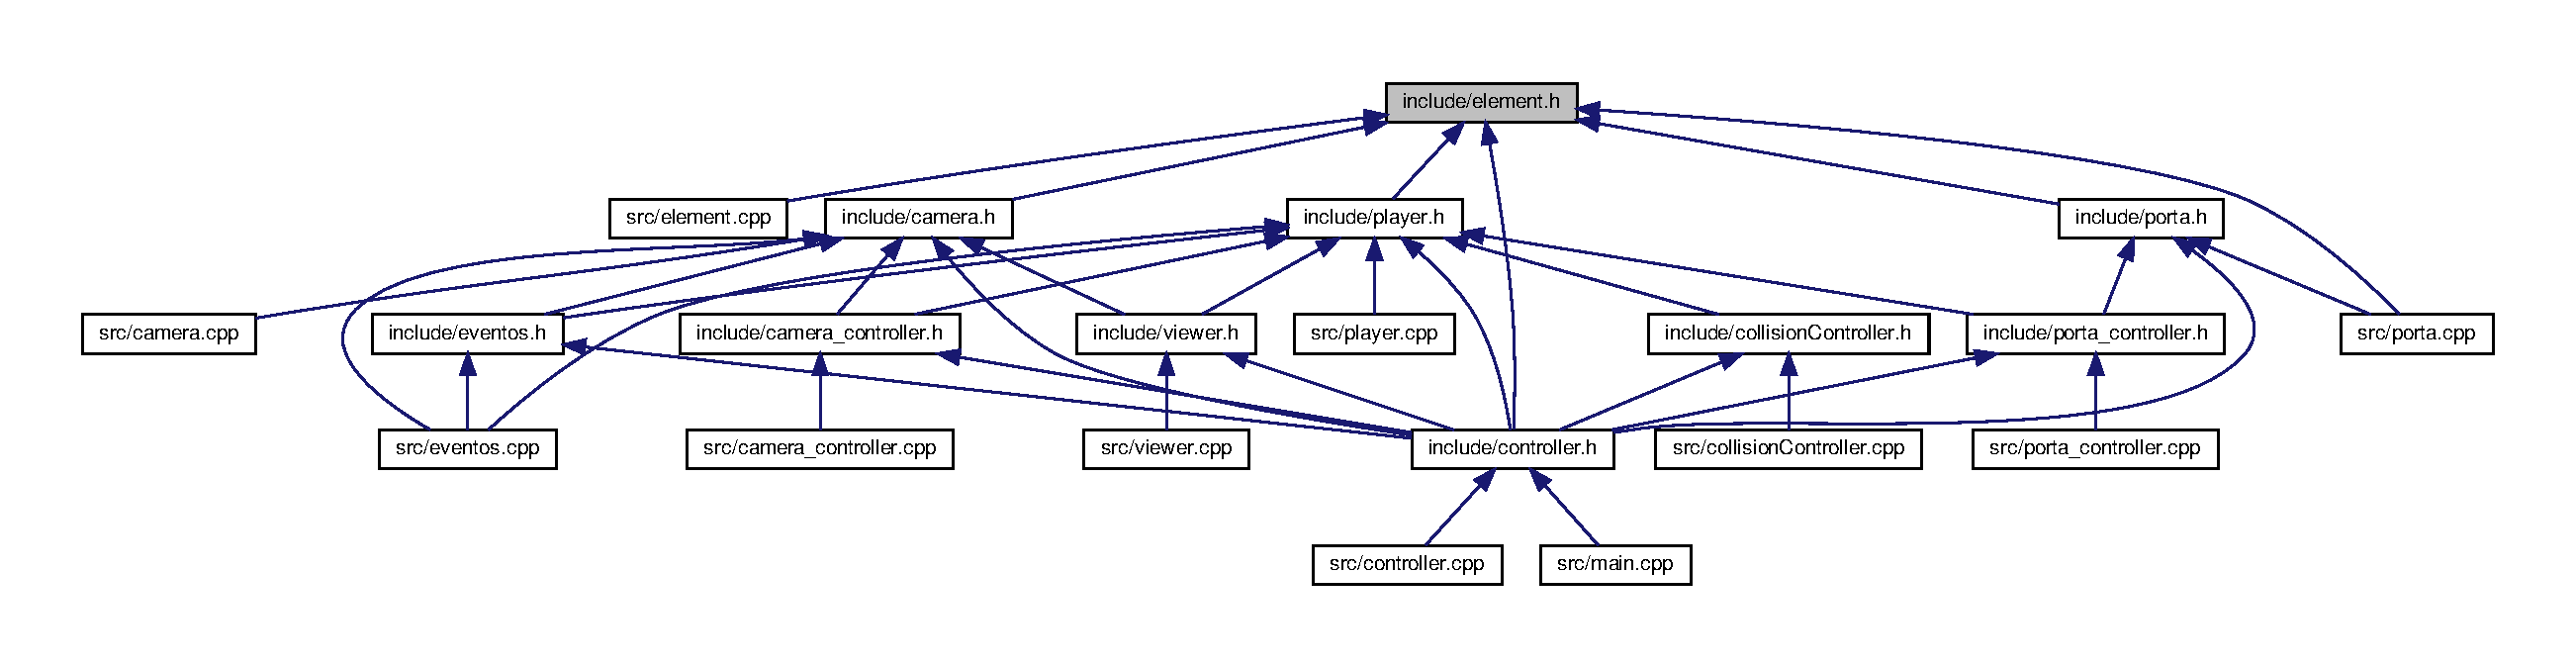
\includegraphics[width=350pt]{element_8h__dep__incl}
\end{center}
\end{figure}
\subsection*{Classes}
\begin{DoxyCompactItemize}
\item 
class \hyperlink{classElement}{Element}
\begin{DoxyCompactList}\small\item\em Classe base de Elementos. \end{DoxyCompactList}\end{DoxyCompactItemize}

\hypertarget{eventos_8h}{}\section{include/eventos.h File Reference}
\label{eventos_8h}\index{include/eventos.\+h@{include/eventos.\+h}}
{\ttfamily \#include $<$stdio.\+h$>$}\newline
{\ttfamily \#include $<$memory$>$}\newline
{\ttfamily \#include $<$iostream$>$}\newline
{\ttfamily \#include $<$vector$>$}\newline
{\ttfamily \#include \char`\"{}player.\+h\char`\"{}}\newline
{\ttfamily \#include \char`\"{}camera.\+h\char`\"{}}\newline
{\ttfamily \#include $<$math.\+h$>$}\newline
Include dependency graph for eventos.\+h\+:
\nopagebreak
\begin{figure}[H]
\begin{center}
\leavevmode
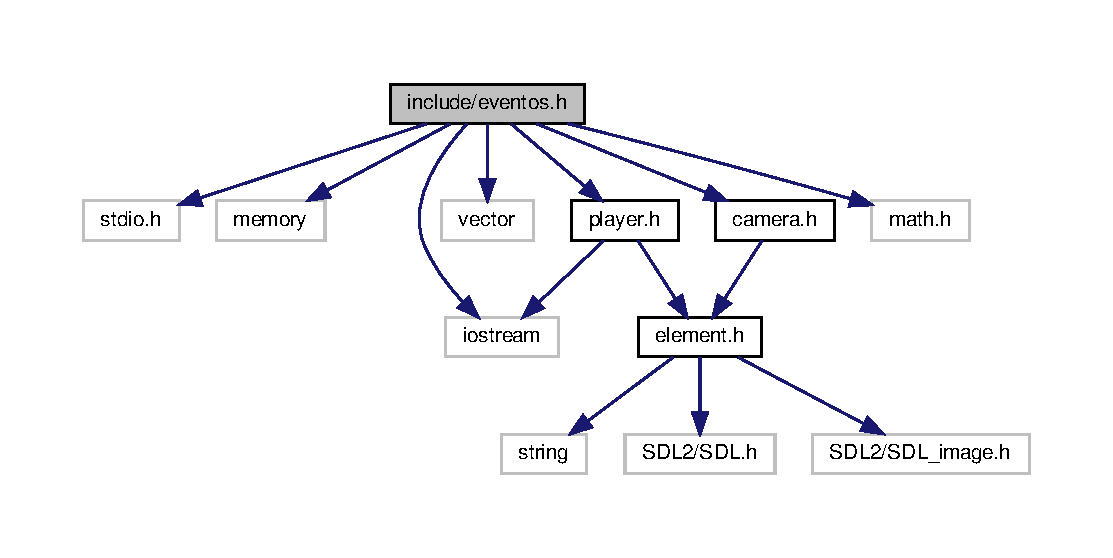
\includegraphics[width=350pt]{eventos_8h__incl}
\end{center}
\end{figure}
This graph shows which files directly or indirectly include this file\+:
\nopagebreak
\begin{figure}[H]
\begin{center}
\leavevmode
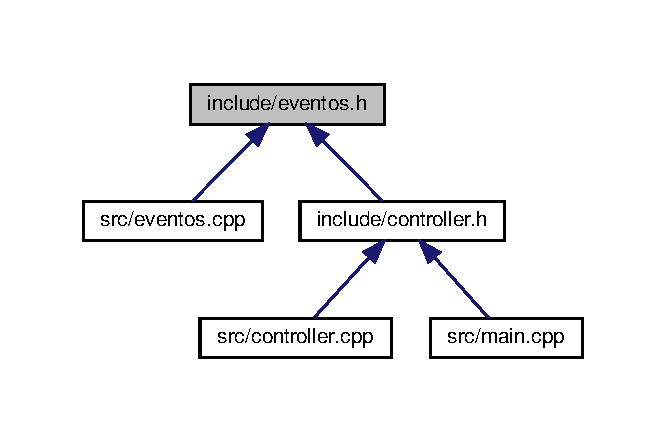
\includegraphics[width=320pt]{eventos_8h__dep__incl}
\end{center}
\end{figure}
\subsection*{Classes}
\begin{DoxyCompactItemize}
\item 
class \hyperlink{classEventos}{Eventos}
\end{DoxyCompactItemize}

\hypertarget{map_8h}{}\section{include/map.h File Reference}
\label{map_8h}\index{include/map.\+h@{include/map.\+h}}
{\ttfamily \#include $<$iostream$>$}\newline
{\ttfamily \#include $<$fstream$>$}\newline
{\ttfamily \#include $<$vector$>$}\newline
{\ttfamily \#include $<$string$>$}\newline
{\ttfamily \#include $<$memory$>$}\newline
{\ttfamily \#include $<$map$>$}\newline
{\ttfamily \#include $<$S\+D\+L2/\+S\+D\+L.\+h$>$}\newline
{\ttfamily \#include $<$S\+D\+L2/\+S\+D\+L\+\_\+image.\+h$>$}\newline
Include dependency graph for map.\+h\+:
\nopagebreak
\begin{figure}[H]
\begin{center}
\leavevmode
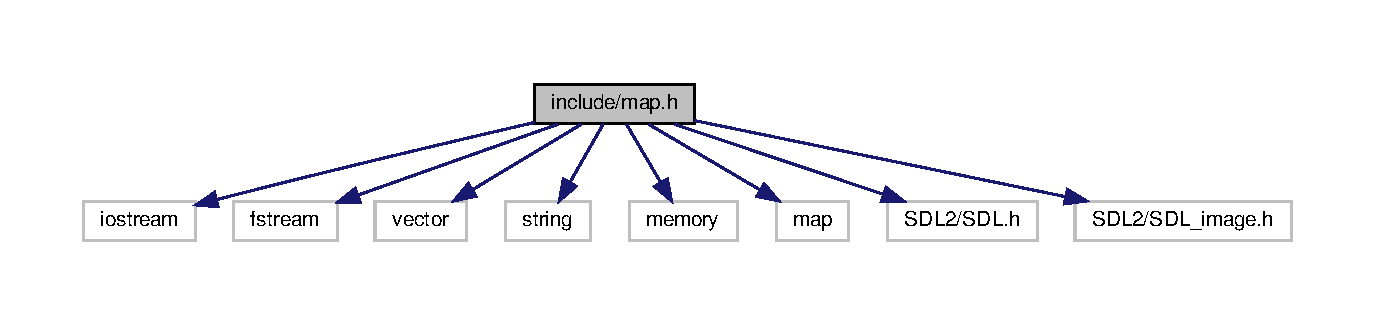
\includegraphics[width=350pt]{map_8h__incl}
\end{center}
\end{figure}
This graph shows which files directly or indirectly include this file\+:
\nopagebreak
\begin{figure}[H]
\begin{center}
\leavevmode
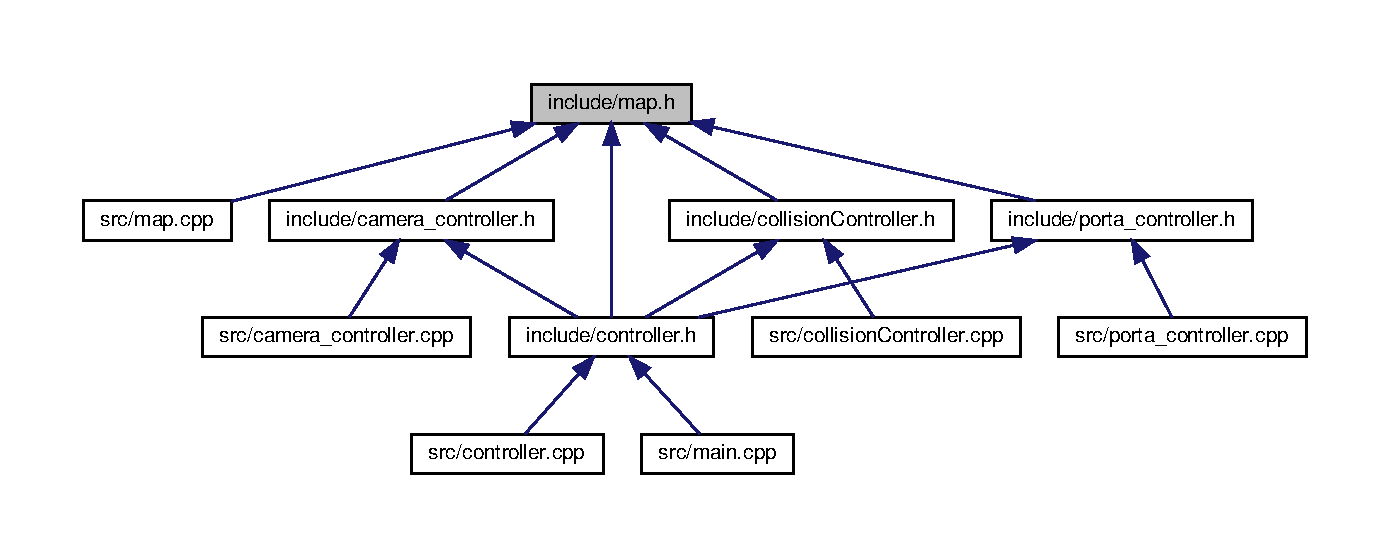
\includegraphics[width=350pt]{map_8h__dep__incl}
\end{center}
\end{figure}
\subsection*{Classes}
\begin{DoxyCompactItemize}
\item 
class \hyperlink{classMap}{Map}
\begin{DoxyCompactList}\small\item\em \hyperlink{classMap}{Map} Class. \end{DoxyCompactList}\end{DoxyCompactItemize}

\hypertarget{player_8h}{}\section{include/player.h File Reference}
\label{player_8h}\index{include/player.\+h@{include/player.\+h}}
{\ttfamily \#include \char`\"{}element.\+h\char`\"{}}\newline
{\ttfamily \#include $<$iostream$>$}\newline
Include dependency graph for player.\+h\+:
\nopagebreak
\begin{figure}[H]
\begin{center}
\leavevmode
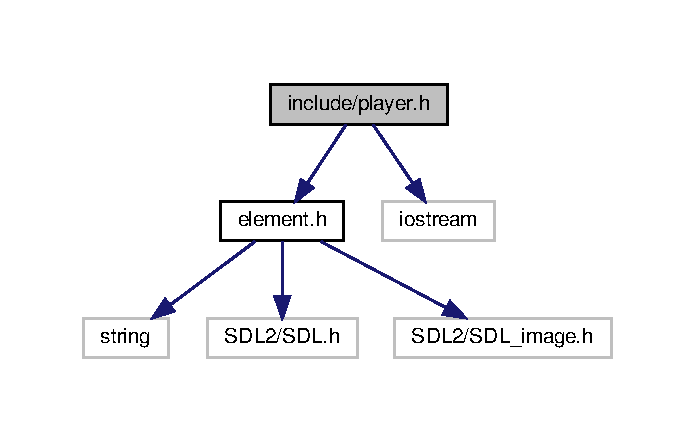
\includegraphics[width=334pt]{player_8h__incl}
\end{center}
\end{figure}
This graph shows which files directly or indirectly include this file\+:
\nopagebreak
\begin{figure}[H]
\begin{center}
\leavevmode
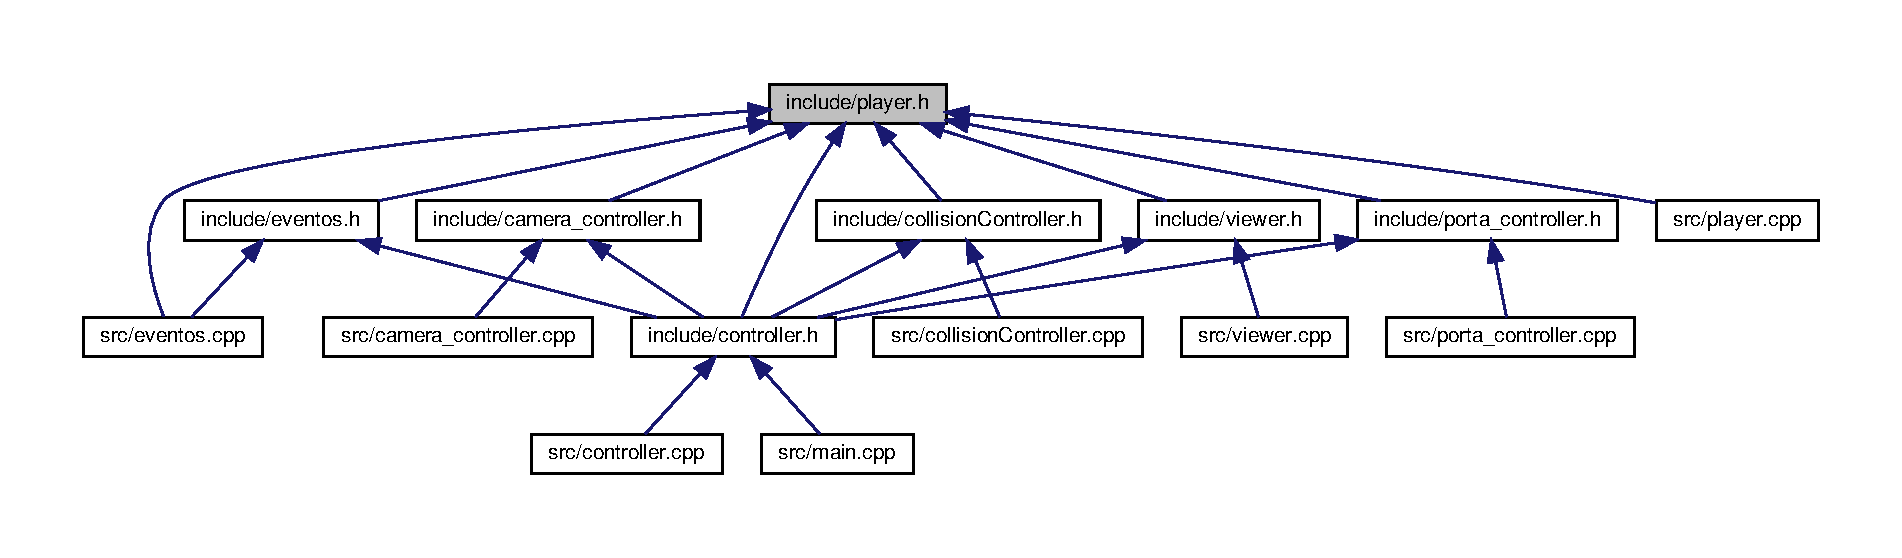
\includegraphics[width=350pt]{player_8h__dep__incl}
\end{center}
\end{figure}
\subsection*{Classes}
\begin{DoxyCompactItemize}
\item 
class \hyperlink{classPlayer}{Player}
\begin{DoxyCompactList}\small\item\em Classe \hyperlink{classPlayer}{Player}. \end{DoxyCompactList}\end{DoxyCompactItemize}

\hypertarget{porta_8h}{}\section{include/porta.h File Reference}
\label{porta_8h}\index{include/porta.\+h@{include/porta.\+h}}
{\ttfamily \#include \char`\"{}element.\+h\char`\"{}}\newline
Include dependency graph for porta.\+h\+:
\nopagebreak
\begin{figure}[H]
\begin{center}
\leavevmode
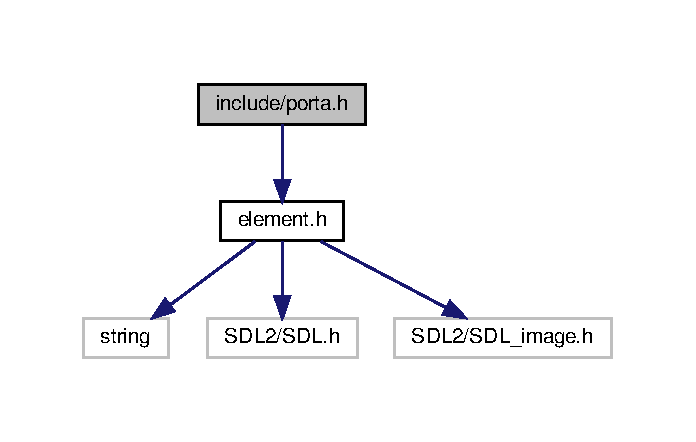
\includegraphics[width=334pt]{porta_8h__incl}
\end{center}
\end{figure}
This graph shows which files directly or indirectly include this file\+:
\nopagebreak
\begin{figure}[H]
\begin{center}
\leavevmode
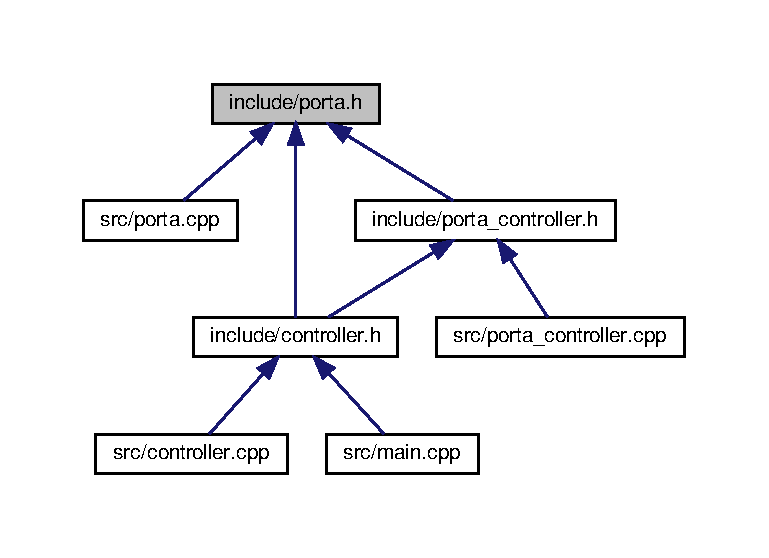
\includegraphics[width=350pt]{porta_8h__dep__incl}
\end{center}
\end{figure}
\subsection*{Classes}
\begin{DoxyCompactItemize}
\item 
class \hyperlink{classPorta}{Porta}
\end{DoxyCompactItemize}

\hypertarget{porta__controller_8h}{}\section{include/porta\+\_\+controller.h File Reference}
\label{porta__controller_8h}\index{include/porta\+\_\+controller.\+h@{include/porta\+\_\+controller.\+h}}
{\ttfamily \#include $<$iostream$>$}\newline
{\ttfamily \#include $<$memory$>$}\newline
{\ttfamily \#include $<$cmath$>$}\newline
{\ttfamily \#include \char`\"{}player.\+h\char`\"{}}\newline
{\ttfamily \#include \char`\"{}porta.\+h\char`\"{}}\newline
{\ttfamily \#include \char`\"{}map.\+h\char`\"{}}\newline
Include dependency graph for porta\+\_\+controller.\+h\+:
\nopagebreak
\begin{figure}[H]
\begin{center}
\leavevmode
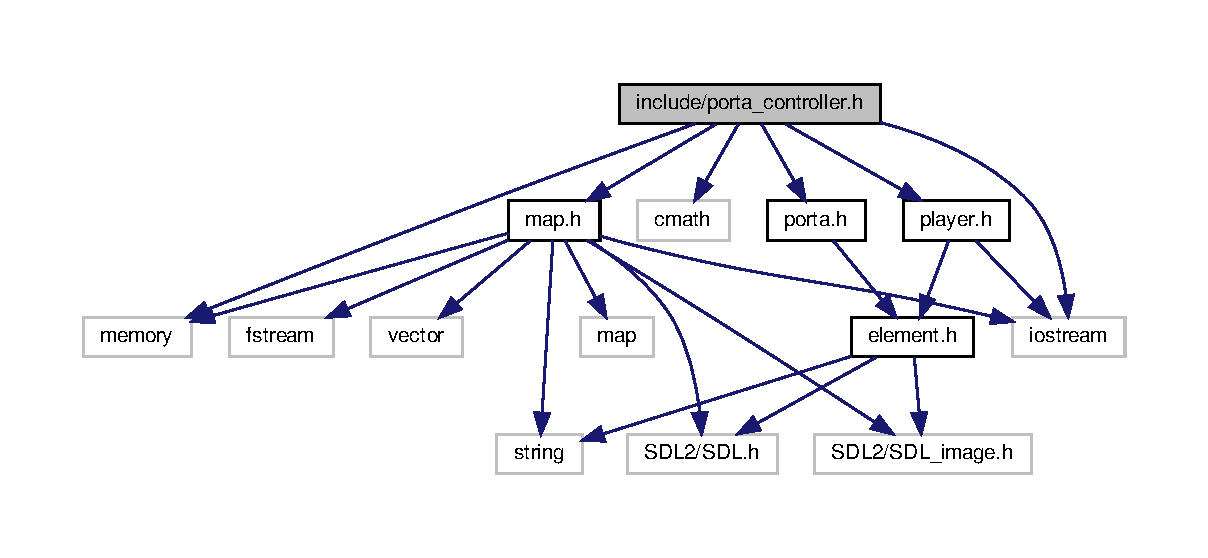
\includegraphics[width=350pt]{porta__controller_8h__incl}
\end{center}
\end{figure}
This graph shows which files directly or indirectly include this file\+:
\nopagebreak
\begin{figure}[H]
\begin{center}
\leavevmode
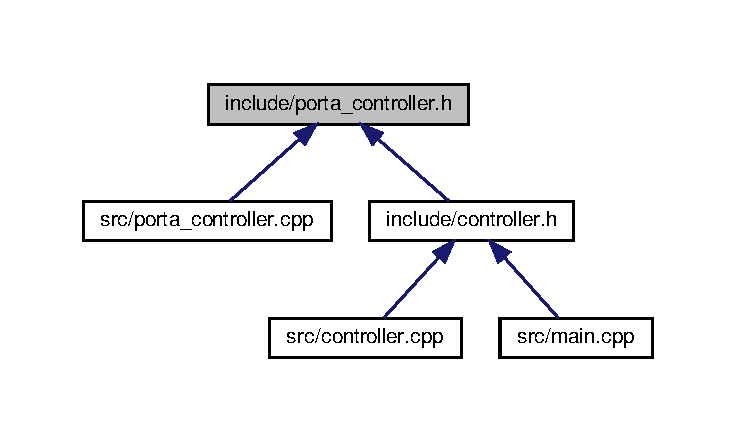
\includegraphics[width=350pt]{porta__controller_8h__dep__incl}
\end{center}
\end{figure}
\subsection*{Classes}
\begin{DoxyCompactItemize}
\item 
class \hyperlink{classPorta__controller}{Porta\+\_\+controller}
\end{DoxyCompactItemize}

\hypertarget{viewer_8h}{}\section{include/viewer.h File Reference}
\label{viewer_8h}\index{include/viewer.\+h@{include/viewer.\+h}}
{\ttfamily \#include $<$memory$>$}\newline
{\ttfamily \#include $<$iostream$>$}\newline
{\ttfamily \#include $<$map$>$}\newline
{\ttfamily \#include $<$vector$>$}\newline
{\ttfamily \#include $<$S\+D\+L2/\+S\+D\+L.\+h$>$}\newline
{\ttfamily \#include $<$S\+D\+L2/\+S\+D\+L\+\_\+image.\+h$>$}\newline
{\ttfamily \#include \char`\"{}player.\+h\char`\"{}}\newline
{\ttfamily \#include \char`\"{}camera.\+h\char`\"{}}\newline
Include dependency graph for viewer.\+h\+:
\nopagebreak
\begin{figure}[H]
\begin{center}
\leavevmode
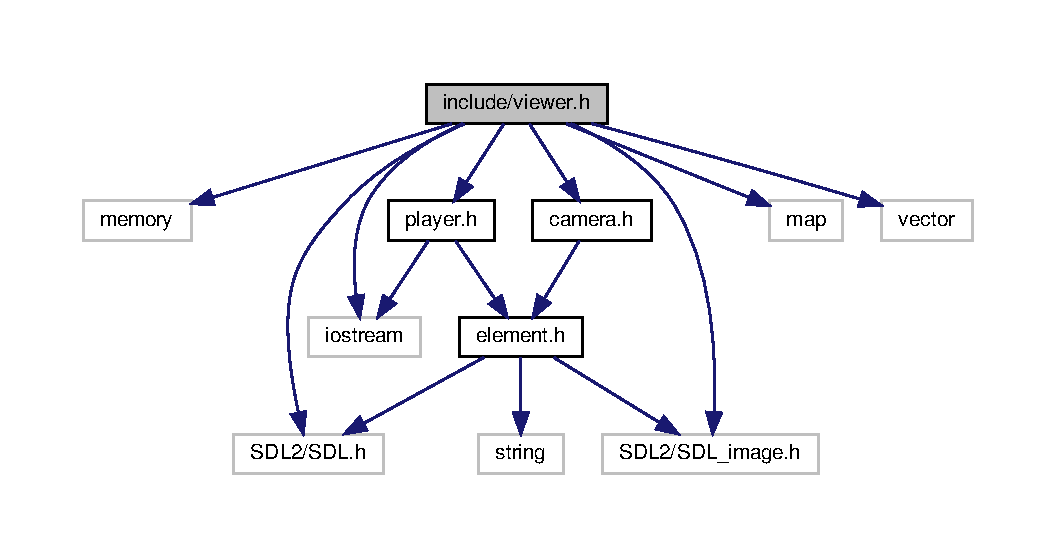
\includegraphics[width=350pt]{viewer_8h__incl}
\end{center}
\end{figure}
This graph shows which files directly or indirectly include this file\+:
\nopagebreak
\begin{figure}[H]
\begin{center}
\leavevmode
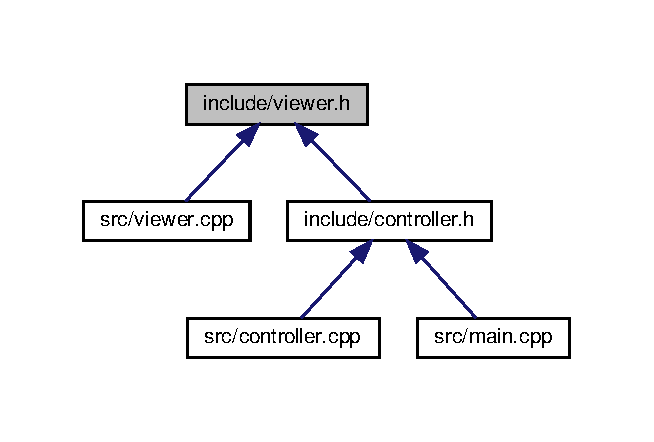
\includegraphics[width=314pt]{viewer_8h__dep__incl}
\end{center}
\end{figure}
\subsection*{Classes}
\begin{DoxyCompactItemize}
\item 
class \hyperlink{classViewer}{Viewer}
\end{DoxyCompactItemize}

\hypertarget{camera_8cpp}{}\section{src/camera.cpp File Reference}
\label{camera_8cpp}\index{src/camera.\+cpp@{src/camera.\+cpp}}
{\ttfamily \#include \char`\"{}camera.\+h\char`\"{}}\newline
Include dependency graph for camera.\+cpp\+:
\nopagebreak
\begin{figure}[H]
\begin{center}
\leavevmode
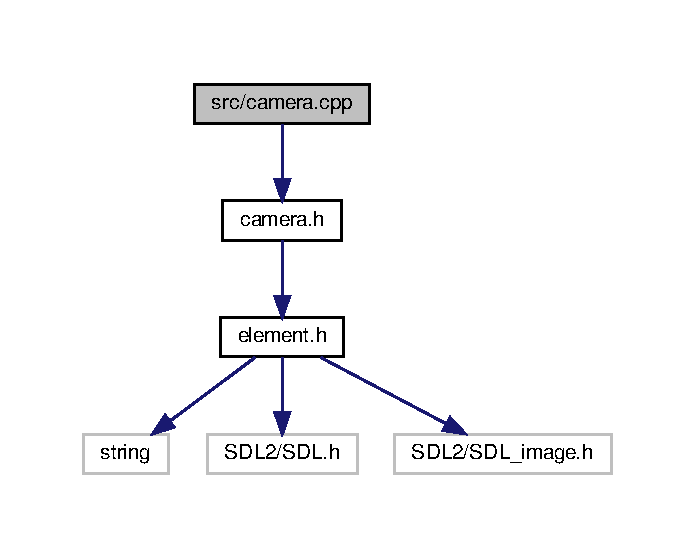
\includegraphics[width=334pt]{camera_8cpp__incl}
\end{center}
\end{figure}

\hypertarget{camera__controller_8cpp}{}\section{src/camera\+\_\+controller.cpp File Reference}
\label{camera__controller_8cpp}\index{src/camera\+\_\+controller.\+cpp@{src/camera\+\_\+controller.\+cpp}}
{\ttfamily \#include \char`\"{}camera\+\_\+controller.\+h\char`\"{}}\newline
Include dependency graph for camera\+\_\+controller.\+cpp\+:
\nopagebreak
\begin{figure}[H]
\begin{center}
\leavevmode
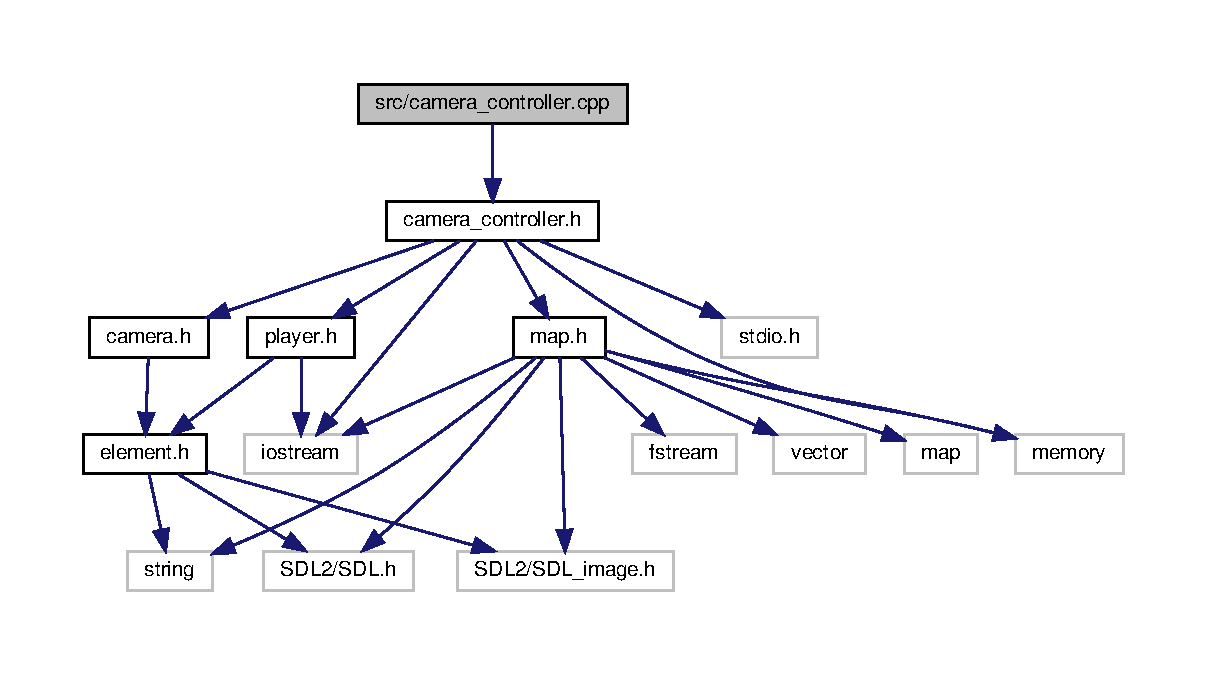
\includegraphics[width=350pt]{camera__controller_8cpp__incl}
\end{center}
\end{figure}

\hypertarget{collisionController_8cpp}{}\section{src/collision\+Controller.cpp File Reference}
\label{collisionController_8cpp}\index{src/collision\+Controller.\+cpp@{src/collision\+Controller.\+cpp}}
{\ttfamily \#include \char`\"{}collision\+Controller.\+h\char`\"{}}\newline
Include dependency graph for collision\+Controller.\+cpp\+:
\nopagebreak
\begin{figure}[H]
\begin{center}
\leavevmode
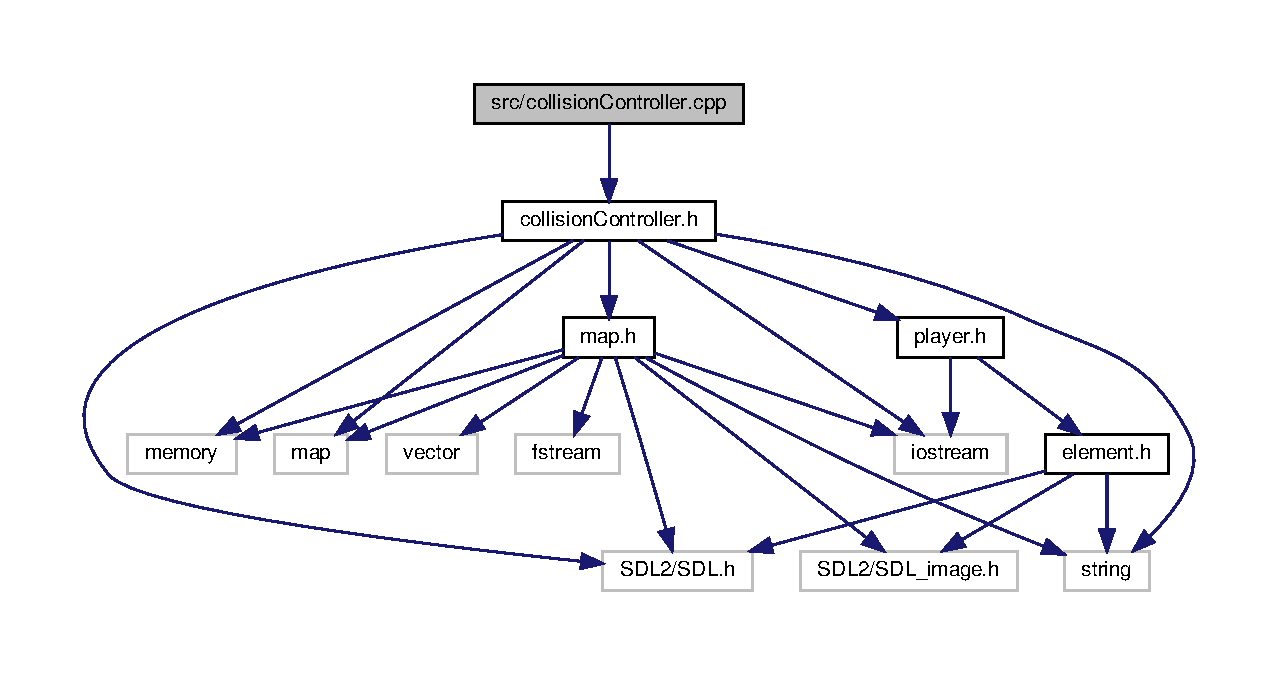
\includegraphics[width=350pt]{collisionController_8cpp__incl}
\end{center}
\end{figure}

\hypertarget{controller_8cpp}{}\section{src/controller.cpp File Reference}
\label{controller_8cpp}\index{src/controller.\+cpp@{src/controller.\+cpp}}
{\ttfamily \#include \char`\"{}controller.\+h\char`\"{}}\newline
Include dependency graph for controller.\+cpp\+:
\nopagebreak
\begin{figure}[H]
\begin{center}
\leavevmode
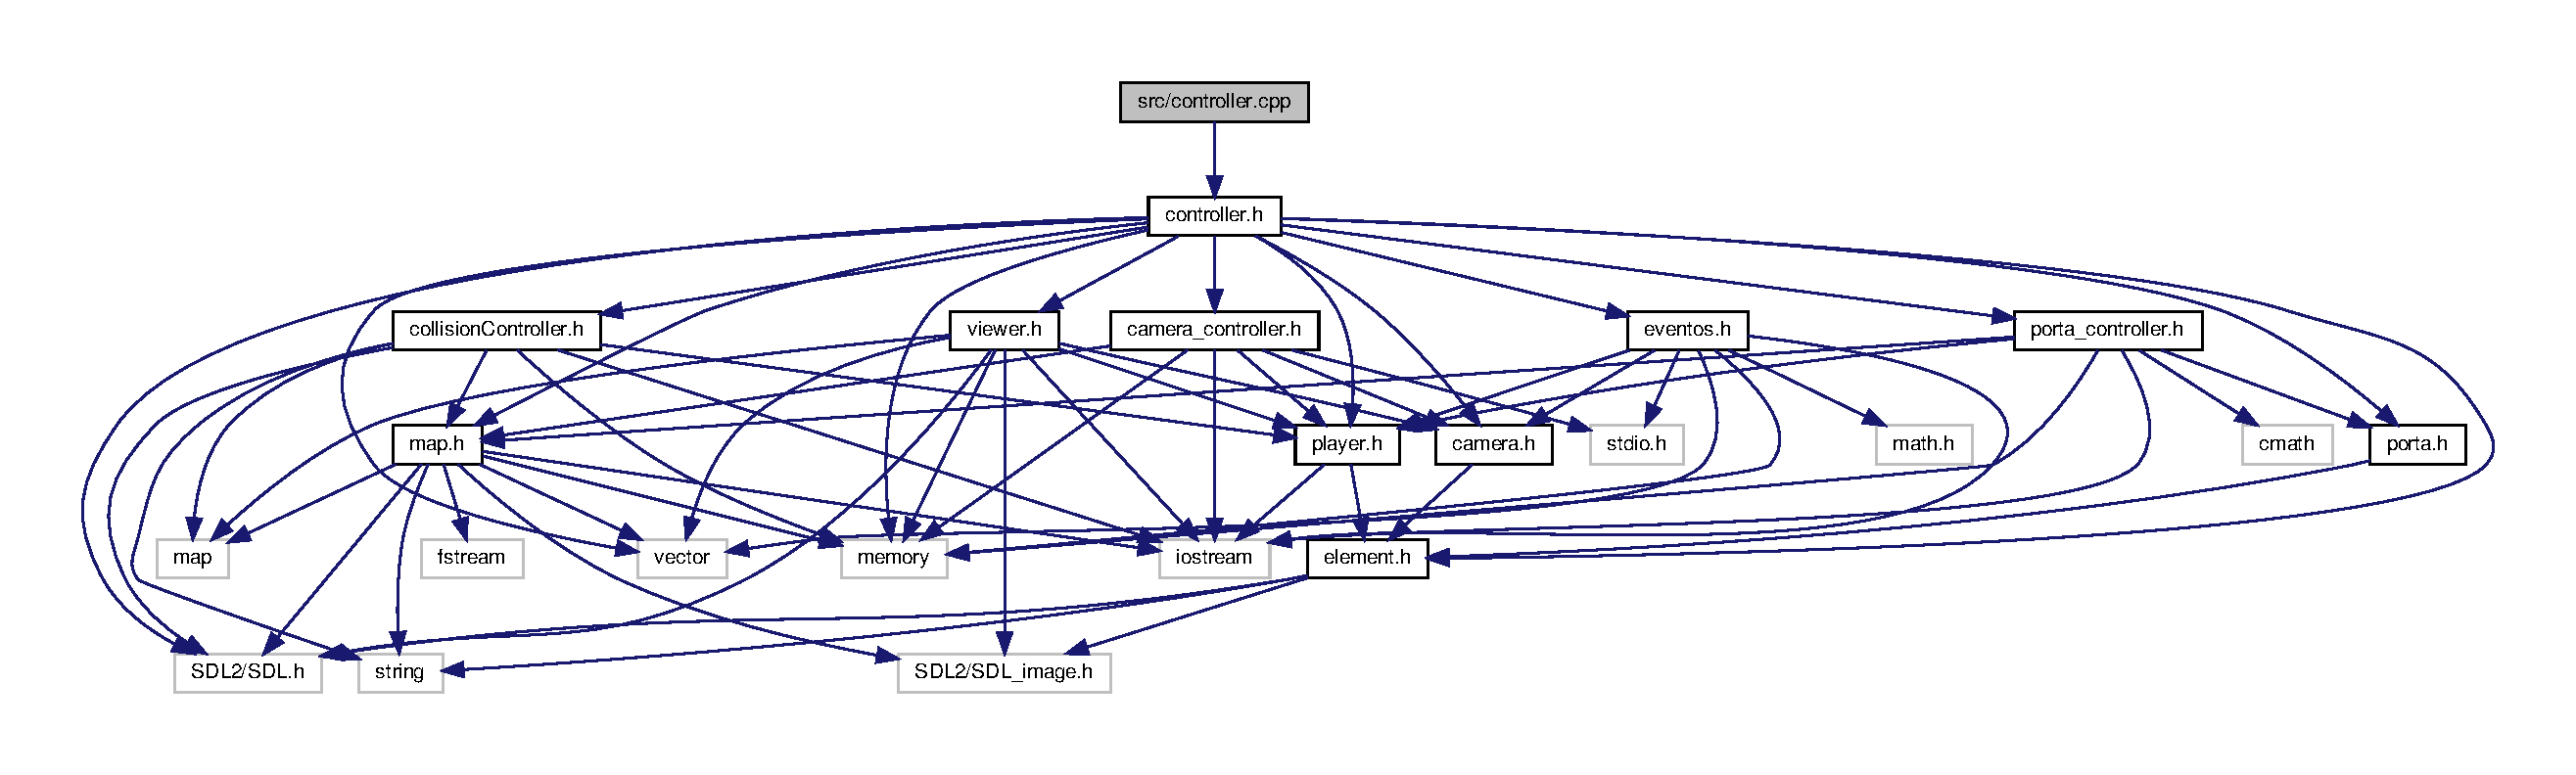
\includegraphics[width=350pt]{controller_8cpp__incl}
\end{center}
\end{figure}

\hypertarget{element_8cpp}{}\section{src/element.cpp File Reference}
\label{element_8cpp}\index{src/element.\+cpp@{src/element.\+cpp}}
{\ttfamily \#include \char`\"{}element.\+h\char`\"{}}\newline
Include dependency graph for element.\+cpp\+:
\nopagebreak
\begin{figure}[H]
\begin{center}
\leavevmode
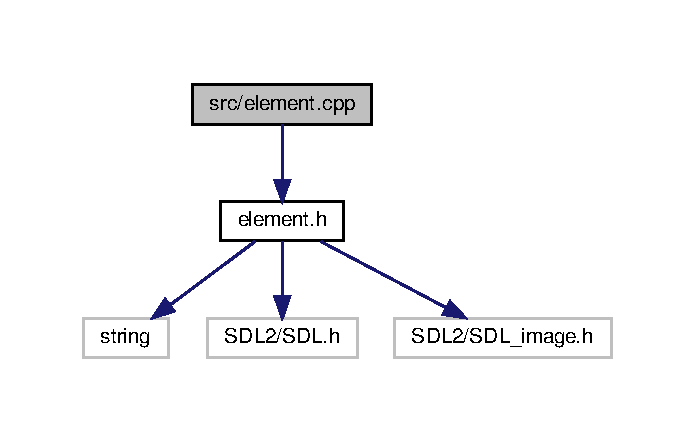
\includegraphics[width=334pt]{element_8cpp__incl}
\end{center}
\end{figure}

\hypertarget{eventos_8cpp}{}\section{src/eventos.cpp File Reference}
\label{eventos_8cpp}\index{src/eventos.\+cpp@{src/eventos.\+cpp}}
{\ttfamily \#include $<$stdio.\+h$>$}\newline
{\ttfamily \#include $<$memory$>$}\newline
{\ttfamily \#include $<$iostream$>$}\newline
{\ttfamily \#include $<$vector$>$}\newline
{\ttfamily \#include \char`\"{}eventos.\+h\char`\"{}}\newline
{\ttfamily \#include \char`\"{}player.\+h\char`\"{}}\newline
{\ttfamily \#include \char`\"{}camera.\+h\char`\"{}}\newline
Include dependency graph for eventos.\+cpp\+:
\nopagebreak
\begin{figure}[H]
\begin{center}
\leavevmode
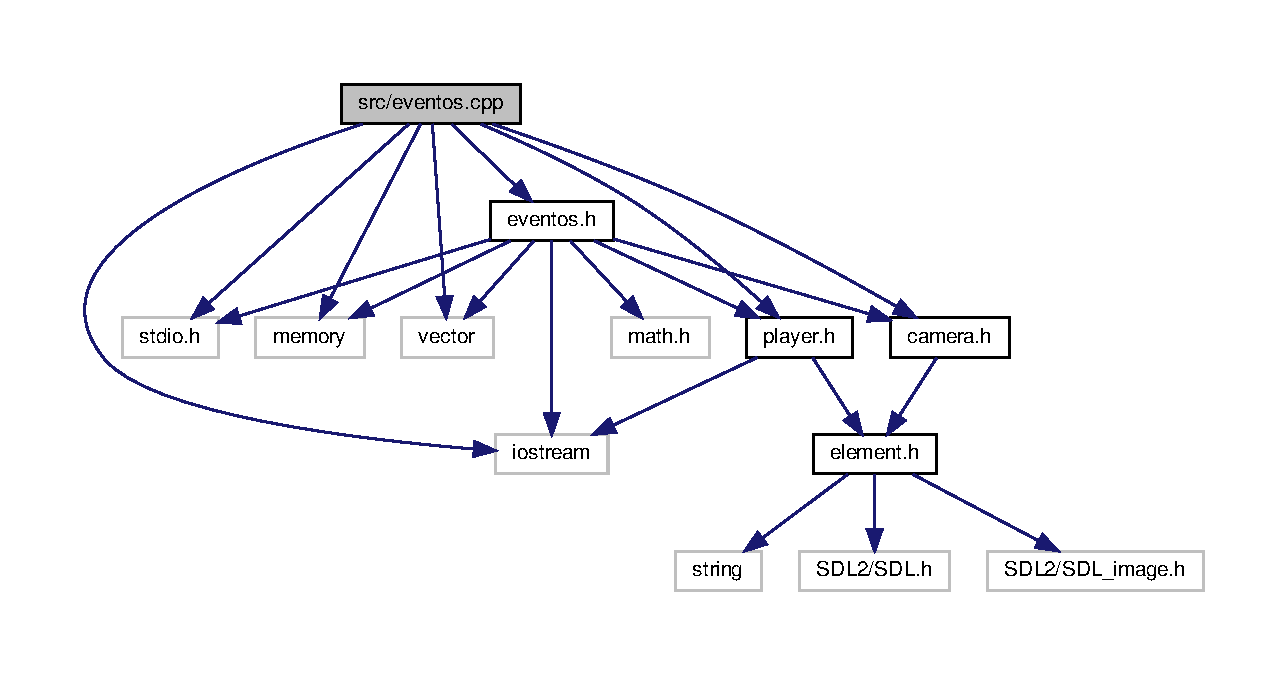
\includegraphics[width=350pt]{eventos_8cpp__incl}
\end{center}
\end{figure}

\hypertarget{main_8cpp}{}\section{src/main.cpp File Reference}
\label{main_8cpp}\index{src/main.\+cpp@{src/main.\+cpp}}
{\ttfamily \#include \char`\"{}controller.\+h\char`\"{}}\newline
Include dependency graph for main.\+cpp\+:
\nopagebreak
\begin{figure}[H]
\begin{center}
\leavevmode
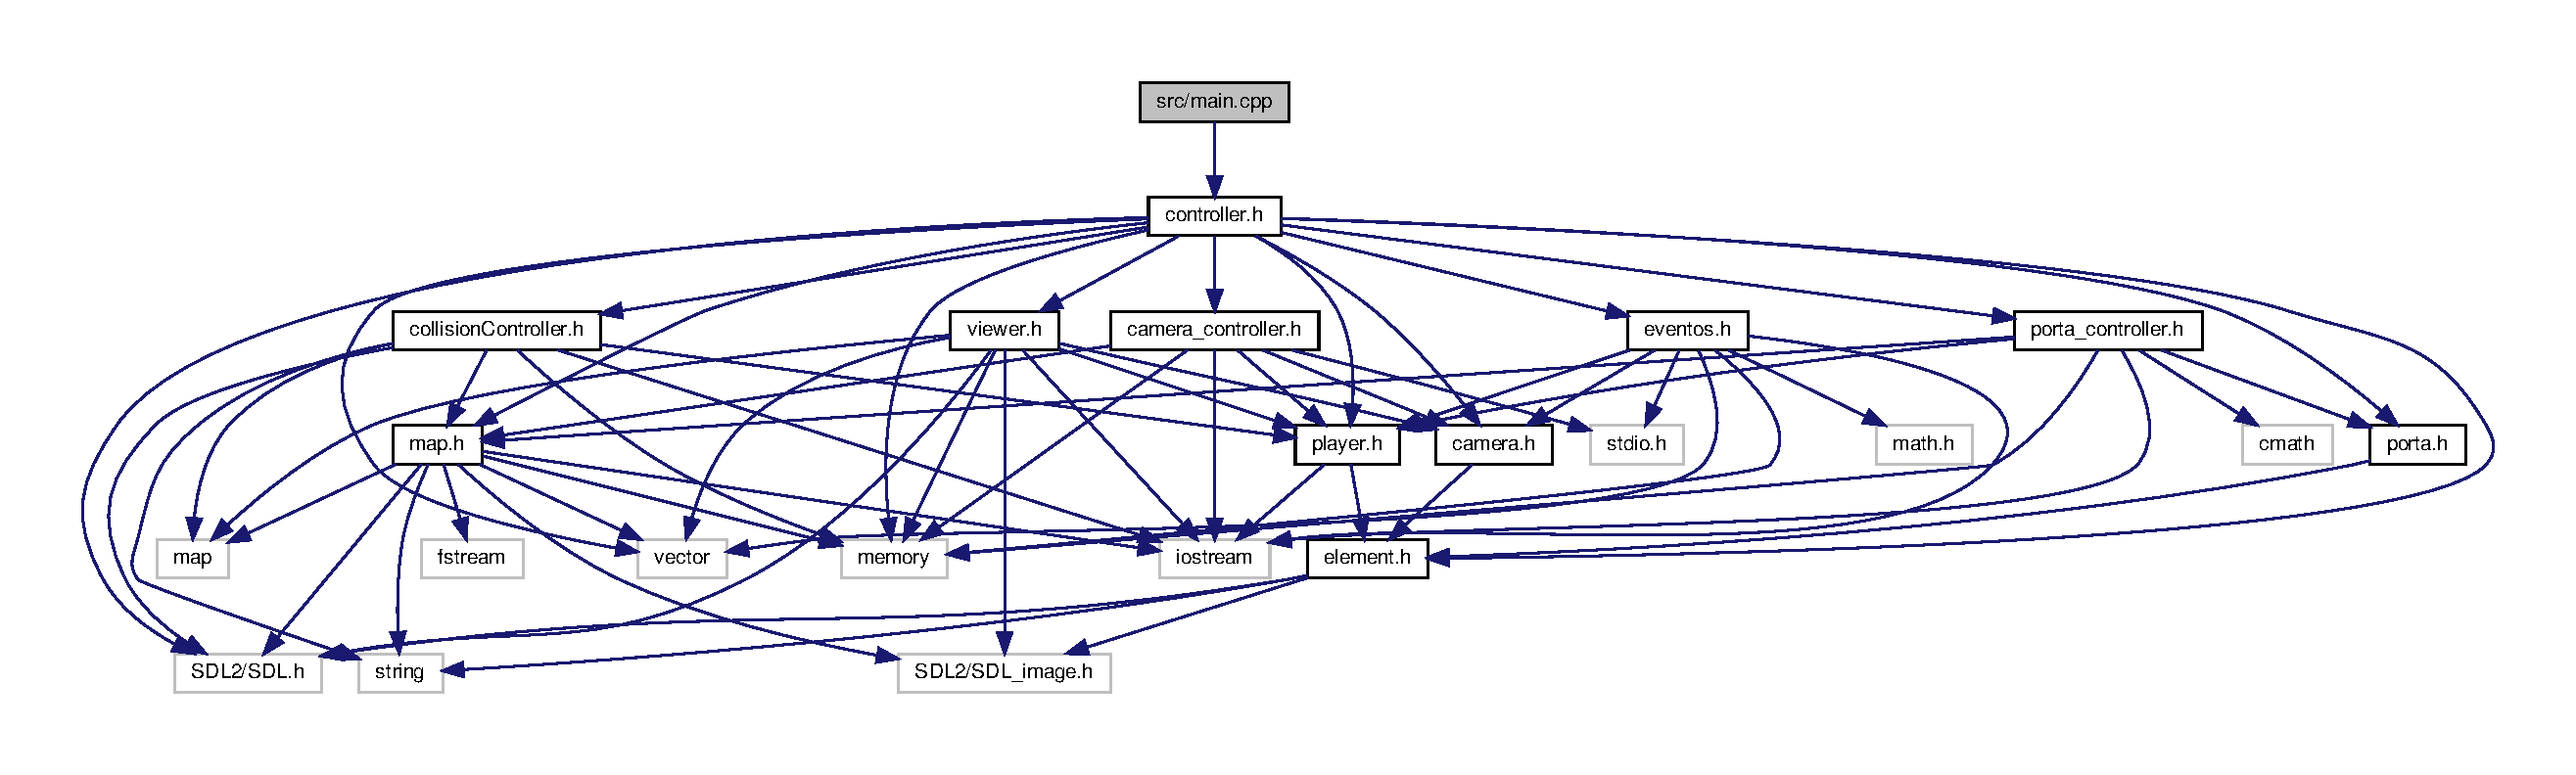
\includegraphics[width=350pt]{main_8cpp__incl}
\end{center}
\end{figure}
\subsection*{Functions}
\begin{DoxyCompactItemize}
\item 
int \hyperlink{main_8cpp_ae66f6b31b5ad750f1fe042a706a4e3d4}{main} ()
\end{DoxyCompactItemize}


\subsection{Function Documentation}
\mbox{\Hypertarget{main_8cpp_ae66f6b31b5ad750f1fe042a706a4e3d4}\label{main_8cpp_ae66f6b31b5ad750f1fe042a706a4e3d4}} 
\index{main.\+cpp@{main.\+cpp}!main@{main}}
\index{main@{main}!main.\+cpp@{main.\+cpp}}
\subsubsection{\texorpdfstring{main()}{main()}}
{\footnotesize\ttfamily int main (\begin{DoxyParamCaption}{ }\end{DoxyParamCaption})}


\hypertarget{map_8cpp}{}\section{src/map.cpp File Reference}
\label{map_8cpp}\index{src/map.\+cpp@{src/map.\+cpp}}
{\ttfamily \#include \char`\"{}map.\+h\char`\"{}}\newline
Include dependency graph for map.\+cpp\+:
\nopagebreak
\begin{figure}[H]
\begin{center}
\leavevmode
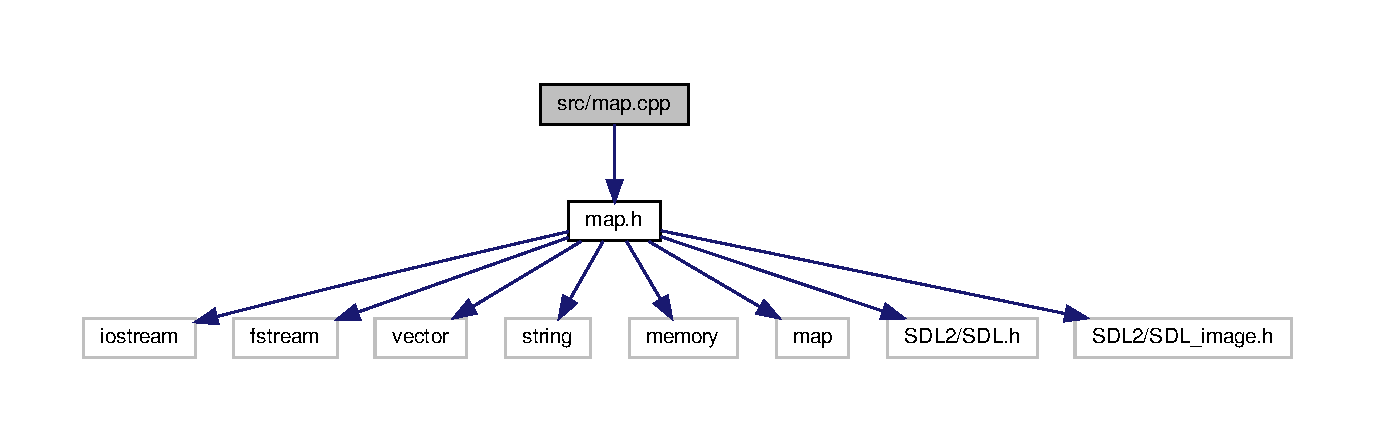
\includegraphics[width=350pt]{map_8cpp__incl}
\end{center}
\end{figure}

\hypertarget{player_8cpp}{}\section{src/player.cpp File Reference}
\label{player_8cpp}\index{src/player.\+cpp@{src/player.\+cpp}}
{\ttfamily \#include \char`\"{}player.\+h\char`\"{}}\newline
Include dependency graph for player.\+cpp\+:
\nopagebreak
\begin{figure}[H]
\begin{center}
\leavevmode
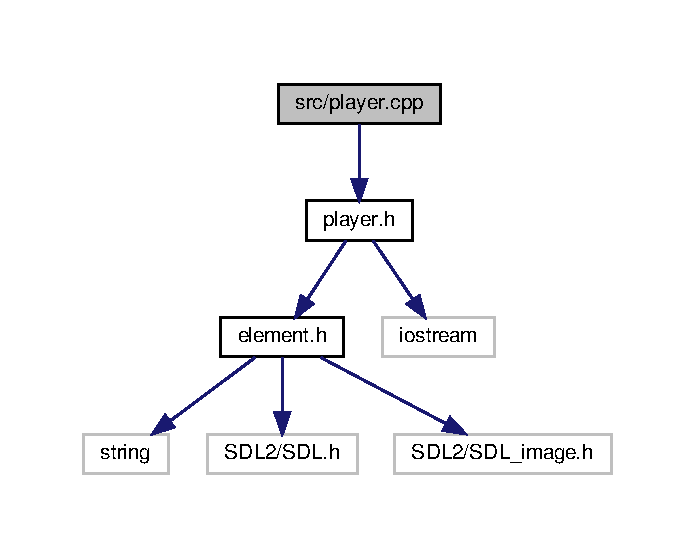
\includegraphics[width=334pt]{player_8cpp__incl}
\end{center}
\end{figure}

\hypertarget{porta_8cpp}{}\section{src/porta.cpp File Reference}
\label{porta_8cpp}\index{src/porta.\+cpp@{src/porta.\+cpp}}
{\ttfamily \#include \char`\"{}porta.\+h\char`\"{}}\newline
{\ttfamily \#include \char`\"{}element.\+h\char`\"{}}\newline
Include dependency graph for porta.\+cpp\+:
\nopagebreak
\begin{figure}[H]
\begin{center}
\leavevmode
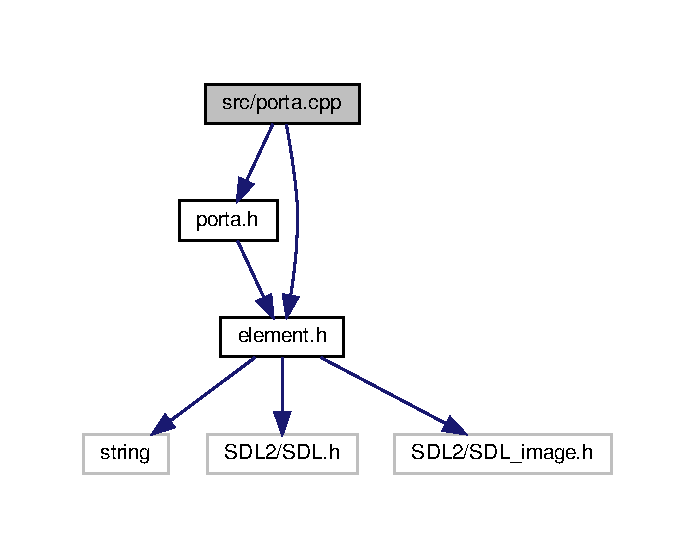
\includegraphics[width=334pt]{porta_8cpp__incl}
\end{center}
\end{figure}

\hypertarget{porta__controller_8cpp}{}\section{src/porta\+\_\+controller.cpp File Reference}
\label{porta__controller_8cpp}\index{src/porta\+\_\+controller.\+cpp@{src/porta\+\_\+controller.\+cpp}}
{\ttfamily \#include \char`\"{}porta\+\_\+controller.\+h\char`\"{}}\newline
Include dependency graph for porta\+\_\+controller.\+cpp\+:
\nopagebreak
\begin{figure}[H]
\begin{center}
\leavevmode
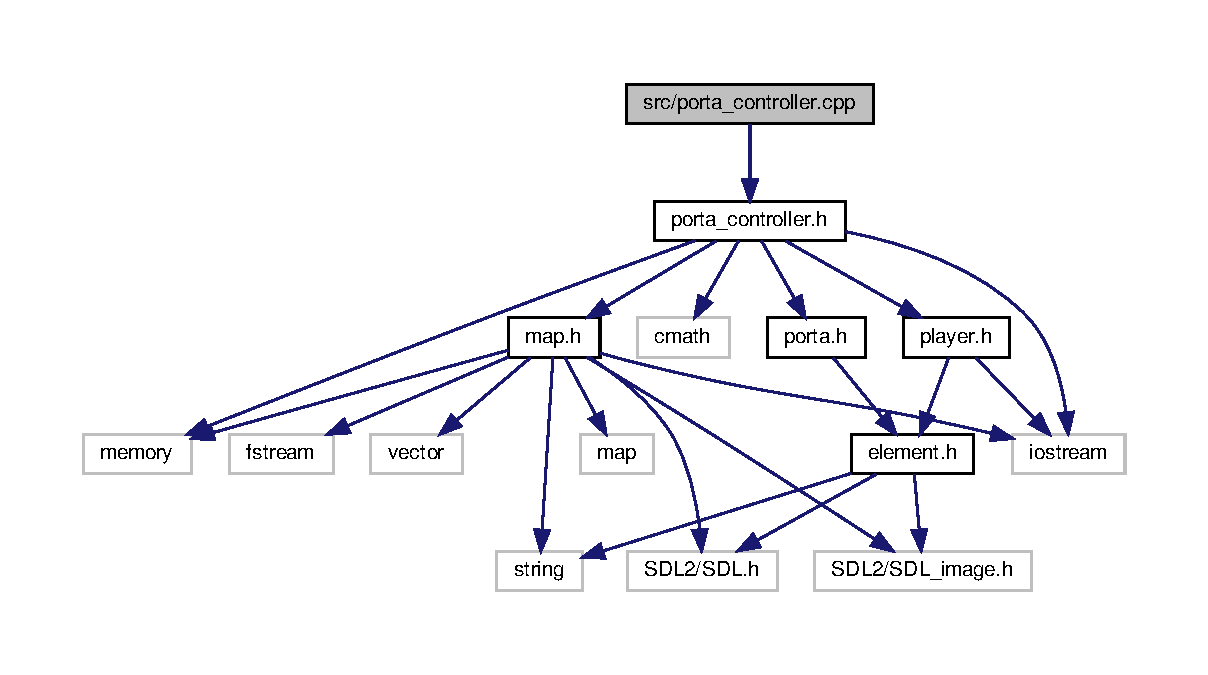
\includegraphics[width=350pt]{porta__controller_8cpp__incl}
\end{center}
\end{figure}

\hypertarget{viewer_8cpp}{}\section{src/viewer.cpp File Reference}
\label{viewer_8cpp}\index{src/viewer.\+cpp@{src/viewer.\+cpp}}
{\ttfamily \#include \char`\"{}viewer.\+h\char`\"{}}\newline
Include dependency graph for viewer.\+cpp\+:
\nopagebreak
\begin{figure}[H]
\begin{center}
\leavevmode
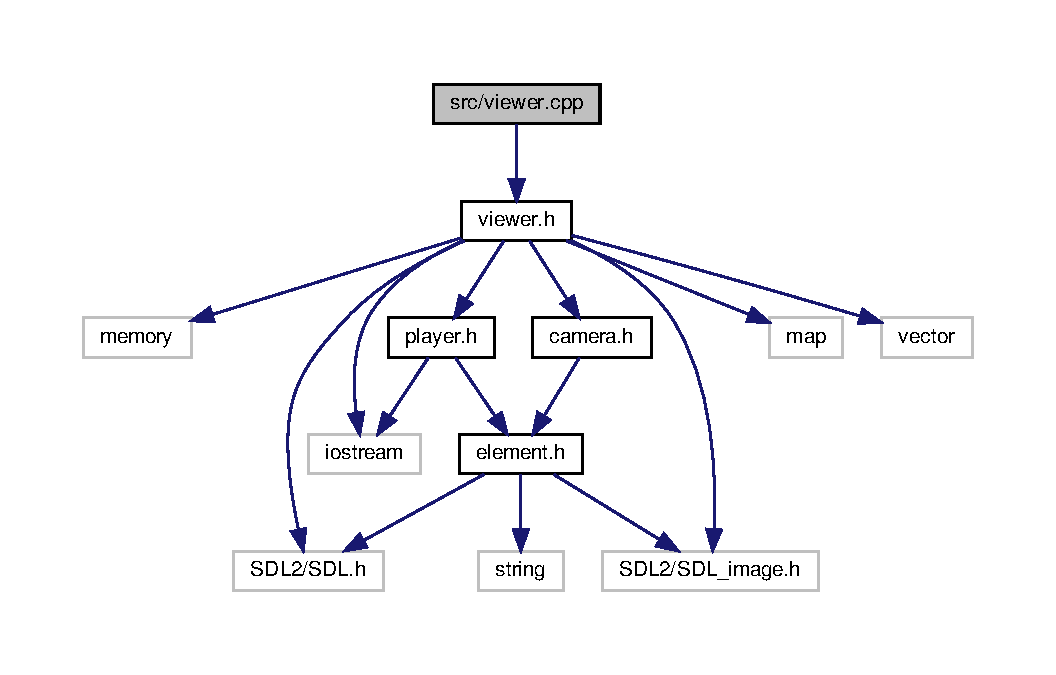
\includegraphics[width=350pt]{viewer_8cpp__incl}
\end{center}
\end{figure}

%--- End generated contents ---

% Index
\backmatter
\newpage
\phantomsection
\clearemptydoublepage
\addcontentsline{toc}{chapter}{Index}
\printindex

\end{document}
